% --------------------------------------------------------------------------
% Report template for BIR projects
% Report template with support for Portuguese and English languages
% Change language {brazil or english} in \documentclass as per the examples
% This template has support for the ABNT citing format
% 
% Original version: jan/2019
% https://github.com/
% 
% Based on ABNTEX2 and the thesis template
% --------------------------------------------------------------------------
\documentclass[
%\DeclareUnicodeCharacter{200B}{}
% --------------------------------------------------------------------------
% classe memoir . options                                                   
12pt,					% tamanho da fonte
openright,				% cap. começam em pág ímpar (ins pág vazia caso preciso)
twoside,				% para impressão em verso e anverso. Oposto a oneside
a4paper,				% tamanho do papel
% --------------------------------------------------------------------------
% classe abntex2 . options                                                  
%chapter=TITLE,			% títulos de capítulos convertidos em letras maiúsc.
%section=TITLE,			% títulos de seções convertidos em letras maiúsc.
%subsection=TITLE,		% títulos de subseções convertidos em letras maiúsc.
%subsubsection=TITLE,	% títulos de subsubseções convertidos em letras maiúsc.
% --------------------------------------------------------------------------
% Opções de IDIOMA do pacote babel                                          
english,
brazil
]{ABNT/abntex2_report}
% --------------------------------------------------------------------------
% Pacotes básicos    
\usepackage{lmodern}			% Usa a fonte Latin Modern			
\usepackage[T1]{fontenc}		% Selecao de codigos de fonte.
\usepackage[utf8]{inputenc}		% Codificacao do documento (conversão automática dos acentos)
\usepackage{indentfirst}		% Indenta o primeiro parágrafo de cada seção.
\usepackage{color}				% Controle das cores
\usepackage{graphicx}			% Inclusão de gráficos
\usepackage{microtype} 			% para melhorias de justificação
\usepackage{lipsum}	
\usepackage[brazilian,hyperpageref]{backref} % páginas com citações na bibliog.
%\usepackage[alf,abnt-etal-list=0,abnt-etal-cite=3,abnt-emphasize=bf]{abntex2cite}
\usepackage[alf]{abntex2cite}
%	
\usepackage{lastpage}			% Usado pela Ficha catalográfica
%\usepackage{subfig}
\usepackage{supertabular}       % tabela na capa do documento
\usepackage{booktabs}
\usepackage[table,xcdraw]{xcolor}
\usepackage{adjustbox}
\usepackage{amssymb,amsmath,mathrsfs}
\usepackage{algorithm,algpseudocode}
\usepackage{pgfplots}
\usepackage{tikz}
\usepackage{titlesec}
\usepackage{ragged2e}
\usepackage{tocloft}
\usepackage{threeparttable}
\usepackage{etoolbox}
\usepackage[normalem]{ulem}
\usepackage{yaacro}
\usepackage[none]{verlab}
%\usepackage{fontspec}
%\setmainfont{Helvetica Light}
\usepackage{lscape}
%\usepackage[graphicx]{realboxes}
\usepackage{rotating}
\usepackage{wrapfig}
\usepackage{caption}
\usepackage{subcaption}
\usepackage{dirtytalk}
\usepackage{pdfpages}
\usepackage{threeparttable}
\usepackage{hyperref}
%\hypersetup{draft}
\usepackage{float}
\usepackage{multirow}
\usepackage{enumitem}
\usepackage{listings}
\usepackage{listingsutf8}
%\usepackage[xindy={language=portuguese},subentrycounter,seeautonumberlist,nonumberlist=true]{glossaries}
%\usepackage[lofdepth,lotdepth]{subfig}
\DeclareUnicodeCharacter{200B}{}
% --------------------------------------------------------------------------%
% Configurações do PDF final                                                
\definecolor{blue}{RGB}{41,5,195}
\makeatletter
\hypersetup{
	%pagebackref=true,
	pdftitle={\@title}, 
	pdfauthor={\@author},
	pdfsubject={\@title},
	%pdfsubject={\imprimirpreambulo},
	pdfcreator={LaTeX with abnTeX2},
	pdfkeywords={abnt}{latex}{abntex}{abntex2}{\imprimirpalavraschave}, 
	colorlinks=true,       		% false: boxed links; true: colored links
	linkcolor=blue,          	% color of internal links
	citecolor=blue,        		% color of links to bibliography
	filecolor=magenta,      	% color of file links
	urlcolor=blue,
	bookmarksdepth=4
}
%\makeatother
% --------------------------------------------------------------------------
% Posiciona figuras e tabelas no topo da página quando adicionadas sozinhas
% em um página em branco. Ver https://github.com/abntex/abntex2/issues/170
%\makeatletter
\setlength{\@fptop}{5pt} % Set distance from top of page to first float
\makeatother
% --------------------------------------------------------------------------
% Formatação                                                                
\newcommand\tab[1][1cm]{\hspace*{#1}}
\apptocmd{\thebibliography}{\justifying}{}{} 
\renewcommand{\ABNTEXsectionfont}{\bfseries}
\titlespacing*{\chapter}{0pt}{0pt}{12pt}
\titlespacing*{\section}{0pt}{6pt}{6pt}
\titlespacing*{\subsection}{0pt}{6pt}{6pt}
\titlespacing*{\subsubsection}{0pt}{6pt}{6pt}
% --------------------------------------------------------------------------
% Rearranja os finais de cada estrutura                                     
\algrenewtext{EndWhile}{\algorithmicend\ \algorithmicwhile}
\algrenewtext{EndFor}{\algorithmicend\ \algorithmicfor}
\algrenewtext{EndIf}{\algorithmicend\ \algorithmicif}
\algrenewtext{EndFunction}{\algorithmicend\ \algorithmicfunction}
% --------------------------------------------------------------------------
% Espaçamentos entre linhas e parágrafos                                    
\setlength{\parindent}{1.3cm} % linha
\setlength{\parskip}{0.2cm} % parágrafo, tente também \onelineskip
% --------------------------------------------------------------------------
% Informações de dados para CAPA e FOLHA DE ROSTO                           
\prodtecnica{001 / 2020}
\titulo{Robô com Navegação Autônoma, detecção visual e manipulador}
% \tiporelatorio{} 
\nomeprojeto{Robô Autônomo}
\outrossubtitulos{~} % opcional
\autores{
	Anderson Queiroz do Vale \\
	Jéssica Lima Motta \\	
	Mateus Santos Cerqueira\
} 
\newcommand{\autoresexternos}{
	Lucas Cruz da Silva\\
	Rebeca Tourinho Lima\\
	Tiago Pereira de Souza\\
	Marco Antonio dos Reis\
}
\local{Salvador\\Bahia, Brasil}
\data{Novembro de 2020}
\classificacao{( ) Confidencial  (X) Restrito  ( )  Uso Interno  ( ) Público}
\revisao{01}
\tabelacutter{000} 
\palavraschave{1. Autonomous Navigation . 2. Manipulator. 3. Computer vision.}
\classificacaoassunto{000} % Número de Classificação do assunto 
%\parceirologo{logos/x.png}
%------------------------------------------------------------------
% Finalização das configurações da capa
%
%
%------------------------------------------------------------------              
% Acrônimos :: Chamar no texto como \ac{DoF}                                
\begin{acgroupdef}[list=acronyms]
	\acdef{AGV}{Automated Guided Vehicle}
	\acdef{CAD}{Computer Aided Design}
	\acdef{CCRoSA}{Centro de Competência de Robótica e Sistemas Autônomos}
	\acdef{DoF}{Degrees of Freedom}
	\acdef{FMECA}{Failure Modes, Effects and Critically Analysis}
	\acdef{OMPL}{Open Motion Planning Library}
	\acdef{OpenCV}{Open Source Computer Vision}
	\acdef{ROS}{Robot Operating System}
	\acdef{SOTA}{Study Of The Art}	
	\acdef{URDF}{Unified Robot Description Format}	
	
	
	%
	%
	%
\end{acgroupdef}
% --------------------------------------------------------------------------
% Criação do sumário
\makeindex
%
\begin{document}
	\frenchspacing
	\imprimircapa
	\imprimircatalografica
% --------------------------------------------------------------------------
% Sumário executivo                                                         
	\ABNTEXchapterfont\large\textbf{\execsummarytitlename}
	\begin{flushleft}
		\normalsize
		\justify
		\normalfont
		O projeto de Robô Autônomo- Desafio 3.0, também conhecido como \textbf{Saci} configura-se: sob o Programa de Formação de Novos Talentos do \ac{CCRoSA} do Serviço Nacional de Aprendizagem Industrial, Departamento Regional da Bahia - Senai/DR/BA, sendo este o principal fomentador do programa.  O presente trabalho tem como impulsionador principal a capacitação de novos pesquisadores preparados para solucionar os mais diversos problemas relacionados a robótica e sistemas autônomos.

		O projeto foi considerado como início técnico no dia 04 de Novembro de 2020.  
		
		O prazo de execução planejado foi de 30 dias.
	\end{flushleft}
	\clearpage
%------------------------------------------------------------------
% Resumo e abstract                                                         
	\ABNTEXchapterfont\large\textbf{\resumoatitlename}
	\begin{flushleft}
		\normalsize
		\justify
		\normalfont
		O Saci integra o robô da \textit{Clearpath Robotics Warthog} equipado com sensores (câmeras, LiDAR e GPS) e o manipulador robótico JeRoTIMON, com o propósito de transformá-lo em um robô autônomo. Este robô foi construído com o intuito de que o mesmo tivesse navegação autônoma para realizar investigação em ambiente externo e construir um mapa deste, detectasse a bomba escondida nesse ambiente, e realizasse o desarme da bomba através do manipulador. Para a simulação foram utilizados o software  \textit{Gazebo} e a ferramenta de visualização \textit{Rviz}, e para o manipulador foi utilizado \textit{MoveIt}. Este robô também possui sua versão real onde foi possível realizar testes e verificar seu desempenho em campo.		
	\end{flushleft}
	\vspace*{1cm}
	\newpage
	%
	\ABNTEXchapterfont\large\textbf{\resumobtitlename}
	\begin{flushleft}
		\normalsize
		\justify
		\normalfont
		PUT IN ENGLISH
	\end{flushleft}
	\clearpage
% --------------------------------------------------------------------------
% Lista de figuras                                                          
	\begin{flushleft}
		\ABNTEXchapterfont\Large\textbf{\MakeUppercase\listadefigurasname}
	\end{flushleft}
	\vspace*{-36pt}
	\pdfbookmark[0]{\listfigurename}{lof}
	\normalsize
	\listoffigures*
	\cleardoublepage
% --------------------------------------------------------------------------
% Lista de tabelas                                                          
	\begin{flushleft}
		\ABNTEXchapterfont\Large\textbf{\MakeUppercase\listadetabelasname}
	\end{flushleft}
	\vspace*{-36pt}
	\pdfbookmark[0]{\listtablename}{lot}
	\normalsize
	\listoftables*
	\cleardoublepage
% --------------------------------------------------------------------------
% Lista de símbolos e abreviaturas                                          
	\begin{flushleft}
	\ABNTEXchapterfont\Large\textbf{\MakeUppercase\listadesimbolsabrevtitlename}
		\noindent
		\vspace*{-06pt}
		\pdfbookmark[0]{\listadesiglasname}{lot}
		\normalsize
		\normalfont
		\aclist[list=acronyms]
	\end{flushleft}
	\newpage
% --------------------------------------------------------------------------
% Tabela de conteúdo                                                        	
	\begin{flushleft}
		\ABNTEXchapterfont\Large\textbf{\MakeUppercase\glosariotitlename}
	\end{flushleft}
	%\pagebreak
	\vspace*{-36pt}
	\pdfbookmark[0]{\contentsname}{toc}
	\normalsize
	\normalfont
	\tableofcontents*
	\justify
% --------------------------------------------------------------------------
% Formatação, remover espaço depois dos títulos
	\setlength\beforechapskip{-24pt}
	\setlength\afterchapskip{12pt}
	\textual
	\pagestyle{plain}
	\normalsize
	\justify
	\normalfont
% --------------------------------------------------------------------------
% Conteúdo do relatório  
	\chapter{INTRODUÇÃO}
\label{chap:intro}
A robótica é um campo relativamente jovem da tecnologia moderna que atravessa os limites da engenharia tradicional \cite{spong2005robot}. O estudo da robótica é um ramo da tecnologia que engloba área de mecânica, eletrônica e computação, com graus de teoria de controle, microeletrônica, inteligência artificial, fatores humanos e de produção \cite{pimenta}. Segundo \cite{erthal}, o crescimento da robótica na indústria é justificado em face das exigências de maior qualidade, produtividade e flexibilidade nos processos fabris. Na área industrial, a robótica evoluiu devido ao aumento de uso de robôs e manipuladores industriais.

O estudo do desenvolvimento de manipuladores robóticos foi iniciado por volta de 1954 com George Devol, quando foi desenvolvido o primeiro robô programável e desde então grandes desenvolvimentos nessa área foram atingidos. Como resultado desse avanço, o investimento de empresas foi em torno de 16,5 bilhões de dólares em 2018, chegando a marca de 420 mil unidades enviadas mundialmente, com perspectiva de crescimento médio de 12\% ao ano entre 2020 e 2022 \cite{ifr}.

Um manipulador robótico é um dispositivo mecânico composto de elementos rígidos (elos) que proporcionam a sustentação e alcance do braço. A inevitabilidade de apresentar algum grau de flexibilidade faz com que esses elos necessitem ser projetados para apresentar elevada rigidez aos esforços que o manipulador será submetido. Esses elos são conectados entre si através de articulações (juntas), que oferecem graus de liberdade ao manipulador e controle de movimento relativo entre os elos. Essas juntas podem ser basicamente divididas em dois grupos: juntas prismáticas e juntas de rotação. Neste projeto foram utilizadas juntas de rotação. A disposição dessas juntas determina a classificação dos manipuladores como Cartesianos, Esféricos, Cilíndricos, entre outros \cite{robindust}.

Este relatório descreve o processo de construção de um manipulador robótico desenvolvido no Centro de Competência em Robótica e Sistemas Autônomos do SENAI CIMATEC e é destinado ao programa de formação Novos Talentos. São descritas as etapas de concepção, simulação, testes e implementação física.


%------------------------------------------------------------------
\section{Objetivos}
\label{sec:obj}
O propósito deste projeto é construir um manipulador robótico capaz de identificar um marcador visual por meio de uma câmera RGB e proceder com a função de acionar um painel elétrico. 
Para isso, os objetivos específicos são:
\begin{itemize}
  \item  Realizar estudo do Estado da Arte(\textit{\acs{SOTA}}) sobre manipuladores.
  \item  Realizar testes e parametrização dos servomotores.
  \item  Propor um modelo de manipulador robótico.
  \item  Parametrizar o pacote de reconhecimento de marcadores visuais. 
  \item  Desenvolver um pacote de configuração do \textit{MoveIt}.
  \item  Desenvolver o código para realizar a missão. 
  \item  Realizar a simulação do protótipo do manipulador em software.   
  \item  Implementar a versão física do protótipo.
  \item  Realizar testes e estudos estatísticos.
\end{itemize} 
%------------------------------------------------------------------
\section{Justificativa} %motivação
\label{sec:just}

  Apesar da crescente demanda, há falta de profissionais habilitados à desenvolver pesquisas e aplicações na área da robótica. O presente trabalho tem como impulsionador principal a capacitação de novos pesquisadores preparados para solucionar os mais diversos problemas relacionados a robótica e sistemas autônomos.

  A busca por melhor eficiência e precisão na realização de atividades em locais que a presença do ser humano torna-se difícil, arriscado e até mesmo impossível, vem se tornando cada vez maior no cotidiano dos ambiente industriais. Além disso, é importante a capacidade do robô de interagir com o ambiente a partir da captura e análise de estímulos visuais \cite{leite2005controle}. 

  Este projeto traz, dentre os benefícios, a utilização  de manipuladores robóticos autônomos que sejam capazes de identificar marcadores visuais e realizar tarefas que possam ser perigosas e/ou repetitivas para o ser humano. Espera-se que este projeto seja continuado e que seus resultados sejam compartilhados na comunidade científica, contribuindo para a construção de outros manipuladores com características e/ou objetivos semelhantes.
  



%------------------------------------------------------------------
\section{Organização do relatório}
\label{sec:org}
O presente relatório está organizado em oito capítulos, sendo este de introdução e descrição da justificativa/motivação dos objetivos e da organização do documento.

No capítulo \ref{chap:conce}, Conceito do Sistema, são descritos  parâmetros básicos do projeto, dentre eles os requisitos do cliente, requisitos técnicos e o estudo do estado da arte.

O capítulo \ref{chap:desenv}, Desenvolvimento do Sistema, apresenta a descrição do sistema onde serão apresentados a arquitetura geral, especificações técnicas, o ambiente de operação do manipulador e a estrutura analítica do protótipo. Além disso, trará as especificações funcionais que compõem o sistema, sua arquitetura de software e o que foi desenvolvido para simulação. 

O capítulo \ref{chap:implementacao}, Implementação, explica a construção física do manipulador. São expostos seus parâmetros de configuração e sua estrutura. 

O capítulo \ref{chap:result}, Resultados e Análises, são apresentados os resultados alcançados e a análise dos dados amostrados através de estudos estatísticos. 

O capítulo \ref{chap:conf}, Confiabilidade do Sistema, detalha a análise dos modos e efeitos de falhas.

No capítulo \ref{chap:conhec}, Gestão do Conhecimento, é feito um estudo sobre as lições aprendidas além de apresentar o guia de uso.

Por fim, o capítulo \ref{chap:conclu} apresenta a conclusão do relatório.



	\chapter{CONCEITO DO SISTEMA}
\label{chap:conce}
A norma técnica (ISO-8373, 2012) criada para padronizar o vocabulário referente aos
robôs e dispositivos robóticos operando em ambientes industriais e não industriais, define o manipulador como uma máquina na qual o mecanismo, geralmente, consiste em uma série de segmentos, articulados ou deslizantes entre si, com o objetivo de empunhar e/ou mover objetos (peças ou ferramentas) em vários graus de liberdade. Em outras palavras, um manipulador é um equipamento programável baseado em atuadores, com um certo grau de liberdade, projetado para realizar uma variedade de atividades, assim como realização de diversos processos industriais \cite{ISO8373}.

Neste capítulo serão tratados os requisitos solicitados pelo cliente, os requisitos técnicos do projeto, o estudo do estado da arte sobre manipuladores e o ambiente de operação em que este manipulador realizará a atividade.

%------------------------------------------------------------------
\section{Parâmetros básicos}
\label{sec:basi}
Nesta seção encontram-se os requisitos solicitados pelo cliente, ou seja, a tarefa que precisa ser realizada e em qual ambiente o manipulador será simulado e concebido. Além disso, são exibidos os requisitos técnicos que tratam das especificações do sistema e uma breve revisão teórica de conceitos relacionados ao manipulador.

\subsection{Requisitos do cliente}
\label{sub:reqc}
Requisitos predeterminados pelo cliente consistem em exigências de funcionamento que devem ser observadas ao final do projeto, para que se considere um sucesso a concepção deste. Para tal, foram determinadas algumas característica desejáveis no projeto:
\begin{enumerate}
    \item Desenvolver um manipulador robótico.
    \item Realizar a tarefa de detecção de um marcador visual e acionamento do painel elétrico na orientação vertical e horizontal.
    \item Realizar a simulação do manipulador no ambiente \textit{\acs{ROS}} utilizando o software \textit{Gazebo}.
    \item Utilizar o \textit{framework} \textit{MoveIt} para o controle do  manipulador. 
    \item Realizar estudo estatístico para verificação da performance do manipulador.    
\end{enumerate}

\subsection{Requisitos técnicos}
\label{sub:reqt}
Os requisitos técnicos de um projeto são especificações necessárias para o funcionamento esperado do projeto. Podem ser sobrepostos aos requisitos do cliente em caso de conflito entre o esperado pelo cliente e o necessário para que o projeto seja bem sucedido, objetivando manter o projeto o mais eficiente dentro do escopo planejado. Os requisitos foram:
\begin{enumerate}
    \item O manipulador deve estar acoplado em uma base fixa situada a 0,28 m de uma das extremidades da bancada e centralizada com a mesma.
    \item Utilizar servo motores Dynamixel PH54-200-S500-R, PH54-100-S500-R e PH42-020-S300-R da Robotis. 
    \item Conter uma câmera RGB Teledyne Dalsa Genie Nano C2590. 
    \item Deverá possuir 5 graus de liberdade.
    \item Suportar uma carga máxima de 2 kg. 
    \item Ser capaz de acionar um painel elétrico.
    %\item Detecção de uma  \textit{tag} fixada a um painel elétrico. 
\end{enumerate}

\subsection{Estudo do estado da arte}
\label{sub:sota}

\par Com o advento do exponencial crescimento da tecnologia há um foco crescente na pesquisa e comercialização de robôs \cite{hernandez2018education}. Estes, por sua vez, são classificados em três grupos: manipuladores, veículos auto-guiados (\textit{\acs{AGV}}) e robôs móveis. Neste projeto, o objeto de interesse são os manipuladores robóticos, sistemas que possuem estrutura física similar a um braço humano. Estes robôs são compostos por partes rígidas, denominado de elos, conectados entre si por juntas \cite{santos2004robotica}. Esta estrutura encontra-se descrita na Figura \ref{fig:manipulador}.

\begin{figure}
    \caption{Elos e junta de um manipulador robótico.}
    \centering
    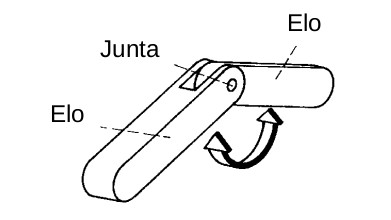
\includegraphics[scale=0.6]{images/manipulador.jpg}
    \legend{Fonte: \cite{santos2004robotica}.}
    \label{fig:manipulador}
\end{figure}

\par Muitas pesquisas vêm sido realizadas na área de manipuladores robóticos. Em \cite{hernandez2017design} é descrito o desenvolvimento de um manipulador robótico com 3 \textit{\acs{DoF}} e dois dedos independentes. Este robô foi desenvolvido com o propósito de manipular objetos, cujas localizações são conhecidas, e transportá-los de uma localidade para outra utilizando \textit{\acs{ROS}}. Os autores utilizaram o \textit{MoveIt} para tratar do planejamento de trajetória e o \textit{Rviz} como ferramenta de visualização. Além disso, foi desenvolvido um controlador de posição e força para o \textit{endeffector}\footnote{Na robótica, um endeffector é o dispositivo no final de um braço robótico, projetado para interagir com o meio ambiente.} durante o processo de \textit{pick and place}\footnote{Sequência de movimentos na qual o manipulador robótico pega determinado objeto e o transfere a uma pose alvo.}. Os experimentos realizados trouxeram bons resultados para o que foi proposto, sendo ressaltada a necessidade de adicionar um sistema de visão que permita identificar e localizar o objeto alvo. 

O planejamento de trajetória para um manipulador de 5 \textit{\acs{DoF}} a partir do \textit{MoveIt} é exibido em \cite{zhang2019motion}. A partir de um  modelo \textit{\acs{CAD}} já existente foi construído o modelo \textit{\acs{URDF}} utilizado para simulação no \textit{\acs{ROS}}. O processo de planejamento foi visualizado a partir do \textit{Rviz} e o caminho planejado foi transmitido para os servo-motores possibilitando ao manipulador executar a sua rotina. O robô tem como tarefa manipular um objeto alvo de um local para outro, identificado a partir de técnicas de visão computacional que combinam os algoritmos \textit{SIFT} e \textit{RANSAC}. OS resultados experimentais mostraram que o uso do \textit{MoveIt} reduz as dificuldades de operação para manipuladores e oferece vantagens em termos de validação de algoritmos e exploração de funções, sendo possível utilizar o método proposto para o controle em tempo real do robô. 

\par A aplicação de técnicas de visão computacional em um manipulador do tipo \textit{Robai Cyton Gamma 3000} é exibida em \cite{khan2018ros}. O robô é conectado com uma câmera externa via \textit{\acs{ROS}}, possui um \textit{endeffector} em forma de garra que segura uma estrutura similar a um prato, e tem como tarefa equilibrar uma bola localizada no centro do prato. Para realizar o controle da tarefa de equilíbrio, a bola é identificada a partir de um algoritmo escrito em C++ e que utiliza bibliotecas do \textit{\acs{OpenCV}}. As juntas do manipulador são atuadas a partir de servo-motores \textit{Dynamixel} que são diretamente controlados por um algoritmo. O sistema foi desenvolvido de forma que os componentes se comunicassem entre si para receber respostas do sistema de visão e dos motores, computá-las e enviar comandos de controle que permitissem executar a tarefa. Foram realizados testes e os resultados experimentais foram satisfatórios, sendo o manipulador capaz de equilibrar a bola em uma pequena vizinhança do centro do prato.

O uso de marcadores visuais do tipo \textit{ArUco} associados ao planejamento de trajetória para um manipulador robótico é abordado em \cite{javeed2019autonomous}. O manipulador encontra-se acoplado a uma plataforma móvel e tem como objetivo o transporte de objetos de forma autônoma em um determinado espaço. Os autores também descrevem a integração dos mecanismos de detecção do marcador visual, navegação do robô e planejamento de trajetória, realizados no \textit{\acs{ROS}}. O robô é capaz de estimar a pose do marcador, aproximar-se e realizar sua tarefa. Os testes realizandos mostraram a eficiência do sistema, sendo apontada a necessidade de um estudo futuro para possibilitar o planejamento de trajetória em um ambiente com obstáculos.
% \par Para que um manipulador possa se movimentar em um ambiente e realizar as tarefas propostas é necessário que sejam conhecidos sua orientação e posição em relação ao sistema de origem. Este conjunto de informações é denomidado de frame do robô e esta descrição constitui o sistema de referência de um manipulador robótico. Há sistemas transladados: onde a origem de um sistema está transladada em relação ao do manipulador; sistemas rotacionados: as origens do sistema de referência coincidem, porém um dos sistemas tem um dos eixos rotacionados em um ângulo $\alpha$ em relação ao outro; e há o sistema genérico, neste sabe-se a descrição de um vetor em relação a um sistema de referência. 

% Uma das primeiras 
% Para realizar o mapeamento genérico, cinemática direta, utiliza-se a Equação \ref{map_generico} onde $_{ }^{A}\textrm{P}$ é o vetor de posição no sistema de referência {A} descrevendo os pontos x, y e z deste sistema. Através da matriz de transformação homogênea, ${_{B}^{A}\textrm{T}}$ é possível realizar o mapeamento do manipulador em um sistema de referência em relação a outro, neste caso de {B} em relação a {A}. Esta matriz de transformação homogênea engloba as matrizes de rotação do sistema B em relação a A, ${_{B}^{A}\textrm{R}}$, e do vetor posição que localiza a origem do sistema de B $_{ }^{A}\textrm{P}_{BORG}$ \cite{mckerrow1991introduction}. 

% \begin{equation}
%     \label{map_generico}
%     _{ }^{A}\textrm{P} = {_{B}^{A}\textrm{T}} {_{ }^{B}\textrm{P}}    
% \end{equation}


% \par O estudo da dinâmica e da cinemática apresenta a síntese do projeto de um dispositivo, expressando matematicamente as relações de movimento de um mecanismo na execução de determinada tarefa.

% \par Após as configurações do sistema é necessário encontrar as equações de dinâmicas de movimento que podem ser obtidas pelo método de equações de movimento de Newton ou utilizando o cálculo variacional (Princípio de Hamilton ou Princípio da Mínima Ação) \cite{lima2017dinamica}.

% \par Para a análise cinemática, utiliza-se os parâmetros de Denavitt-Hartenberg (D-H). Este realiza uma cadeia cinemática espacial através da fixação de sistemas de referência aos elos \cite{paul1981robot}.  Esta notação de Denavit-Hartenberg é uma ferramenta comumente utilizada para sistematizar a descrição cinemática de sistemas mecânicos articulados com $\textit{n}$
% graus de liberdade \cite{uicker1964iterative}. Na Tabela \ref{tab:dh_table} tem-se a cadeia cinemática através dos parâmetros D-H para o manipulador da Figura \ref{fig:cinematica}, nesta tabela tem-se o elo (\textit{link}), $\theta$ refere-se ao ângulo de rotação no eixo z e $\alpha$ rotação no eixo x, \textit{a} refere-se a translação ao longo do eixo de rotação x e \textit{d} translação ao longo do eixo z. Na cinemática direta é possível observar que a partir dos ângulos das juntas do manipulador encontra-se a posição e orientação da ferramenta com relação a estação de trabalho. Contudo, quando projeta-se um manipulador, é fundamental realizar os cálculos da cinemática inversa. Nesta, por sua vez, são obtidos dados de posição e orientação da ferramenta com relação a estação de trabalho e calcula-se os ângulos das juntas \cite{craig2012robotica}.

% \par Para encontrar os ângulos de juntas necessários para posiocionar o sistema de referência da ferramenta (\textit{tool frame}) com relação ao sistema da estação de trabalho (\textit{station frame}), divide-se em duas partes. Primeiro, fazemos as transformações para encontrar o sistema do punho (\textit{wrist frame}) com relação ao sistema da base (\textit{base frame}) e depois usa-se a cinemática inversa para calcular os ângulos das juntas. O cálculo desses ângulos possibilita a construção de sistemas de controle que tradicionalmente utilizam matrizes jacobianas em conjunto com as pseudo-inversas \cite{wunderlich2004simulating}.

% \par  As soluções mais utilizadas para calcular a cinemática inversa são os métodos analíticos e numéricos iterativos. A escolha de um método depende de sua aplicação, do tipo de junta, da estrutura utilizada e da quantidade de graus de liberdade. Na maioria dos casos o método numérico é preferível quando se tem acesso ao um processamento computacional adequado. Existem diversos métodos numéricos iterativos, exemplo: O Newton-Raphson, algoritmo de Levenberg–Marquardt, o Jacobiano Pseudo-Inverso \cite{pinheiro2013cinematica}.




% \begin{figure}
%     \caption{Frames para o manipulador Elbow.}
%     \centering
%     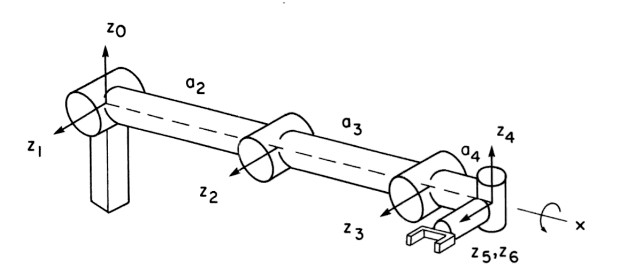
\includegraphics[scale=0.6]{images/cinematica.jpg}
%     \legend{Fonte: \cite{paul1981robot}.}    
%     \label{fig:cinematica}
% \end{figure}


% \begin{table}[H]
%     \caption{Parâmetros dos links para o manipulador Elbow.}
%     \centering
%     \begin{tabular}{|c|c|c|c|c|c|c|}
%     \hline
%     \textbf{Link} & \textbf{Variável}     & \textbf{$\alpha$} & \textbf{a} & \textbf{d} & \textbf{$\cos{\alpha}$} & \textbf{$\sin{\alpha}$} \\ \hline
%         1             & $\theta_{1}$ & 90º                            & 0          & 0          & 0                                  & 1                                   \\ \hline
%         2             & $\theta_{2}$                      & 0º                             & $a_{2}$         & 0          & 1                                  & 0                                   \\ \hline
%         3             & $\theta_{3}$                      & 0º                             & $a_{3}$         & 0          & 1                                  & 0                                   \\ \hline
%         4             & $\theta_{4}$                      & -90º                           & $a_{4}$         & 0          & 0                                  & -1                                  \\ \hline
%         5             & $\theta_{5}$                      & 90º                            & 0          & 0          & 0                                  & 1                                   \\ \hline
%         6             & $\theta_{6}$                      & 0º                             & 0          & 0          & 1                                  & 0                                   \\ \hline
%     \end{tabular}
%     \legend{Fonte: \cite{paul1981robot}.}
%     \label{tab:dh_table}
% \end{table}


% O controle da cinemática e o planejamento da movimentação evitam que o manipulador colida com outros elementos do seu espaço de trabalho. Para tal é necessário aplicar técnicas de controle e utilização de sensores, estes últimos fazem com que o robô tenha capacidade de percepção coletando dados tanto internos, sobre seu sistema mecânico, quanto externos, no meio ambiente em qual está inserido \cite{sciavicco2012modelling}.

% A dinâmica do manipulador dependerá do seu design mecânico, logo esta definição irá variar de um manipulador para outro, e depende também de já haver definido as formulações cinemáticas \cite{norton2001mecanismos}. Estas por sua vez, fornecem os elementos geométricos de um sistema que são a base para se obter as energias que compõem as equações dinâmicas.

% 
% \subsection{Características do manipulador}
% \label{sub:carac}
% Na Tabela \ref{tab:dh} encontra-se os parâmetros relacionados aos elos do manipulador Timon-HM descrito conforme a Figura \ref{fig:dh_config}.
% //todo uma subsection só para apresentar uma tabela?? porque? não faz sentido

% \begin{figure}[H]
%     \caption{Configuração D-H do manipulador Timon-HM.}
%     \centering
%     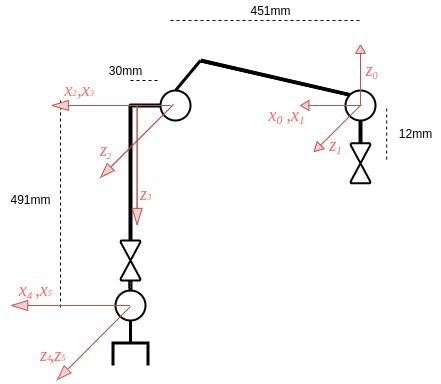
\includegraphics[scale=0.8]{images/dh_configuration.png}
%     \legend{Fonte: Autoria própria.}
%     \label{fig:dh_config}
% \end{figure}

% \begin{table}[H]
%     \caption{Parâmetros D-H para o manipulador Timon-HM.}
%     \centering
%     \begin{adjustbox}{max width=\textwidth}
%     \begin{tabular}{|c|c|c|c|c|}
%     \hline
%     \rowcolor[HTML]{EFEFEF} 
%     Link & a (mm) & $\alpha $(rad) & d (mm) & $\theta $(rad) \\ \hline
%     1 & 0   & $\pi / 2$ & 12  & 0                     \\ \hline
%     \rowcolor[HTML]{EFEFEF} 
%     2 & 452 & 0         & 0   & $\pi/2 - \arctan(30/451)$ \\ \hline
%     3 & 30  & $-\pi/2$  & 0   & $\pi/4 + \arctan(30/451)$ \\ \hline
%     \rowcolor[HTML]{EFEFEF} 
%     4 & 0   & $\pi/2$   & 491 & 0                     \\ \hline
%     5 & 0   & 0         & 0   & 0                     \\ \hline
%     \end{tabular}
%     \end{adjustbox}
%     \legend{Fonte: Autoria própria.}
%     \label{tab:dh}
%     \end{table}



% \subsection{Ambiente de operação}
% \label{sub:ambiente}
% //TODO lembrem-se não é caixa, é um painel elétrico:
% //TODO Jess corrigido
% O ambiente para a realização do desafio, onde serão incluídos o manipulador e um painel elétrico, é sobre uma mesa com 1.7 m de comprimento por 0.8 m de largura. Na Figura \ref{fig:simulacao} tem-se o ambiente de operação simulado no Gazebo para que possam ser realizados testes e para validação dos parâmetros aplicados ao manipulador.

% \par Nas Figuras \ref{fig:workspace_xy}, \ref{fig:workspace_xz} e \ref{fig:workspace_yz} estão descritos o \textit{workspace}, ambiente de operação do manipulador com as vistas dos eixos X-Y, X-Z e Y-Z, respectivamente. 
% A região em azul indica onde o manipulador consegue operar e a partir destas imagens é possível observar que o manipulador possui restrições de operação. Isso é devido às limitações existentes em cada junta.

% \begin{figure}[H]
%     \caption{Simulação no Gazebo}
%     \centering
%     \includegraphics[scale=0.34]{images/desafio.png}
%     \legend{Fonte: Autoria própria.}
%     \label{fig:simulacao}
% \end{figure}


% \begin{figure}[H]
%     \caption{Workspace do manipulador nos eixos X-Y.}
%     \centering
%     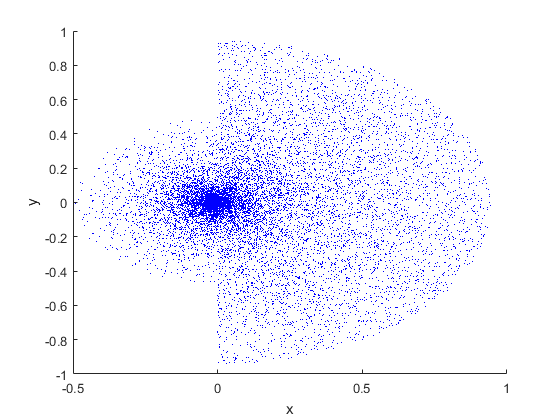
\includegraphics[scale=0.8]{images/workspace_xy.png}
%     \legend{Fonte: Autoria própria.}
%     \label{fig:workspace_xy}
% \end{figure}



% \begin{figure}[H]
%     \caption{Workspace do manipulador nos eixos X-Z.}
%     \centering
%     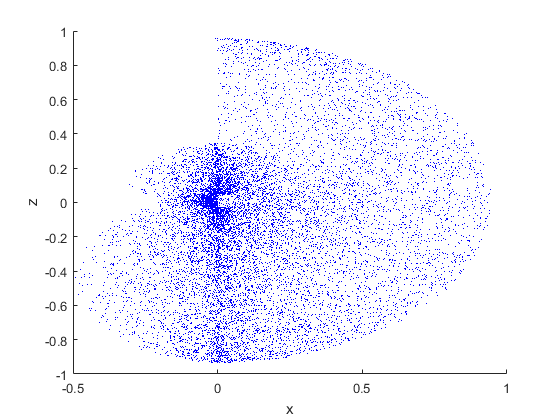
\includegraphics[scale=0.8]{images/workspace_xz.png}
%     \legend{Fonte: Autoria própria.}
%     \label{fig:workspace_xz}
% \end{figure}


% \begin{figure}[H]
%     \caption{Workspace do manipulador nos eixos Y-Z.}
%     \centering
%     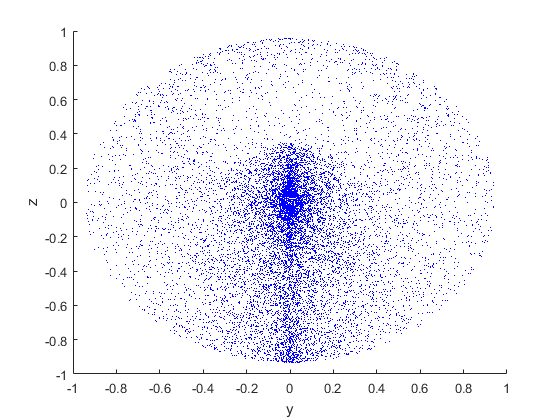
\includegraphics[scale=0.8]{images/workspace_yz.png}
%     \legend{Fonte: Autoria própria.}
%     \label{fig:workspace_yz}
% \end{figure}


%\subsection{Normas utilizadas}
%\label{sub:normas}

%EXTRA
%\subsection{Benchmarking}
%\label{sub:bench}

%EXTRA
%\subsection{Desdobramento da Função Qualidade}
%\label{sub:qfd}

%EXTRA
%\subsection{Matriz morfológica}
%\label{sub:matmorf}



	\chapter{DESENVOLVIMENTO DO SISTEMA}
\label{chap:desenv}
Nesta seção serão explicitadas as características do manipulador JeRoTIMON, abordando os sistemas que o compõem em \textit{software} e em \textit{hardware}. Suas funcionalidades principais são abordadas e a conexão entre as mesmas é exibida. 

%------------------------------------------------------------------
\section{Descrição do sistema}
\label{sec:descsis}

JeRoTIMON é um manipulador desenvolvido para atender às demandas relacionadas ao reconhecimento de marcadores visuais e, a partir desta identificação, realizar o acionamento de um painel elétrico. Os pacotes que constituem este robô foram concebidos através do \textit{software} de simulação \textit{Gazebo}, da ferramenta de visualização \textit{Rviz} e do \textit{framework}\footnote{São conjuntos de aplicações dentro de um projeto que interagem entre si e com isso se alcança resultados como uma determinada função de um programa.} para planejamento de trajetória \textit{MoveIt}. O uso dessas ferramentas possibilita que uma grande variedade de atividades que venham a ser realizadas no mundo real tenham sido previamente testadas em ambiente computacional.

\subsection{Arquitetura geral}
\label{sub:arqg}

A Figura \ref{fig:arquitetura_geral} ilustra a estruturação do sistema e a relação entre \textit{software} e \textit{hardware}. As cores representam o sistema geral(salmão), sistema operacional(verde), \textit{framework}(roxo) e pacotes(azul).
\begin{figure}[H]
  \caption{Arquitetura geral do sistema.}
  \centering
  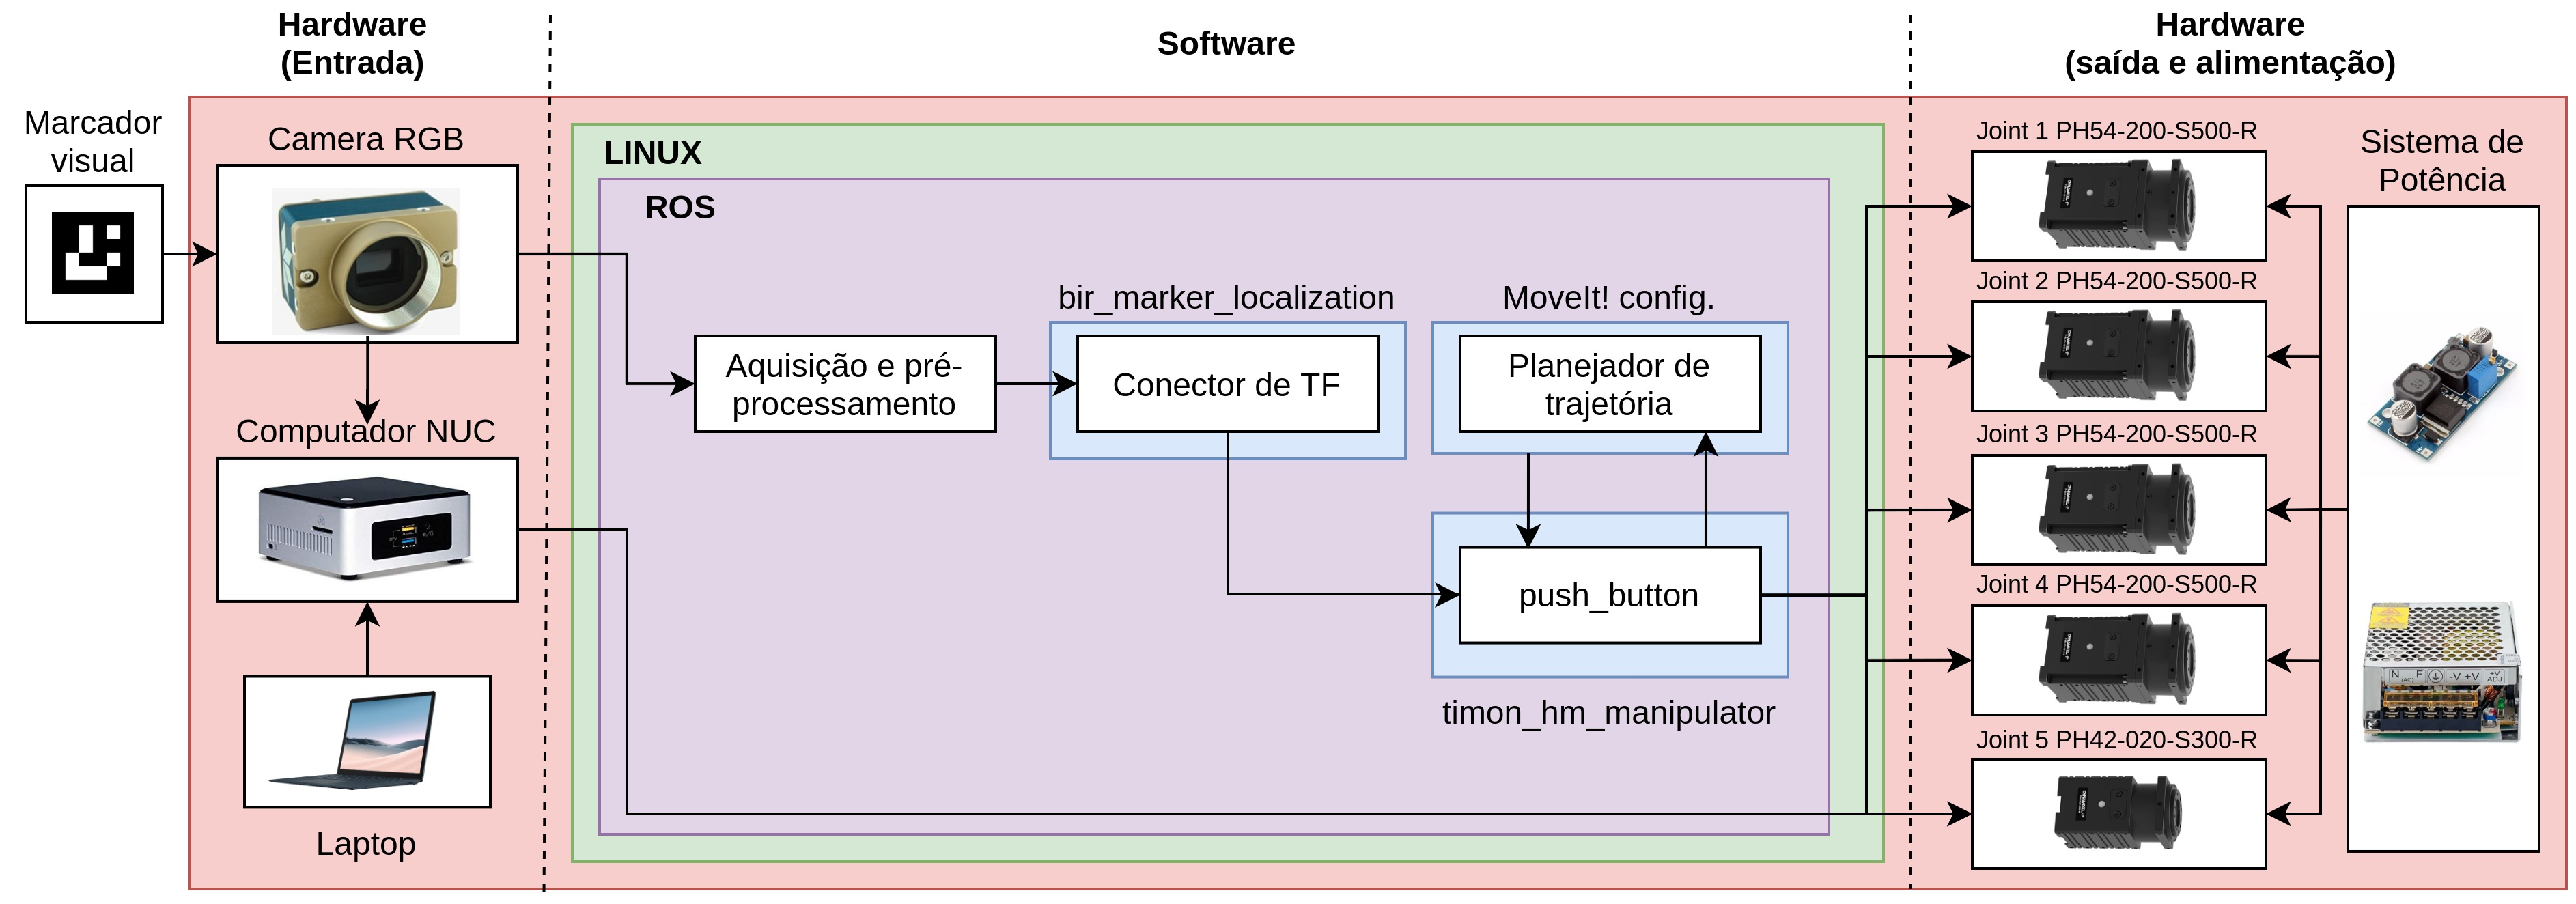
\includegraphics[width=16 cm]{images/arquitetura_geral.jpg}
    \label{fig:arquitetura_geral}
  \legend{Fonte: Autoria própria.}
\end{figure}

Um laptop, conectado via acesso remoto, dá início a aplicação no computador \textit{NUC}\footnote{Computador pequeno, completo e altamente eficiente energeticamente.} que possui instalado o software do protótipo.  Com o sistema iniciado, a câmera RGB é capaz de obter dados visuais do ambiente e enviá-los para o \textit{\acs{ROS}}.  Ao encontrar o marcador visual, o pacote \textit{bir\_marker\_localization} é capaz de unir as árvores de \textit{TF}\footnote{Pacote do \textit{\acs{ROS}} que permite verificar as relações entre os \textit{frames} na estrutura de árvore.} do painel elétrico e do manipulador, que antes encontravam-se desconectadas. Esta conexão, garante que sejam conhecidos os dados de posição ao nó \textit{push\_button} possibilitando o planejamento de trajetória para o ponto desejado. Com o caminho planejado, \textit{push\_button} pode enviar os comandos para cada junta do manipulador, onde encontram-se os motores \textit{Dynamixel} que são alimentadas pelo sistema de potência.

\subsection{Especificação técnica}
\label{sub:esptec}

Na Tabela \ref{tab:esp_table} estão elencadas as especificações técnicas do manipulador robótico JeRoTIMON. O numero de Graus de Liberdade foi definido baseado na capacidade de movimentação necessária para a realização dos desafios propostos. A carga útil, peso e o alcance máximo foram calculados com o auxilio do \textit{software} \textit{Onshape}, uma alternativa ao cálculo manual. A faixa de operação dos motores foi obtida segundo os limites de segurança observados, o que acrescenta proteção principalmente ao cabeamento do sistema. Informações a respeito de componentes como câmeras e motores seguem o seu padrão original de fabricação.

% \begin{table}[H]
%   \caption{Especificações técnicas do manipulador JeRoTIMON.}
%   \centering
%   \begin{tabular}{|c|c|}
%   \hline
%   \textbf{Item}                                                  & \textbf{JeRoTIMON}                                               \\ \hline
%   Graus de liberdade                                             & 5                                                               \\ \hline
%   \rowcolor[HTML]{EFEFEF} 
%   Carga útil                                                     & 1,94 kg                                                         \\ \hline
%   Alcance                                                        & \cellcolor[HTML]{FFFFFF}979 mm                                  \\ \hline
%   \rowcolor[HTML]{EFEFEF} 
%   Peso                                                           & 7,38 kg                                                         \\ \hline
%   Tensão de operação                                             & 24 V                                                            \\ \hline
%   \rowcolor[HTML]{EFEFEF} 
%   \cellcolor[HTML]{EFEFEF}                                       & Junta 1, Junta 2: 1.003.846 pulsos/rev                          \\ \cline{2-2}
%   \multirow{-2}{*}{\cellcolor[HTML]{EFEFEF}Resolução}            & Junta 3, Junta 4, Junta 5: 4096 pulsos/rev                       \\ \hline
%                                                                  & \cellcolor[HTML]{EFEFEF}Junta 1, Junta 2: H54-200-S500-R (200 W) \\ \cline{2-2}
%   \multirow{-2}{*}{Motores}                                      & Junta 3(2), Junta 4, Junta 5: MX-106 (65 W)                      \\ \hline
%   \rowcolor[HTML]{EFEFEF} 
%   \cellcolor[HTML]{EFEFEF}                                       & Junta 1: $ -90^\circ \sim 90^\circ $                      \\ \cline{2-2} 
%   \cellcolor[HTML]{EFEFEF}                                       & Junta 2: $ -90^\circ \sim 90^\circ $                      \\ \cline{2-2} 
%   \rowcolor[HTML]{EFEFEF} 
%   \cellcolor[HTML]{EFEFEF}                                       & Junta 3: $ -90^\circ \sim 135^\circ $                     \\ \cline{2-2} 
%   \cellcolor[HTML]{EFEFEF}                                       & Junta 4: $ -180^\circ \sim 180^\circ $                           \\ \cline{2-2} 
%   \rowcolor[HTML]{EFEFEF} 
%   \multirow{-5}{*}{\cellcolor[HTML]{EFEFEF}Faixa de operação}    & Junta 5: $ -90^\circ \sim 90^\circ $                      \\ \hline
%   Camera                                                         & Teledyne Genie Nano C2590                                             \\ \hline
%   \rowcolor[HTML]{EFEFEF} 
%   \cellcolor[HTML]{EFEFEF}                                       & Pose inicial: Codificador Absoluto                                        \\ \cline{2-2} 
%   \multirow{-2}{*}{\cellcolor[HTML]{EFEFEF}Tipo do sensor de posição} & Controle: Codificador Incremental                                    \\ \hline
%   Communicação                                                   & RS485                                                           \\ \hline
%   \rowcolor[HTML]{EFEFEF} 
%   Taxa de transmissão                                            & 1 Mbps                                                          \\ \hline
%   \end{tabular}
%   \legend{Fonte: Autoria própria.}
%   \label{tab:esp_table}
%   \end{table}



  \begin{table}[H]
    \caption{Especificações técnicas do manipulador JeRoTIMON.}
    \begin{tabular}{|c|c|}
    \hline
    \rowcolor[HTML]{EFEFEF} 
    \textbf{Item}                                              & \textbf{JeRoTIMON}                                             \\ \hline
    \textbf{Graus de liberdade}                                & 5                                                              \\ \hline
    \rowcolor[HTML]{EFEFEF} 
    \textbf{Carga útil}                                        & 2 {[}kg{]}                                                     \\ \hline
    \textbf{Alcance}                                           & 981 {[}mm{]}                                                   \\ \hline
    \rowcolor[HTML]{EFEFEF} 
    \textbf{Peso (sem base)}                                   & 6,4 {[}kg{]}                                                   \\ \hline
    \textbf{Peso (com base)}                                   & 10 {[}kg{]}                                                    \\ \hline
    \rowcolor[HTML]{EFEFEF} 
    \textbf{Tensão de operação}                                & 24 {[}V{]}                                                     \\ \hline
                                                               & Junta 1, Junta 2, Junta 3, Junta 4: 1,003,846 {[}pulsos/rev{]} \\ \cline{2-2} 
    \multirow{-2}{*}{\textbf{Resolução}}                       & Junta 5: 607,500 {[}pulsos/rev{]}                              \\ \hline
    \rowcolor[HTML]{EFEFEF} 
    \cellcolor[HTML]{EFEFEF}                                   & Junta 1, Junta 2, Junta 3: PH54-200-S500-R (200 W)             \\ \cline{2-2} 
    \rowcolor[HTML]{EFEFEF} 
    \cellcolor[HTML]{EFEFEF}                                   & Junta 4: PH54-100-S500-R (100W)                                \\ \cline{2-2} 
    \rowcolor[HTML]{EFEFEF} 
    \multirow{-3}{*}{\cellcolor[HTML]{EFEFEF}\textbf{Motores}} & Junta 5: PH42-020-S300-R (20 W)                                \\ \hline
                                                               & Junta 1: $ -45^\circ \sim 45^\circ $                           \\ \cline{2-2} 
                                                               & Junta 2: $ -90^\circ \sim 90^\circ$                            \\ \cline{2-2} 
                                                               & Junta 3: $ -43^\circ \sim 173^\circ $                          \\ \cline{2-2} 
                                                               & Junta 4: $ -90^\circ \sim 90^\circ $                           \\ \cline{2-2} 
    \multirow{-5}{*}{\textbf{Faixa de operação}}               & Junta 5: $ -90^\circ \sim 90^\circ $                           \\ \hline
    \rowcolor[HTML]{EFEFEF} 
    \textbf{Câmera}                                            & Teledyne Genie Nano C2590                                      \\ \hline
                                                               & Pose inicial: Codificador Absoluto                             \\ \cline{2-2} 
    \multirow{-2}{*}{\textbf{Tipo de sensor de posição}}       & Controle: Codificador Incremental                              \\ \hline
    \rowcolor[HTML]{EFEFEF} 
    \textbf{Comunicação}                                       & USB                                                            \\ \hline
    \textbf{Padrão elétrico}                                   & \cellcolor[HTML]{FFFFFF}RS485                                  \\ \hline
    \rowcolor[HTML]{EFEFEF} 
    \textbf{Taxa de transmissão}                               & 57,600 {[}bps{]}                                               \\ \hline
    \end{tabular}
    \legend{Fonte: Autoria própria.}
    \label{tab:esp_table}
    \end{table}




% \subsection{Características do manipulador}
% \label{sub:carac}
Para estabelecer uma relação entre o \textit{endeffector} e a base do manipulador é necessário descrever o seu sistema de coordenadas em relação ao sistema de coordenadas de origem. Para isto, é utilizada a notação de \textit{Denavit-Hartenger}(D-H). A partir da configuração D-H exibida na Figura \ref{fig:dh_config} foram retirados os parâmetros exibidos na tabela \ref{tab:dh}.


\begin{figure}[H]
    \caption{Configuração D-H do manipulador JeRoTIMON.}
    \centering
    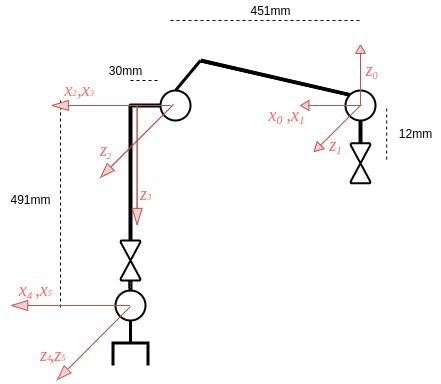
\includegraphics[scale=0.8]{images/dh_configuration.png}
    \legend{Fonte: Autoria própria.}
    \label{fig:dh_config}
\end{figure}

\begin{table}[H]
    \caption{Parâmetros D-H para o manipulador JeRoTIMON.}
    \centering
    \begin{adjustbox}{max width=\textwidth}
    \begin{tabular}{|c|c|c|c|c|}
    \hline
    \rowcolor[HTML]{EFEFEF} 
    Link & a (mm) & $\alpha(^\circ) $ & d (mm) & $\theta(^\circ)$ \\ \hline
    1 & 0   & $90$ & 12  & 0                     \\ \hline
    \rowcolor[HTML]{EFEFEF} 
    2 & 452 & 0         & 0   & $90 - \arctan(30/451)$ \\ \hline
    3 & 30  & $-90$  & 0   & $45 + \arctan(30/451)$ \\ \hline
    \rowcolor[HTML]{EFEFEF} 
    4 & 0   & $90$   & 491 & 0                     \\ \hline
    5 & 0   & 0         & 0   & 0                     \\ \hline
    \end{tabular}
    \end{adjustbox}
    \legend{Fonte: Autoria própria.}
    \label{tab:dh}
    \end{table}



\subsection{Ambiente de operação}
\label{sub:ambiente}

O ambiente físico para a realização do desafio, onde serão incluídos o manipulador e um painel elétrico, é uma mesa com 1.7 m de comprimento por 0.8 m de largura. É necessário então que verifique-se quais os pontos deste ambiente de trabalho que estão dentro da área de alcance (\textit{workspace})\footnote{É a área de alcance do manipulador, região na qual este consegue operar.} do manipulador.

A partir da tabela \ref{tab:dh} foi desenvolvido um código utilizando o software \textit{Matlab R2020a} capaz de gerar pontos que populem o \textit{workspace} do manipulador nas projeções dos planos X-Y, X-Z e Y-Z, conforme exibido nas figuras \ref{fig:workspace_xy}, \ref{fig:workspace_xz} e \ref{fig:workspace_yz}. A região em azul indica o alcance do robô e, a partir destas imagens, é possível observar que o manipulador possui restrições de operação devidas às limitações existentes em cada junta.


% \begin{figure}[H]
%     \caption{Simulação no Gazebo}
%     \centering
%     \includegraphics[scale=0.34]{images/desafio.png}
%     \legend{Fonte: Autoria própria.}
%     \label{fig:simulacao}
% \end{figure}


\begin{figure}[H]
    \caption{\textit{Workspace} do manipulador no plano X-Y.}
    \centering
    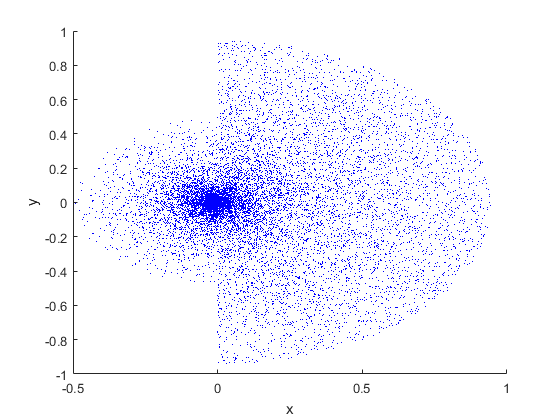
\includegraphics[scale=0.8]{images/workspace_xy.png}
    \legend{Fonte: Autoria própria.}
    \label{fig:workspace_xy}
\end{figure}



\begin{figure}[H]
    \caption{\textit{{Workspace}} do manipulador no plano  X-Z.}
    \centering
    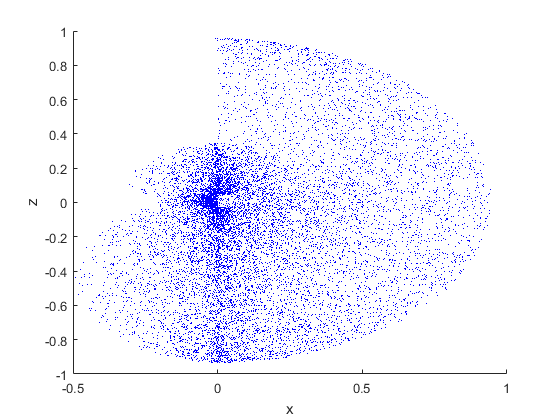
\includegraphics[scale=0.8]{images/workspace_xz.png}
    \legend{Fonte: Autoria própria.}
    \label{fig:workspace_xz}
\end{figure}


\begin{figure}[H]
    \caption{\textit{{Workspace}} do manipulador no plano  Y-Z.}
    \centering
    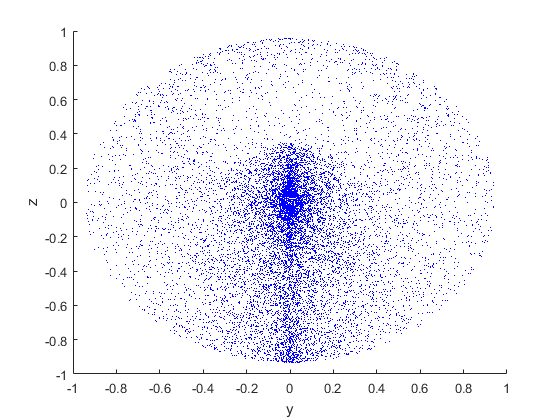
\includegraphics[scale=0.8]{images/workspace_yz.png}
    \legend{Fonte: Autoria própria.}
    \label{fig:workspace_yz}
\end{figure}

\subsection{Estrutura analítica do protótipo}
\label{sub:eap}

A estrutura analítica do protótipo mostrada na Figura \ref{fig:estrutura_analitica} exibe as relações sistemáticas entre as partes que compõem o manipulador. A estrutura hierárquica possui três níveis: o primeiro, referente ao sistema principal JeRoTIMON; o segundo, que é composto pelos sub-sistemas de potência, aquisição, processamento, estrutura e atuação; e o terceiro, composto pelos itens que fazem parte de cada um destes sub-sistemas. 

\begin{figure}[H]
  \caption{Estrutura analítica do protótipo.}
  \centering
  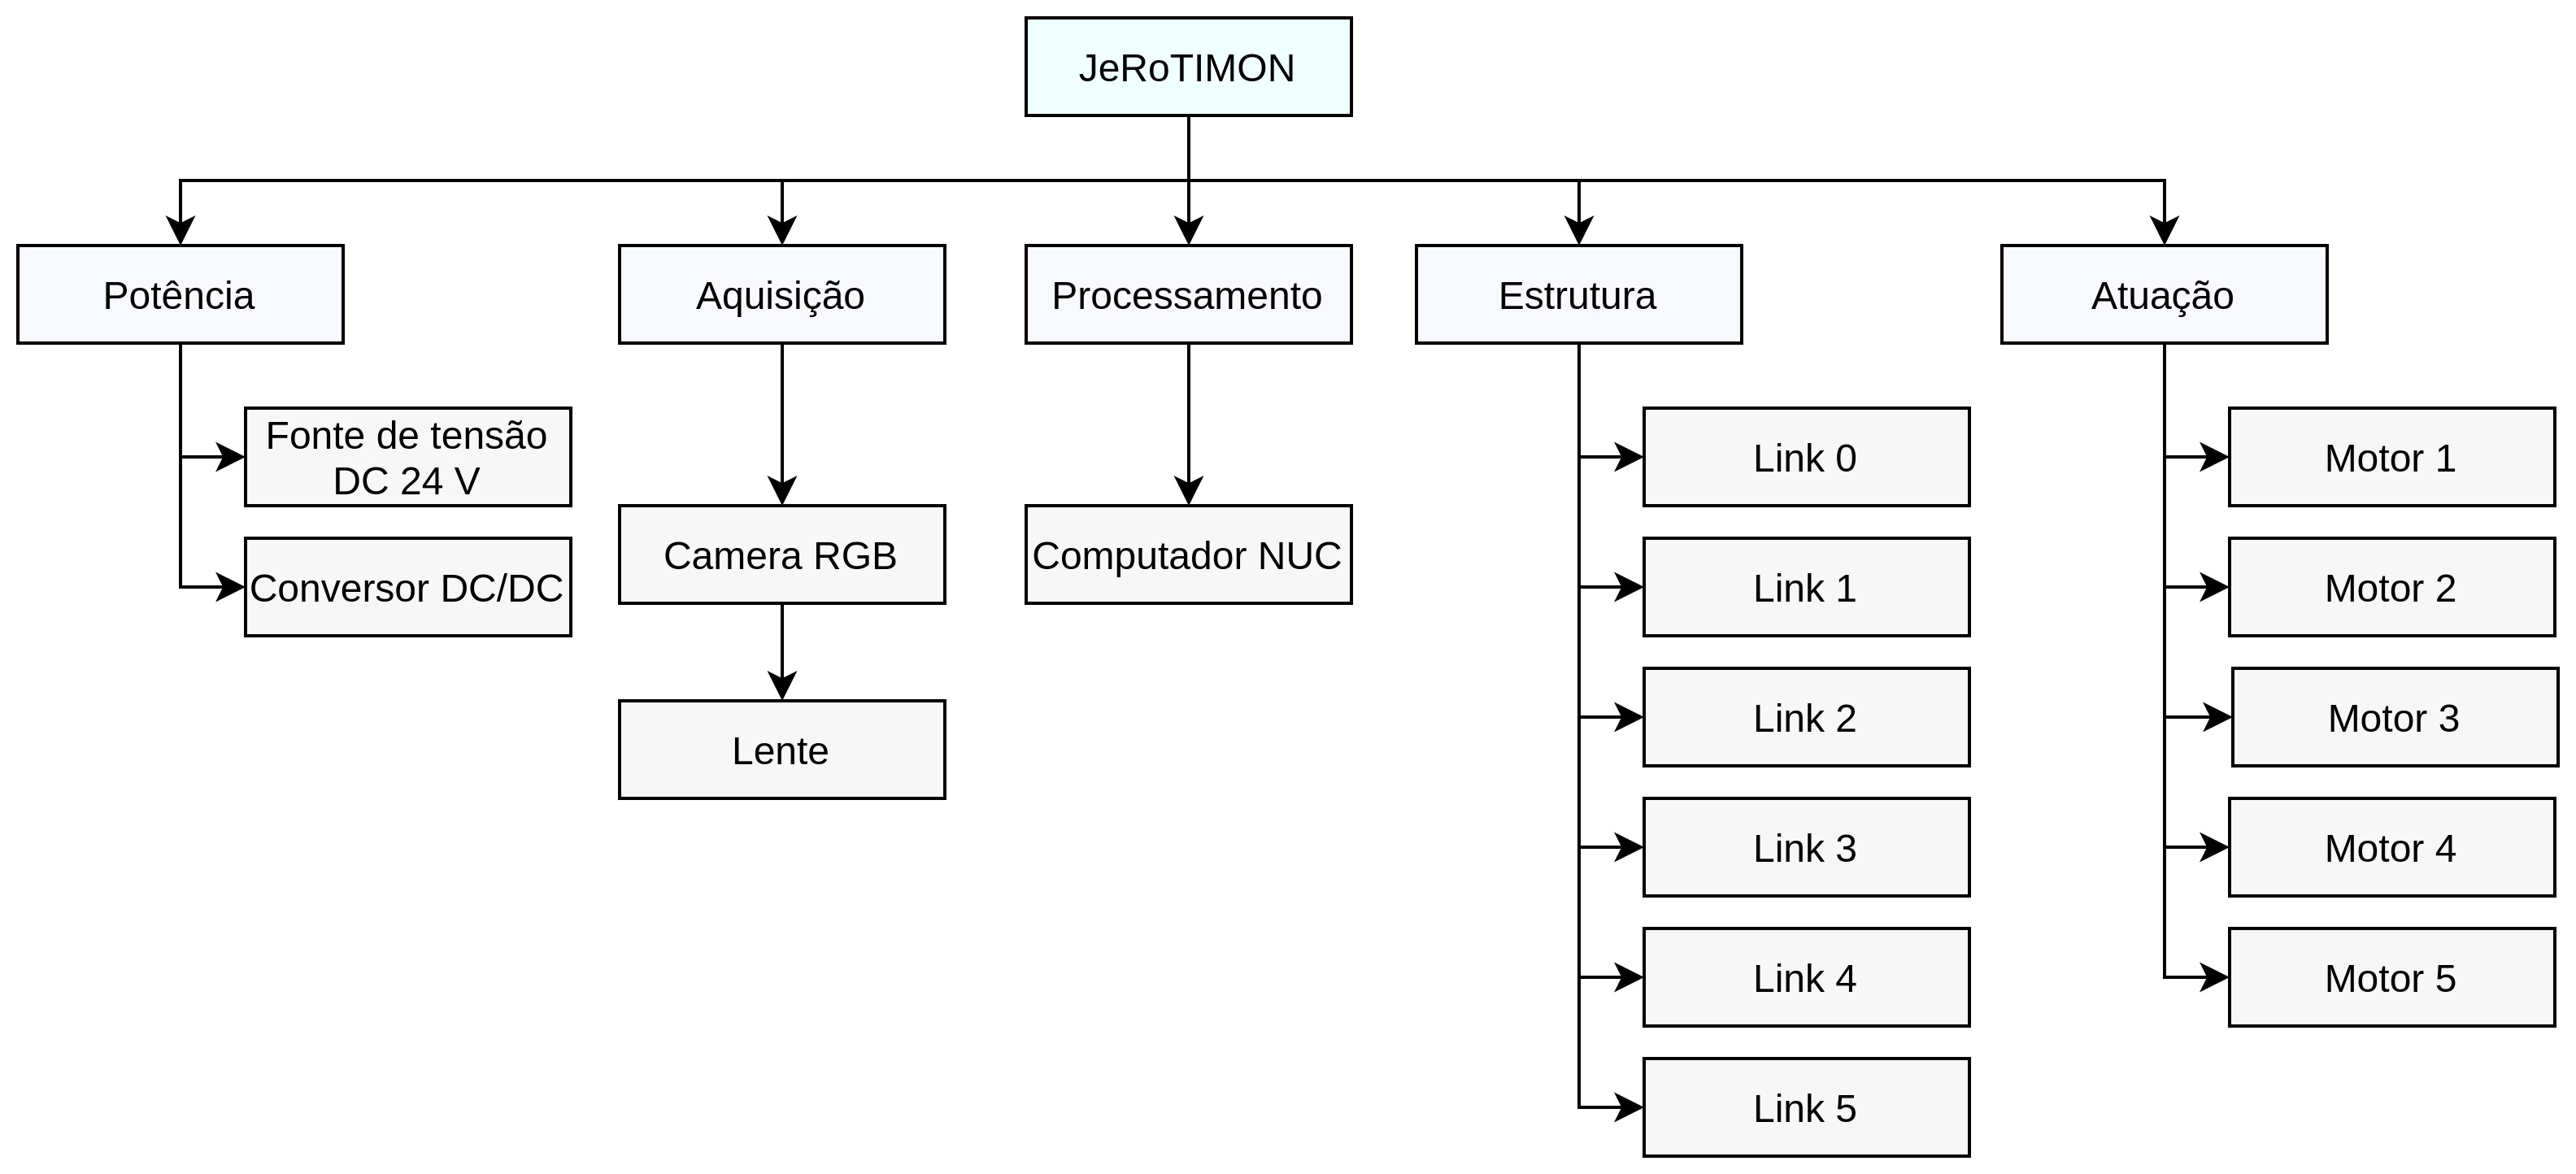
\includegraphics[width=16 cm]{images/estrutura_analitica.jpg}
  \legend{Fonte: Autoria própria.}
  \label{fig:estrutura_analitica}
\end{figure}


%------------------------------------------------------------------
\section{Especificação funcional} %na introdução da seção apresentar a conexão entre as funcionalidades
\label{sec:sota}
O manipulador descrito trabalha acionando os botões encontrados pelo sistema de aquisição. Seu software funciona baseado na troca de mensagens entre duas funcionalidades principais: Escaneamento e Planejamento/Execucção de trajetória. O Escaneamento corresponde à detecção de um marcador visual, que uma vez detectado, informa a posição no espaço de um painel elétrico que precisa ser acionado. O planejamento e execução de trajetória utiliza cálculos de cinemática direta e inversa para definir a trajetória de movimentação que permitirá ao manipulador realizar sua tarefa.


\subsection{Escaneamento}
\label{sub:funcA}

Uma câmera RGB \textit{Teledyne Genie Nano C2590} equipada com lente \textit{kowa LM8FC} foi acoplada ao manipulador JeRoTIMON. Através da mesma é realizada a detecção do marcador visual, utilizando a biblioteca \textit{ArUco} e o pacote \textit{Bir Marker Localization}, hospedado no site do Github no perfil do BIR - Brazilian Institute of Robotics \cite{birmarker}. 

\subsubsection{Descrição} 
\label{ssub:descA}
 
A Figura \ref{fig:flux_vis} exibe o fluxograma que descreve o funcionamento do sistema de escaneamento integrado ao manipulador. Após a captura  da imagem, a partir da câmera RGB, é feito um processamento dos dados obtidos afim de localização da \textit{tag} \textit{ArUco}, cujos tamanho e ID foram previamente estabelecidos. Caso o marcador seja encontrado, as árvores de \textit{TFs} do painel elétrico onde encontra-se o marcador, e do manipulador robótico são conectadas, possibilitando a localização no espaço da pose alvo. Os apêndices \ref{apend:tf1} e \ref{apend:tf2} exibem as árvores de \textit{TFs} antes e após a conexão realizada.

\begin{figure}[!ht]
  \caption{Fluxograma do sistema de escanamento.}
  \centering
  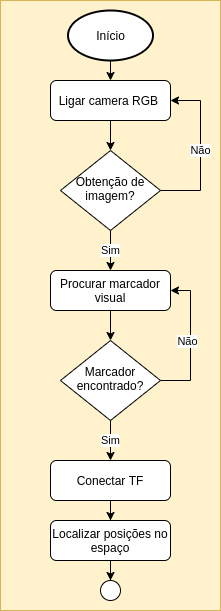
\includegraphics[scale=0.6]{images/fluxograma_sis_vis.png}
  \label{fig:flux_vis}
  \legend{Fonte: Autoria própria.}
\end{figure}


\subsubsection{Premissas necessárias}
\label{ssub:premA}

\begin{itemize}[itemsep=3pt,parsep=3pt]
  \item Conter um marcador visual anexado ao painel elétrico.
  \item A orientação dos elementos envolvidos no escaneamento, câmera RGB e marcador visual, devem ser definidos conforme estabelecido pelo pacote \textit{bir\_marker\_localization}.
  \item Não haver oclusão do marcador visual.
  \item Nível de iluminação do ambiente suficiente para a execução da detecção.
  \item O marcador visual deverá possuir tamanho adequado para detecção.
\end{itemize}

\subsubsection{Dependências}
\label{ssub:depA}

Para realizar a etapa de detecção é necessária a instalação do \textit{\acs{OpenCV}} versão 3.3.1, \textit{driver GigE-V Framework} e a inserção dos pacotes \textit{bir\_marker\_localization} e \textit{def\_cam\_teledyne\_nano} no \textit{workspace} do manipulador.

% \begin{lstlisting}[frame=single]
%   $ git clone git@github.com:Brazilian-Institute-of-Robotics/bir_marker_localization.git
% \end{lstlisting}



\subsubsection{Saídas}
\label{ssub:saidaA}

É fornecida ao sistema resposta por meio de uma sequência de mensagens publicadas no tópico \textit{/timon/camera/image\_raw}. Estes dados são analisados pelo detector \textit{ArUco}, possibilitando seu uso em um pacote desenvolvido na linguagem C++ que determina a posição do painel elétrico associado ao marcador visual. 



\subsection{Planejamento e Execução de Trajetória}
\label{sub:funcB}

As equações cinemáticas são a base que possibilitam a pesquisa do movimento dos manipuladores. A cinemática inversa provê um conjunto de valores para as juntas do manipulador com o intuito de alcançar uma determinada pose pré-estabelecida do seu \textit{endeffector}. Para resolver as equações da cinemática inversa do JeRoTIMON, optou-se por utilizar o plugin TRAC-IK, um método alternativo ao padrão da inversa Jacobiana utilizado pelo \textit{MoveIt}. Este método se adequa bem a manipuladores que possuam limitações em suas juntas, ao contrário de algoritmos baseados no teorema de Newton \cite{beeson2015trac}. Para o planejamento de trajetória foi utilizada a biblioteca \textit{\acs{OMPL}} , uma coleção de algoritmos de planejamento utilizada por padrão no \textit{MoveIt} \cite{sucan2012open}.

\subsubsection{Descrição} 
\label{ssub:descB}

A Figura \ref{fig:flux_pos} exibe o funcionamento do sistema de planejamento e execução de trajetória aplicado ao manipulador. A pose do painel elétrico, determinada a partir do que foi mostrado em \ref{sub:funcA}, é enviada como entrada para o \textit{MoveIt}. Caso seja possível, é realizado o planejamento de uma trajetória para cada uma das juntas do manipulador, a fim de movê-lo para a pose desejada. Esta trajetória é então enviada para os atuadores das juntas, que passam a executá-la. Após a realização da rotina para o pressionamento do painel elétrico, o manipulador retorna para sua posição inicial. Caso alguma condição impeça o planejamento de trajetória, como por exemplo o posicionamento do painel elétrico fora da área de trabalho do manipulador ou falhas nas soluções para as equações da cinemática inversa, uma mensagem de alerta é exibida e o robô realiza uma nova tentativa de planejamento.

\begin{figure}[H]
  \caption{Fluxograma do sistema de planejamento e execução de trajetória.}
  \centering
  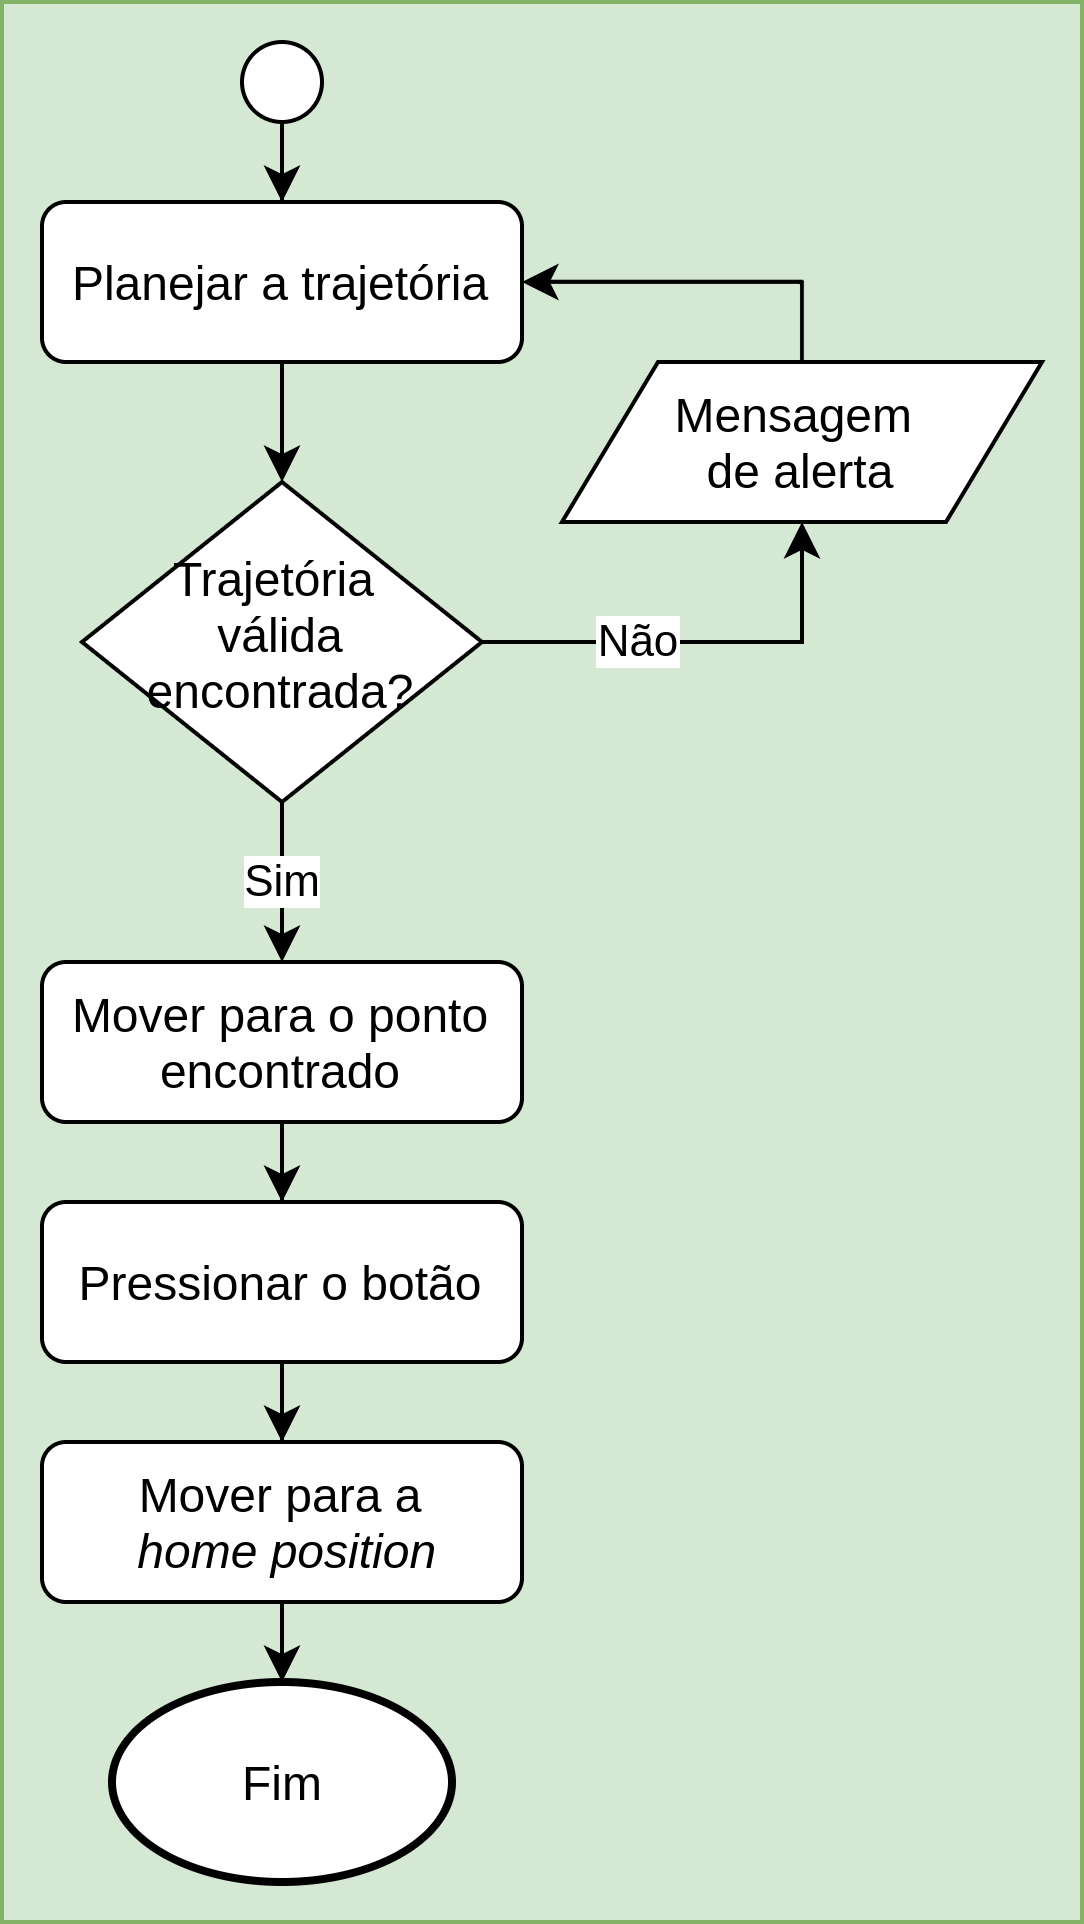
\includegraphics[scale=0.15]{images/fluxograma_plan_traj.png}
  \legend{Fonte: Autoria própria.}
  \label{fig:flux_pos}
\end{figure}
  

\subsubsection{Premissas necessárias}
\label{ssub:premB}
\begin{itemize}
    \item Viabilidade das soluções para cinemática inversa.
    \item Painel elétrico estar posicionado na área de trabalho do manipulador.
\end{itemize}

\subsubsection{Dependências}
\label{ssub:depB}
O sistema de movimentação é dependente da versão Melodic Morenia do \textit{framework} \textit{\acs{ROS}} e da plataforma \textit{MoveIt}. Além destes, uma lista de pacotes deve ser instalada previamente para o funcionamento correto do sistema:

    \begin{itemize}
      \item ros-melodic-ros-control
      \item ros-melodic-gazebo-ros-control
      \item ros-melodic-controller-manager
      \item ros-melodic-joint-trajectory-controller
      \item ros-melodic-joint-state-controller
      \item ros-melodic-position-controllers
      \item ros-melodic-trac-ik-kinematics-plugin
    \end{itemize}

\subsubsection{Saídas}
\label{ssub:saidaB}
As respostas fornecidas pelo sistema de planejamento e execução são publicadas nos  motores \textit{Dynamixel} integrados às juntas do manipulador. A trajetória gerada pelo \textit{MoveIt} pôde ser visualizada a partir do tópico \textit{/move\_group/display\_planned\_path} e é publicada nos motores a partir do tópico \textit{/timon\_arm\_controller/dynamixel\_state}.


%------------------------------------------------------------------
\section{Arquitetura de software}
\label{sec:arqs}
%introdução ao assunto apresentando a arquitetura
O robô JeRoTIMON foi desenvolvido para atuar em conjunto com o \textit{\acs{ROS}}, isto é, segue o propósito de conectar diferentes módulos, como câmeras, motores, sensores e códigos. A proposta é conectar um programa de visão capaz de conectar árvores de TF, através da identificação de marcadores visuais, com um sistema de movimentação que posiciona o manipulador para acionar o painel elétrico.

O apêndice \ref{apend:rqt} exibe o diagrama do \textit{software} do sistema, obtido via \textit{rqt\_graph}. Observa-se a comunicação entre o manipulador (\textit{/timon/robot\_state\_publisher}) e o painel elétrico (\textit{/box/box\_state\_publisher}) a partir da conexão das árvores de \textit{TFs} realizadas pelo \textit{/marker\_localization} que recebe e analisa os dados da câmera (\textit{/timon/camera\_image\_raw}). Pode-se verificar também que o nó \textit{/arm} comunica-se com o nó \textit{/move\_group} e com o nó \textit{/timon\_arm\_controller} a fim de enviar a trajetória planejada pelo \textit{MoveIt} para os motores \textit{dynamixel}.

%\subsection{Diagrama de componentes}
%\label{sub:diagcomp}


%\subsection{Matriz de rastreabilidade de testes}
%\label{sub:matrast}


%------------------------------------------------------------------
\section{Simulação do sistema}
\label{sec:simul}
A simulação do robô JeRoTIMON inserido em seu ambiente de trabalho foi realizada na plataforma \textit{Gazebo}. Para isto, realizou-se o desenvolvimento dos arquivos \textit{timon\_arm.urdf} e \textit{box.urdf}, modelos \textit{\acs{URDF}} que descrevem o robô e o painel elétrico a ser acionado. Foram levados em consideração características de massa, inércia e dimensão para cada componente destes modelos, para que houvesse maior fidelidade possível com o que representam fisicamente, de forma a garantir que os testes realizados possam ser validados em ambiente real. 

O pacote \textit{ros\_control} dispõe de uma lista de controladores disponíveis. Para JeRoTIMON, foram utilizados controladores do tipo \textit{position\_controllers/JointTrajectoryController}, e as transmissões para cada junta do manipulador foram definidas em seu modelo \textit{\acs{URDF}}.

Para simulação dâ câmera RGB, foi desenvolvido o arquivo \textit{camera.xacro}. O plugin padrão do \textit{Gazebo} foi utilizado, \textit{ligazebo\_ros\_camera.so} e as especificações da câmera RGB \textit{Teledyne Genie Nano C2590} foram levados em consideração, garantindo maior realismo à simulação. A figura \ref{fig:timon_gaz} exibe os modelos simulados do manipulador e do painel elétrico, enquanto a figura \ref{fig:camera_gaz} exibe imagem capturada pela câmera instalada no manipulador.


\begin{figure}[H]
  \caption{Modelos simulados do manipulador e do painel elétrico.}
  \centering
  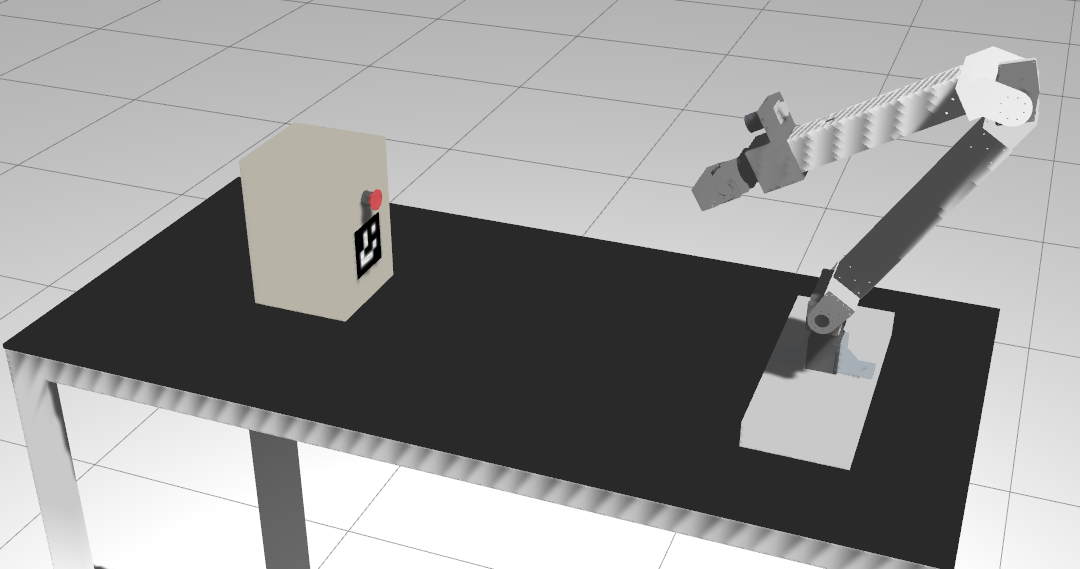
\includegraphics[scale=0.3]{images/timon.png}
  \legend{Fonte: Autoria própria.}
  \label{fig:timon_gaz}
\end{figure}


\begin{figure}[H]
  \caption{Imagem capturada pela câmera RGB.}
  \centering
  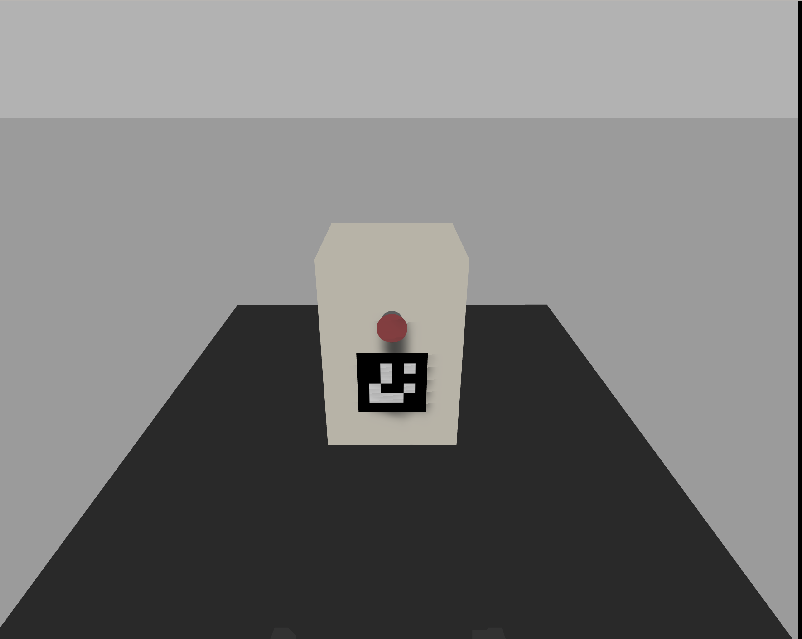
\includegraphics[scale=0.3]{images/camera.png}
  \legend{Fonte: Autoria própria.}
  \label{fig:camera_gaz}
\end{figure}

%\section{Integração}
%\label{sec:integra}






	\chapter{IMPLEMENTAÇÃO}
\label{chap:implementacao}

\section{Parametrização dos motores}
\label{sec:params}

Na Tabela \ref{tab:params_motores} encontram-se as configurações para os motores, que estão identificados na Figura \ref{fig:id_motores}. Nesta Tabela estão especificados os ângulos e as posições mínimas e máximas definidas para cada motor.
Estes parâmetros foram escolhidos após testes e verificações de acordo com a capacidade do manipulador interagir com o ambiente de trabalho, pensando nas possíveis localizações que a caixa poderá estar situada.

% ID1 (min)- angulo $-91$ posição 127113 \\
% ID1 (max)- angulo $90$ posição 127113 \\
% ID2 (min)- angulo $0$ posição 0 \\
% ID2 (max)- angulo $136$ posição 190641 \\
% ID3 (min)- angulo $171$ posição 1955 \\
% ID3 (max)- angulo $281$ posição 3200 \\
% ID5 (min)- angulo $0$ posição 0 \\
% ID5 (max)- angulo $180$ posição 2050 \\
% ID6 (min)- angulo $0$ posição 0 \\
% ID6 (max)- angulo $103$ posição 1174

\begin{figure}[H]
    \centering
    \caption{Identificação dos motores.}
    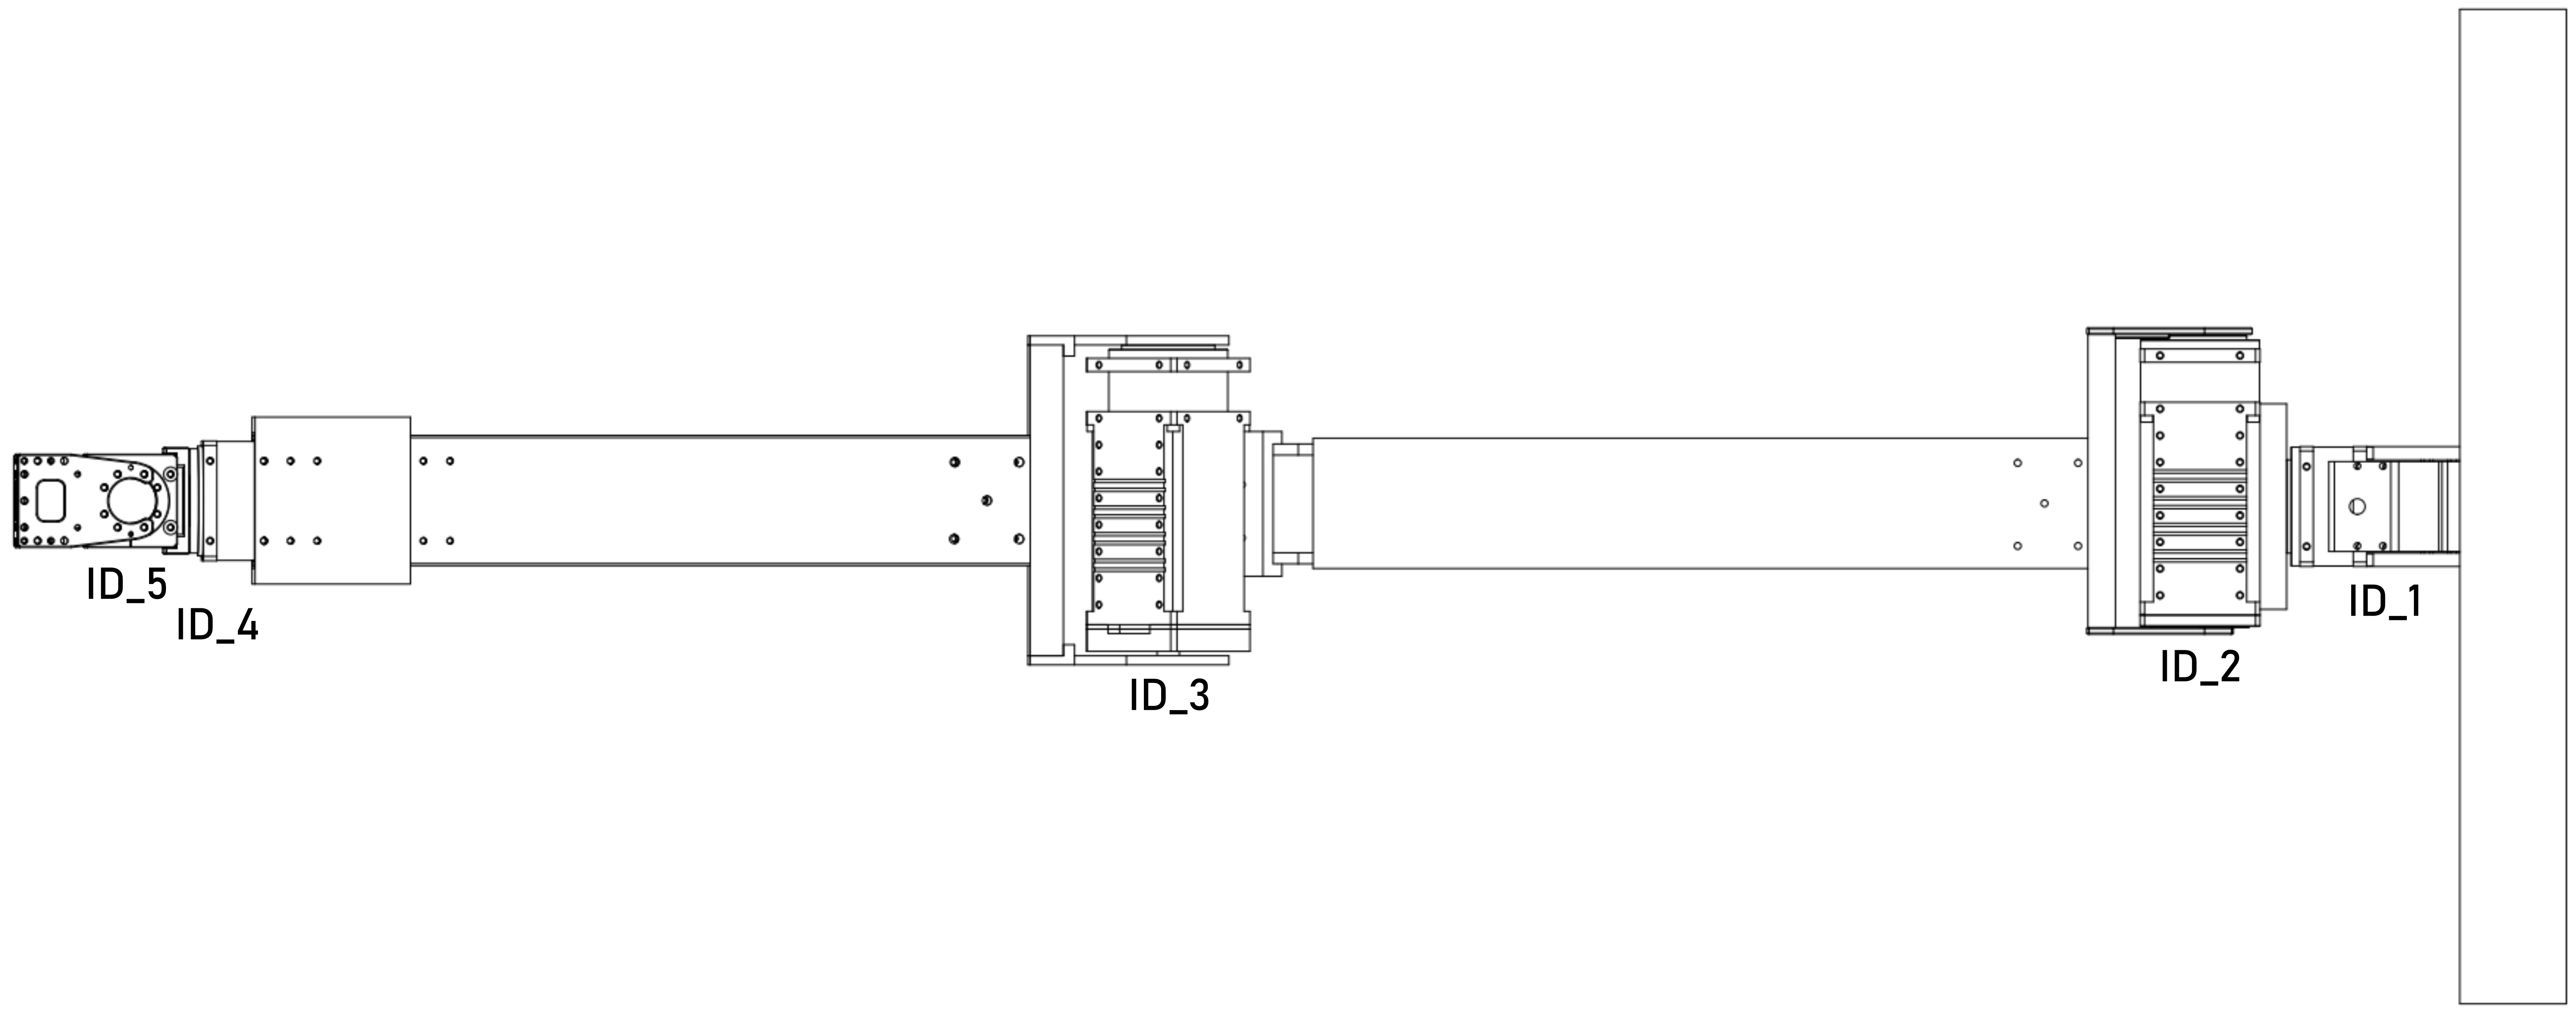
\includegraphics[scale=0.25]{images/id_motores.png}
    \label{fig:id_motores}
    \caption*{Fonte: Autoria própria.}
\end{figure}


\begin{table}[H]
    \centering
    \caption{Parâmetros dos motores.}
    \begin{tabular}{|c|c|c|c|c|}
    \hline
    \rowcolor[HTML]{EFEFEF} 
    Motor & Ângulo (min) & Posição (min) & Ângulo (máx) & Posição (máx) \\ \hline
    \rowcolor[HTML]{FFFFFF} 
    ID\_1 & -$45^\circ$         & -125000       & $45^\circ$         & 125000        \\ \hline
    \rowcolor[HTML]{EFEFEF} 
    ID\_2 & -$90^\circ$         & -250962       & $90^\circ$          & 250962        \\ \hline
    \rowcolor[HTML]{FFFFFF} 
    ID\_3 & -$43^\circ$         & -119095          & $173^\circ$         & 483855          \\ \hline
    \rowcolor[HTML]{EFEFEF} 
    ID\_4 & -$170^\circ$        & -475464       & $170^\circ$         & 475464        \\ \hline
    \rowcolor[HTML]{FFFFFF} 
    ID\_5 & -$90^\circ$         & -151875       & $90^\circ$          & 151875        \\ \hline
    \end{tabular}
    \label{tab:params_motores}
    \caption*{Fonte: Autoria própria.}
\end{table}
%------------------------------------------------------------------

\section{Estrutura física}
Após montagem física, o manipulador obteve um alcance de aproximadamente 980 mm. Levou-se em consideração o mínimo alcance necessário para que a missão possa ser realizada conforme as especificações do cliente. Então foram projetadas cinco juntas rotacionais como mostra a Figura \ref{fig:id_motores}.

\subsection{Base}
Foi decidido utilizar uma base de madeira com dimensões de aproximadamente 450$\times$180 mm e espessura de 50 mm (Figura \ref{fig:base}). Esta base será utilizada para fixar o manipulador, garantindo estabilidade durante a execução da tarefa. 

\begin{figure}[H]
    \centering
    \caption{Base do manipulador.}
    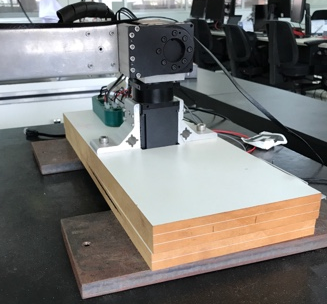
\includegraphics[scale=3]{images/base.png}
    \legend{Fonte: Autoria própria.}
    \label{fig:base}
\end{figure}

%------------------------------------------------------------------

\subsection{Elos ou \textit{links}}
Para estruturação dos elos do robô são utilizados dois perfis de alumínio vazados com comprimento, largura e altura de 350$\times$58.7$\times$58.7 mm, respectivamente (Figuras \ref{fig:elo1} e \ref{fig:elo2}). Estas dimensões foram escolhidas levando em consideração a disponibilidade dos materiais, capacidade de alcance do braço para realizar a tarefa e capacidade estrutural do manipulador, para assim suportar esforços de natureza estática e dinâmica. 

\begin{figure}[H]
    \centering
    \caption{Vista lateral do \textit{link} 2.}
    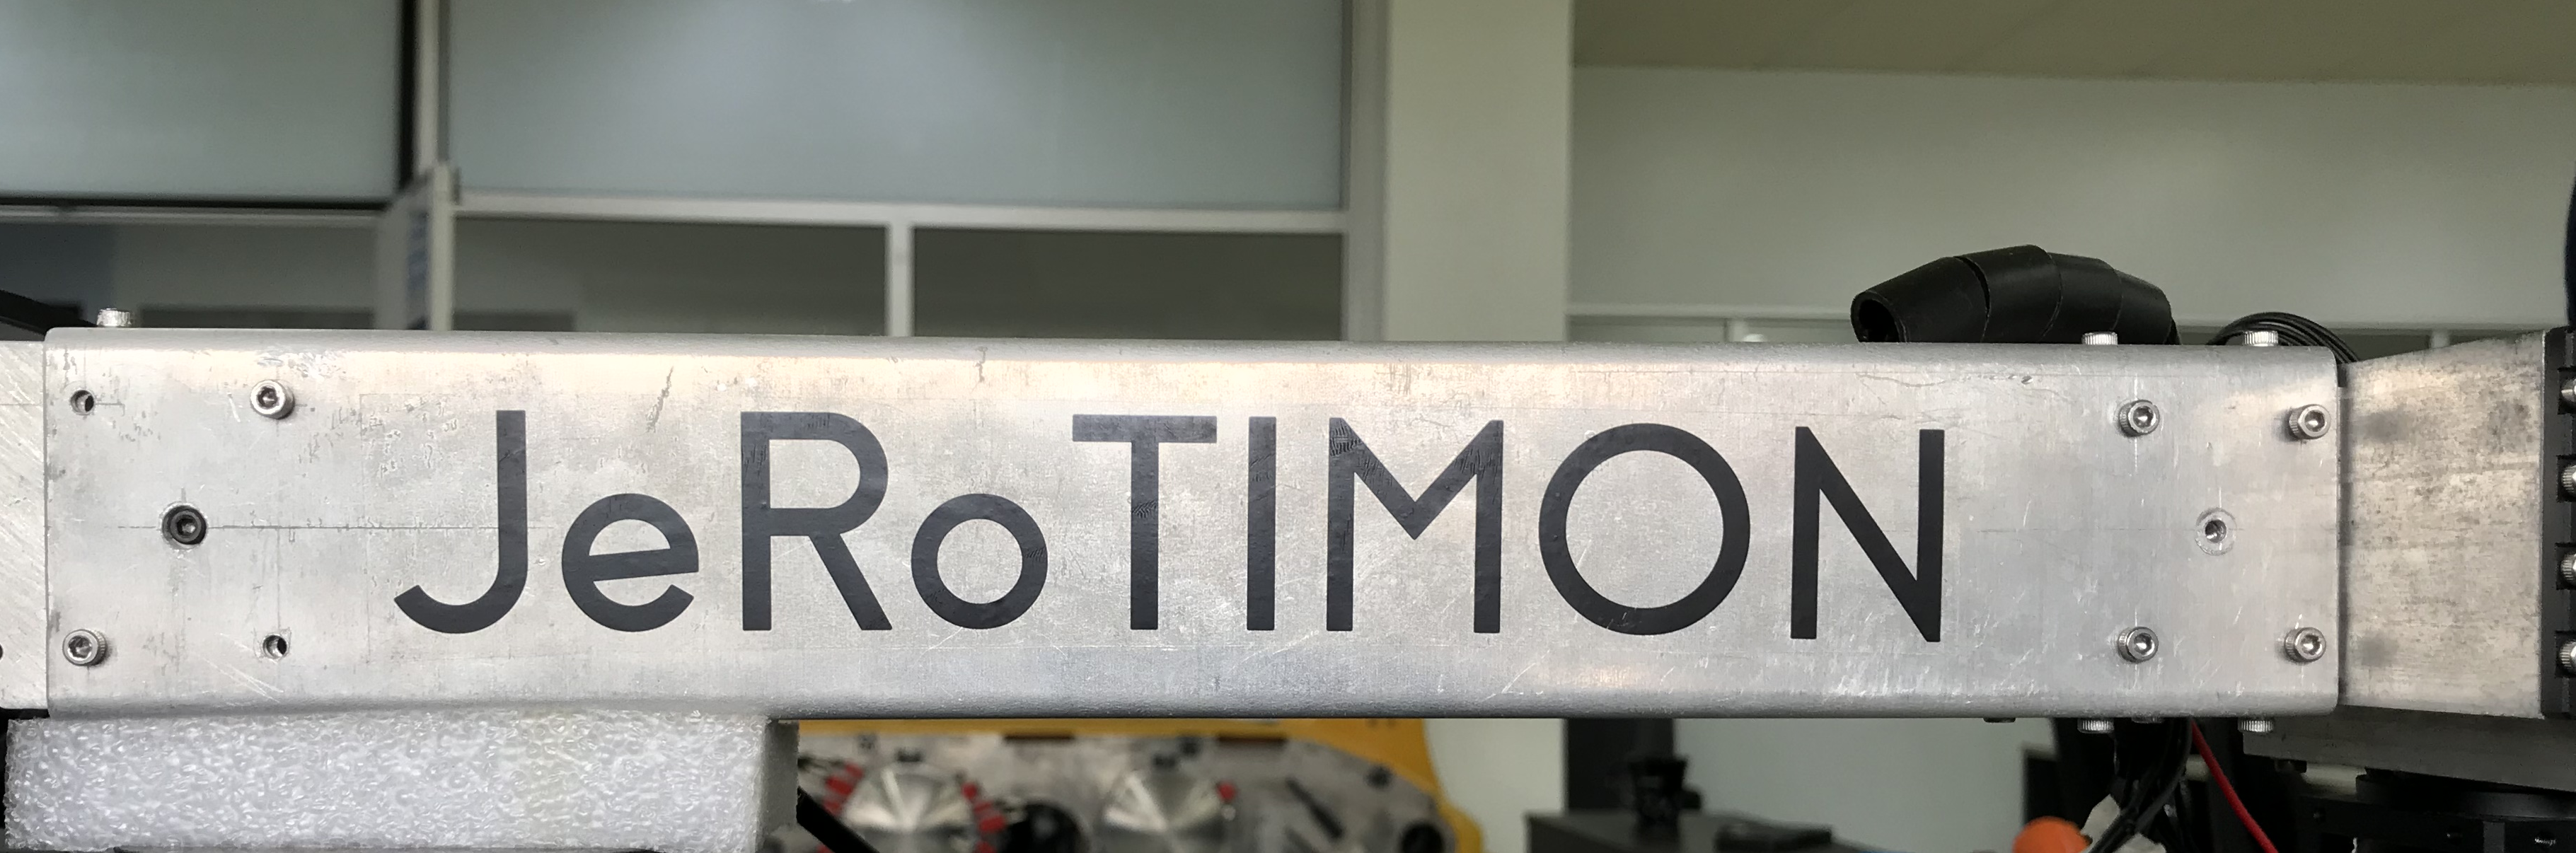
\includegraphics[scale=0.1]{images/elo1.png}
    \legend{Fonte: Autoria própria}
    \label{fig:elo1}
\end{figure}

\begin{figure}[H]
    \centering
    \caption{Vista superior do \textit{link} 2.}
    \includegraphics[scale=0.1]{images/elo2.png}
    \legend{Fonte: Autoria própria}
    \label{fig:elo2}
\end{figure}


%------------------------------------------------------------------

\subsection{Suportes}
Foram utilizados suportes com finalidade de unir os elos do manipulador e distribuir movimentos rotativos para as juntas seguintes, feitos em alumínio. Alguns suportes foram adquiridos através da ROBOTIS, enquanto outros foram confeccionados pelo laboratório CCRoSA. A Tabela com os suportes utilizados e suas imagens e medidas pode ser vista no apêndice \ref{apend:frames}.



%------------------------------------------------------------------
\subsection{Câmera}

Para prover o sistema com capacidade de detecção da \emph{tag} e assim obter dados necessários para aquisição de pose e orientação relativa, utilizou-se uma câmera de vídeo modelo Teledyne Genie Nano C2590 (Figura \ref{fig:genie-nano}) e foi acoplada a lente 16mm C Series VIS-NIR (Figura \ref{fig:lens}). A comunicação entre a câmera e o sistema é feita através de um cabo categoria 6 RJ45, e sua ligação pode ser vista no apêndice \ref{apend:connec_schem}.

\begin{figure}[H]
  \centering
  \caption{Teledyne Genie Nano C2590.}
  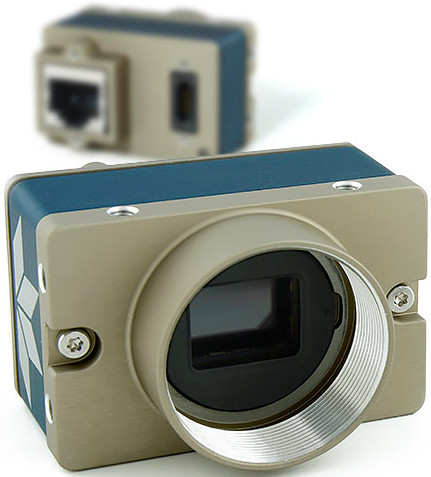
\includegraphics[scale=0.3]{images/genie-nano.jpg}
  \legend{Fonte: \cite{teledyne}}
  \label{fig:genie-nano}
\end{figure}

\begin{figure}[H]
    \centering
    \caption{Lente 16mm C Series VIS-NIR.}
    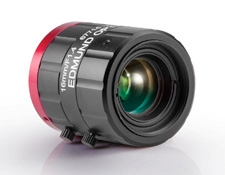
\includegraphics[scale=0.8]{images/lens.png}
    \legend{Fonte: \cite{lens}}
    \label{fig:lens}
\end{figure}

Este conjunto pode ser fixado próxima a extremidade do manipulador robótico utilizando um suporte impresso em ABS (Figura \ref{fig:sup-cam}), facilitando a detecção da \emph{tag} e não comprometendo a estrutura do manipulador. O suporte é conectado ao final do \textit{link} 3, como mostra o apêndice \ref{apend:quest}. A integração pode ser visualizada na Figura \ref{fig:int-sup-cam}.

\begin{figure}[H]
    \centering
    \caption{Suporte para fixação da câmera.}
    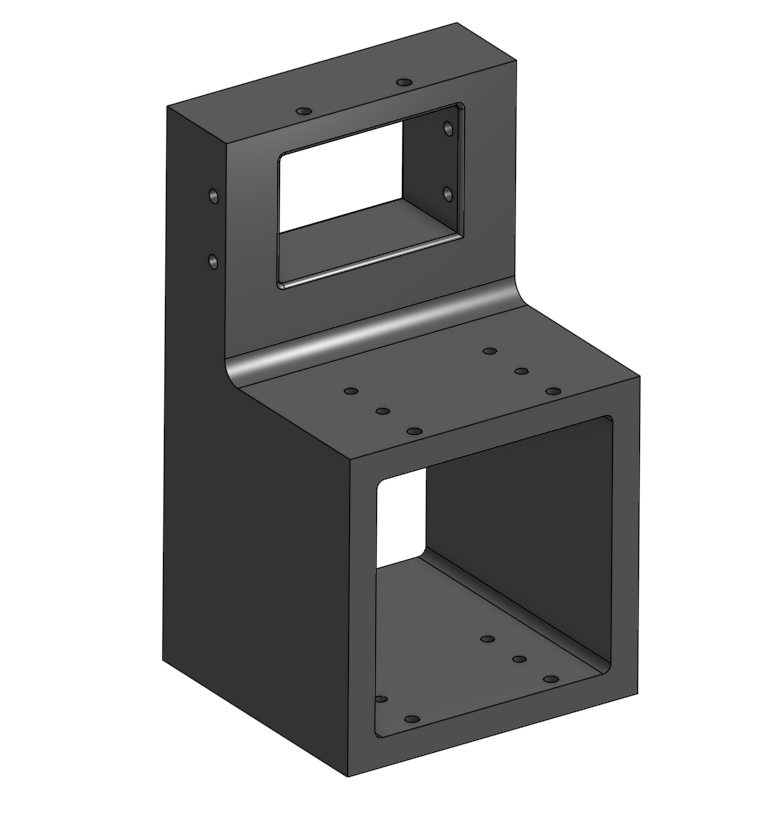
\includegraphics[scale=0.3]{images/sup-cam.png}
    \legend{Fonte: Autoria própria}
    \label{fig:sup-cam}
\end{figure}

\begin{figure}[H]
    \centering
    \caption{Integração suporte-câmera-lente.}
    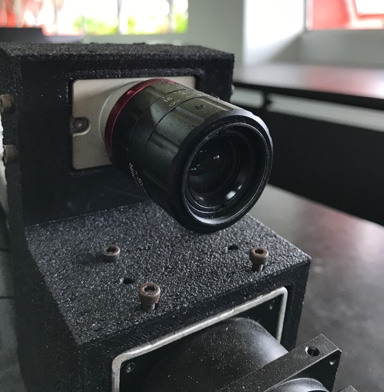
\includegraphics[scale=2.5]{images/cam-sup-int.png}
    \legend{Fonte: Autoria própria}
    \label{fig:int-sup-cam}
\end{figure}



%------------------------------------------------------------------
\subsection{Atuadores}

Os atuadores do manipulador são motores de corrente contínua, integrados com redutor de velocidade, controlador e driver. Foram utilizados atuadores \emph{Dynamixel} da fabricante ROBOTIS. Entre os modelos figuram o PH54-200-S500-R, presente nas juntas 0, 1 e 2, o motor PH54-100-S500-R para a junta 3 e o motor PH42-020-S300-R foi utilizado para a junta 4. As especificações do fabricante mais relevantes no projeto estão apresentadas nas tabelas \ref{tab:specs} e \ref{tab:joints_torque}. As folhas de dados estão disponíveis nos anexos \ref{ann:esp_motors_hp42}, \ref{ann:esp_motors_ph54_100} e \ref{ann:esp_motors_ph54_200} para os atuadores PH42-020-S300-R, PH54-100-S500-R, PH54-200-S500-R, respectivamente.

\begin{table}[H]
    \centering
    \caption{Parâmetros dos motores.}
    \resizebox{\columnwidth}{!}{%
    \begin{tabular}{|c|c|c|c|c|c|}
    \hline
    \rowcolor[HTML]{EFEFEF} 
    Tipo & Torque (N.m) & Tensão (V) & Corrente (A) & Velocidade de Rotação (rpm) & Dimensões (mm) \\ \hline
    \rowcolor[HTML]{FFFFFF} 
    PH54-200-S500-R & 44.7 & 24.0 & 9.3 & 29.0 & 54.0 X 126.0 X 54.0 \\ \hline
    \rowcolor[HTML]{EFEFEF} 
    PH54-100-S500-R & 25.3 & 24.0 & 5.5 & 29.2 & 54.0 X 108.0 X 54.0 \\ \hline
    \rowcolor[HTML]{FFFFFF} 
    PH42-020-S300-R & 5.1 & 24.0 & 1.5 & 29.2 & 42.0 X 84.0 X 42.0 \\ \hline
    \end{tabular}
    }

    \label{tab:specs}
    \caption*{Fonte: \cite{dynamixel}}
\end{table}

%------------------------------------------------------------------
\section{Sistema de Potência}
O sistema necessitará ser energizado em dois níveis de tensão, 12 V e 24 V. Durante a realização dos testes, utilizou-se uma fonte com níveis de tensão de 0-30 V e fornecimento de corrente de 0-10 A, para atender os requisitos necessários de potência dos motores. Foi utilizado um conversor DC-DC modelo UWE-12/10-Q12PB-C (Figura \ref{fig:dcdcimg}) na saída da fonte para atingir o nível de tensão de 12 V e energizar a câmera. Um esquema elétrico é fornecido no apêndice \ref{apend:diag_ele}, indicando as conexões dos cabos entre os motores e a câmera.

\begin{figure}[H]
    \centering
    \caption{UWE-12/10-Q12PB-C.}
    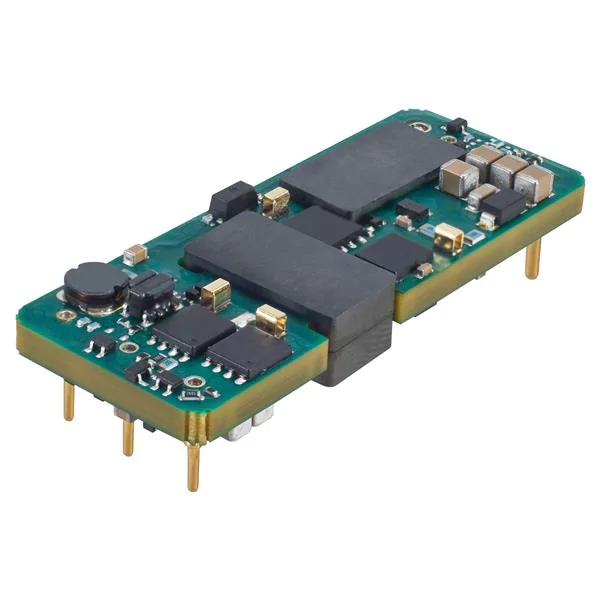
\includegraphics[scale=0.20]{images/dcdc.png}
    \legend{Fonte: \cite{dcdc}}
    \label{fig:dcdcimg}
\end{figure}

\section{Comunicação}

O manipulador é conectado via USB através de um disposivo denominado U2D2 \cite{u2d2}. Ele consegue parametrizar e enviar comandos para os motores através dos \textit{softwares} originais da ROBOTIS chamados Dynamixel Workbench e Dynamixel Wizard. O padrão elétrico utilizado é RS-485, ou seja, utiliza-se de 4 fios de conexão que transmitem níveis de tensão e dados. A conexão de entre o computador e os motores, utilizando o U2D2 de intermédio, pode ser vista no apêndice \ref{apend:connec_schem}. A velocidade de transmissão (\textit{baud rate}) definida para todos os motores no sistema é de 57600 bps.

\begin{figure}[H]
    \centering
    \caption{U2D2.}
    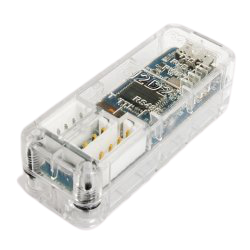
\includegraphics[scale=0.70]{images/u2d2.png}
    \legend{Fonte: \cite{u2d2}}
    \label{fig:u2d2img}
\end{figure}


\section{Análise de esforços}
A análise de esforços mecânicos aos quais o manipulador está exposto foi realizada para embasamento e confirmação da capacidade da estrutura e dos atuadores suportarem os esforços de momento torsor. Para isso foram analisadas individualmente as juntas em seus estados críticos. Na Tabela \ref{tab:joints_torque} é apresentada a análise de esforços nas juntas e comparados com os máximos esforços suportados pelos atuadores (conforme vistos nos apêndices \ref{ann:esp_motors_hp42}, \ref{ann:esp_motors_ph54_100} e \ref{ann:esp_motors_ph54_200}), para evitar falhas mecânicas.

Levando em consideração os valores obtidos nas análises de esforços, tem-se as juntas 0 e 1 como juntas críticas do sistema, pois elas sofrem a maior força do sistema e tem o maior torque exigido. Na configuração apresentada, as juntas 0 e 1 suportam a carga máxima de 45.22 N sem chegar a falha mecânica, logo o manipulador possui um limite (\emph{payload}) de aproximadamente 2.1 kg na sua extremidade.

\begin{table}[H]
    \centering
    \caption{Torque das juntas.}
    \resizebox{\columnwidth}{!}{%
    \begin{tabular}{|c|c|c|c|}
    \hline
    \rowcolor[HTML]{EFEFEF} 
    \textbf{Junta} & \textbf{\begin{tabular}[c]{@{}c@{}}Torque máximo fornecido \\ pelos motores (Nm)\end{tabular}} & \textbf{Força resultante na junta (N)} & \textbf{Torque exigido pela junta (Nm)} \\ \hline
    0              & 44.7                                                                                           & 45.22                                  & 25.8                                    \\ \hline
    \rowcolor[HTML]{EFEFEF} 
    1              & 44.7                                                                                           & 45.22                                  & 25.8                                    \\ \hline
    2              & 44.7                                                                                           & 21.44                                  & 6.9                                     \\ \hline
    \rowcolor[HTML]{EFEFEF} 
    3              & 25.3                                                                                           & 4.8                                    & 0.12                                    \\ \hline
    4              & 5.1                                                                                            & 0.87                                   & 0.05                                    \\ \hline
    \end{tabular}
    }
    \label{tab:joints_torque}
    \caption*{Fonte: Autoria própria.}
\end{table}
%------------------------------------------------------------------
%------------------------------------------------------------------
\section{Configurações}
\label{sec:configuracoes}

O conjunto formado pelo manipulador, seu espaço de trabalho e os objetos com os quais ele deverá interagir compõem o sistema abordado neste trabalho. O espaço de trabalho foi representado como uma bancada de 1.70 m $\times$ 0.80 m $\times$ 0.028 m. Há apenas um objeto com o qual o manipulador deverá interagir, uma caixa de dimensões 0.30 m $\times $0.20 m $\times$ 0.20 m.

Para o desafio foi utilizado um marcador visual \textit{ArUco} com dimensões 58x58 mm de id 4, conforme mostrado na Figura \ref{fig:box-real}. Este tem 8 cm do centro do \textit{ArUco} para o botão e 7 cm do centro do \textit{ArUco} para a lâmpada, esta identifica se o botão foi acionado ou não pelo manipulador. 

\begin{figure}[H]
    \centering
    \caption{Caixa objetivo.}
    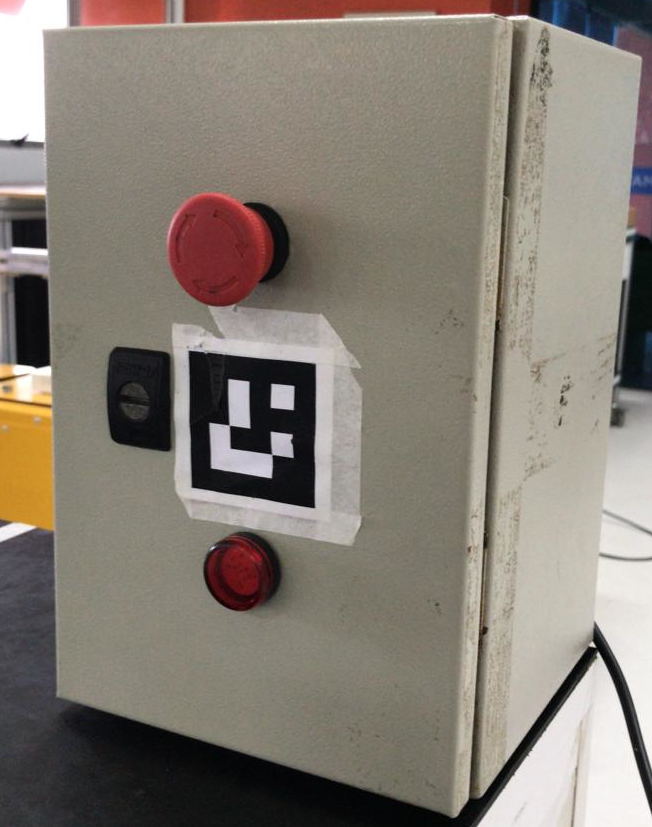
\includegraphics[scale=1.8]{images/box-real.png}
    \legend{Fonte: Autoria própria}
    \label{fig:box-real}
\end{figure}



O manipulador possui a posição home definida como da Figura \ref{fig:home_position} onde o ângulo de cada motor está descrito na Tabela \ref{tab:home_position}.

\begin{figure}[H]
    \centering
    \caption{Manipulador na posição home.}
    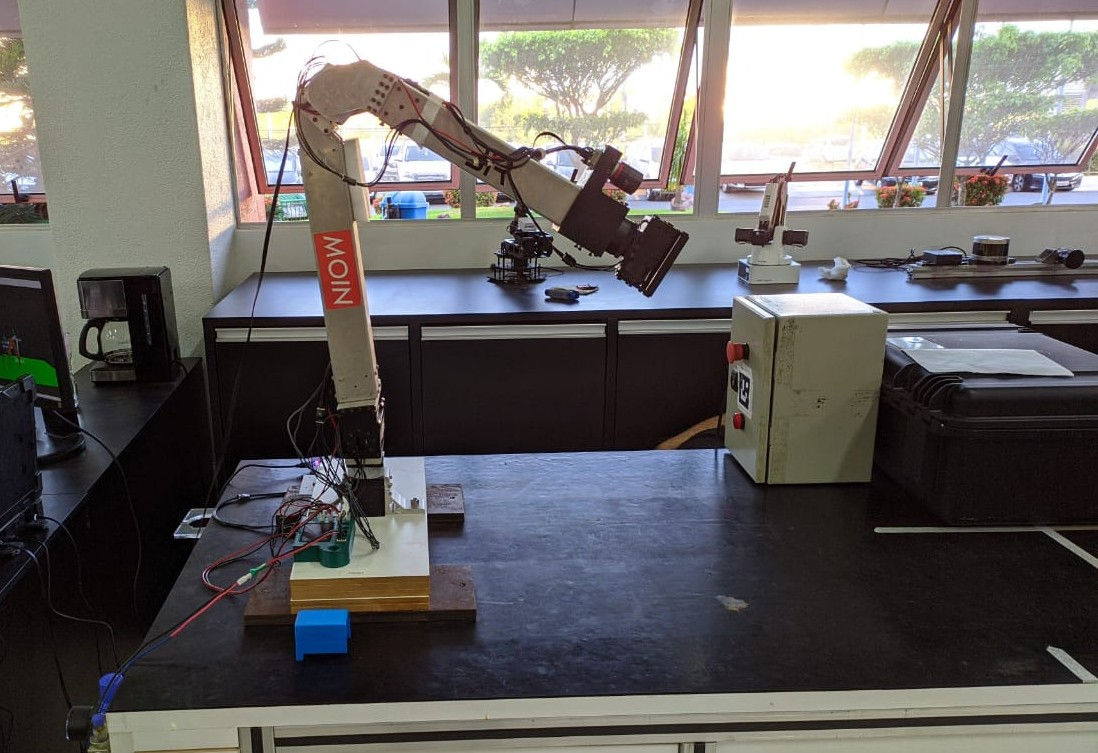
\includegraphics[scale=0.4]{images/home_position.jpg}
    \label{fig:home_position}
    \caption*{Fonte: Autoria própria.}
\end{figure}

\begin{table}[H]
    \centering
    \caption{Ângulos dos motores na posição home.}
    \begin{tabular}{|c|c|}
    \hline
    \rowcolor[HTML]{EFEFEF} 
    \textbf{Motor} & \textbf{Ângulo}                           \\ \hline
    \rowcolor[HTML]{FFFFFF} 
    ID\_1          & $0^\circ$   \\ \hline
    ID\_2          & $-24^\circ$ \\ \hline
    \rowcolor[HTML]{FFFFFF} 
    ID\_3          & $141^\circ$ \\ \hline
    ID\_4          & $0^\circ$   \\ \hline
    \rowcolor[HTML]{FFFFFF} 
    ID\_5          & $0^\circ$   \\ \hline
    \end{tabular}
    \label{tab:home_position}
    \caption*{Fonte: Autoria própria.}
    \end{table}



	\chapter{RESULTADOS E ANÁLISES}
\label{chap:result}

Os experimentos apresentados nesta seção possuem como objetivo avaliar o desempenho do manipulador robótico desenvolvido.

\section{Caracterização do problema e determinação do modelo}

Para análise da performance do manipulador, deseja-se avaliar inicialmente a interação de algumas variáveis que podem influenciar no desempenho do manipulador. Em um segundo momento, após estabelecidas as melhores configurações de algoritmo e velocidade para o robô, os testes devem seguir uma análise de repetibilidade e de variância do sistema.

No planejamento dos experimentos, foram levantadas quais variáveis seriam de interesse para avaliar a performance do robô, com isso foram selecionadas como variáveis de saída a precisão do manipulador, ou seja, a capacidade do mesmo de chegar a uma posição determinada com o menor erro possível, tempo de busca do marcador visual,  e o tempo necessário para o acionamento do botão (missão imposta ao manipulador). 

Também foram selecionadas as variáveis independentes, ou seja, as variáveis de entrada do processo, que serão analisadas quanto às suas influências no sistema de forma isolada ou a interação entre as mesmas. As variáveis selecionadas para o estudo foram: velocidade de operação dos motores, algoritmo de planejamento de trajetória utilizado e a posição da caixa no ambiente de trabalho do manipulador. 

\section{Planejamento dos experimentos}

Definido o problema e as variáveis a serem estudadas, foi realizado um planejamento dos experimentos, para assim gerar dados e resultados confiáveis acerca da melhor configuração para o manipulador. As tabelas \ref{tab:tabexp1}, \ref{tab:tabexp2} e \ref{tab:tabexp3} apresentam os modelos dos experimentos. 

\begin{table}[h!]
  \centering
  \caption{Modelo de experimentos para análise de 3 variáveis.}
  \scalebox{0.8}{%
  \begin{tabular}{|
    >{\columncolor[HTML]{EFEFEF}}c |
    >{\columncolor[HTML]{EFEFEF}}c |
    >{\columncolor[HTML]{EFEFEF}}c |
    >{\columncolor[HTML]{EFEFEF}}c |}
    \hline
    \textbf{\begin{tabular}[c]{@{}c@{}}Variáveis \\ Independentes\end{tabular}} & \multicolumn{2}{c|}{\cellcolor[HTML]{EFEFEF}\textbf{Níveis}} & \textbf{Variáveis dependentes} \\ \hline
    \cellcolor[HTML]{FFFFFF} & \cellcolor[HTML]{FFFFFF} & \cellcolor[HTML]{FFFFFF} & \cellcolor[HTML]{FFFFFF} \\
    \multirow{-2}{*}{\cellcolor[HTML]{FFFFFF}\begin{tabular}[c]{@{}c@{}}Algoritmo de planejamento\\ de trajetória\end{tabular}} & \multirow{-2}{*}{\cellcolor[HTML]{FFFFFF}RRT-CONNECT} & \multirow{-2}{*}{\cellcolor[HTML]{FFFFFF}Kpiece} & \multirow{-2}{*}{\cellcolor[HTML]{FFFFFF}Erro de posição} \\ \hline
    Velocidade dos motores & 300 & 500 & \cellcolor[HTML]{EFEFEF} \\ \cline{1-3}
    Posição da caixa & A & B & \multirow{-2}{*}{\cellcolor[HTML]{EFEFEF}Tempo total} \\ \hline
\end{tabular}}
\label{tab:tabexp1}
\legend{Fonte: Autoria própria.}
\end{table}


\begin{table}[h!]
  \centering
  \caption{Modelo de experimentos ANOVA sem detecção da \textit{tag}.}
  \scalebox{0.8}{%
  \begin{tabular}{|
    >{\columncolor[HTML]{EFEFEF}}c |
    >{\columncolor[HTML]{EFEFEF}}c |
    >{\columncolor[HTML]{EFEFEF}}c |}
    \hline
    \textbf{Ponto} & \textbf{Número de repetições} & \textbf{Variáveis dependentes} \\ \hline
    \cellcolor[HTML]{FFFFFF} & \cellcolor[HTML]{FFFFFF} & \cellcolor[HTML]{FFFFFF} \\
    \multirow{-2}{*}{\cellcolor[HTML]{FFFFFF}A} & \multirow{-2}{*}{\cellcolor[HTML]{FFFFFF}10} & \multirow{-2}{*}{\cellcolor[HTML]{FFFFFF}Erro de posição} \\ \hline
    B & 10 & Erro de posição \\ \hline
  \end{tabular}}
  \label{tab:tabexp2}
  \legend{Fonte: Autoria própria.}
  \end{table}

\begin{table}[h!]
  \centering
  \caption{Modelo de experimentos ANOVA com detecção da \textit{tag}}
  \scalebox{0.8}{%
  \begin{tabular}{|c|c|c|c|c|}
    \hline
    \rowcolor[HTML]{EFEFEF} 
    \textbf{Operador} & \textbf{Pose da caixa} & \textbf{Número de reptições} & \textbf{Sucesso} & \textbf{Variáveis dependentes} \\ \hline
    \rowcolor[HTML]{FFFFFF} 
    1 & A & 10 & -1,1 & Erro de posição \\ \cline{1-4}
    \rowcolor[HTML]{EFEFEF} 
    2 & B & 10 & -1,1 & Tempo de busca \\ \cline{1-4}
    \rowcolor[HTML]{FFFFFF} 
    1 & B & 10 & -1,1 & Tempo total \\ \cline{1-4}
    \rowcolor[HTML]{EFEFEF} 
    2 & A & 10 & -1,1 &  \\ \hline
    \end{tabular}}
    \label{tab:tabexp3}
    \legend{Fonte: Autoria própria.}
  \end{table}

%------------------------------------------------------------------

\newpage

\section{Resultados alcançados}
\label{sec:resalcanc}
A partir dos testes realizados sob orientação do planejamento, foram coletados os resultados do tempo de busca do marcador visual, tempo da missão do manipulador e o erro de posição em cada experimento. As amostras dos testes coletadas foram analisados da seguinte forma: Análise de regressão linear, análise de variância e teste R\&R, para os testes com e sem a detecção do marcador visual . 

\subsection{Análise de regressão linear}
A partir do planejamento de experimentos realizados, foram tomados três dados de cada condição estabelecida e utilizada a média entre os três resultados como valor do experimento. As amostras coletadas estão representadas na tabela \ref*{tab:reg}. O  algoritmo de planejamento RRT CONNECT é representado pelo sinal de subtração (-) enquanto o sinal de adição (+) representa o algoritmo Kpiece. Já para as velocidades, (+) representa o valor de 500 rpm e (-) representa 300 rpm.
\begin{table}[h!]
  \centering
  \caption{Resultados das amostras coletadas.}
  \scalebox{0.9}{%
  \begin{tabular}{|c|c|c|c|c|}
    \hline
    \rowcolor[HTML]{EFEFEF} 
    \textbf{Ordem} & \textbf{Algoritmo} & \textbf{Velocidade} & \textbf{Erro} & \textbf{Tempo} \\ \hline
    \rowcolor[HTML]{FFFFFF} 
    1 & - & - & 0.0004759353 & 175.25667 \\ \hline
    \rowcolor[HTML]{EFEFEF} 
    2 & + & - & 0.0009316073 & 82.24667 \\ \hline
    \rowcolor[HTML]{FFFFFF} 
    3 & - & + & 0.0002889380 & 139.39333 \\ \hline
    \rowcolor[HTML]{EFEFEF} 
    4 & + & + & 0.0008311057 & 90.34333 \\ \hline
    \end{tabular}}
    \label{tab:reg}
    \legend{Fonte: Autoria própria.}
  \end{table}
 
O resultado obtido a partir da análise linear aplicada aos dados é disposto na tabela \ref*{tab:reg2}. O primeiro modelo dessa análise pode ser visualizado na Equação \ref*{eq:model1}.  Esta equação mostra um modelo que consegue explicar o valor do erro de posição a partir da relação entre os parâmetros.


\begin{table}[h!]
  \centering
  \caption{Resultados da análise de regressão linear.}
  \scalebox{0.9}{%
  \begin{tabular}{|c|c|c|c|c|}
    \hline
    \rowcolor[HTML]{EFEFEF} 
    \textbf{} & \textbf{Estimate Std.} & \textbf{Error} & \textbf{t value} & \textbf{Pr(\textgreater{}|t|)} \\ \hline
    \rowcolor[HTML]{FFFFFF} 
    (Intercept) & 4.543e-04 & 3.745e-05 & 12.130 & 0.0524 \\ \hline
    \rowcolor[HTML]{EFEFEF} 
    algoritmo+ & 4.989e-04 & 4.325e-05 & 11.536 & 0.0550 \\ \hline
    \rowcolor[HTML]{FFFFFF} 
    velocidade+ & -1.437e-04 & 4.325e-05 & -3.324 & 0.1860 \\ \hline
    \end{tabular}}
    \label{tab:reg2}
    \legend{Fonte: Autoria própria.}
  \end{table}

\begin{align}
    \begin{split}
    erro &= 4.543.(10^{-04}) + 4.989.(10^{-04})  \text{.algoritmo(+)} - 1.437.(10^{-04})  \text{.velocidade(+)}
    \end{split}
    \label{eq:model1}
\end{align}

Observando os dados apresentados na tabela \ref*{tab:reg2}, o $\rho$-valor da variável velocidade é superior a 0,05, aceitando a hipótese nula, ou seja, a variável velocidade possui pouca ou nenhuma influência na tomada de dados do sistema. Porém, percebe-se que o $\rho$-valor da variável algoritmo é próxima de 0.05, implicando que a mesma pode ser analisada de forma individual, rejeitando-se a hipótese nula para esta variável. Desta forma refazendo-se a análise linear do erro de posição com relação apenas a variável algoritmo obtém-se o novo modelo representado na equação \ref*{eq:model2}. O resultado dos coeficientes pode ser visto na tabela \ref*{tab:reg3}.

\begin{table}[h!]
  \centering
  \caption{Resultados da análise de regressão linear (variável algoritmo).}
  \scalebox{0.9}{%
  \begin{tabular}{|c|c|c|c|c|}
    \hline
    \rowcolor[HTML]{EFEFEF} 
    \textbf{} & \textbf{Estimate Std.} & \textbf{Error} & \textbf{t value} & \textbf{Pr(\textgreater{}|t|)} \\ \hline
    \rowcolor[HTML]{FFFFFF} 
    (Intercept) & 3.824e-04 & 7.506e-05 & 5.095 & 0.0364 \\ \hline
    \rowcolor[HTML]{EFEFEF} 
    algoritmo+ & 4.989e-04 & 1.062e-04 & 4.700 & 0.0424 \\ \hline
    \end{tabular}}
    \label{tab:reg3}
    \legend{Fonte: Autoria própria.}
  \end{table}

\begin{align}
    \begin{split}
    erro &= 3.824.(10^{-04}) + 4.989.(10^{-04})  \text{.algoritmo(+)}
    \end{split}
    \label{eq:model2}
\end{align}

Como apresentado na tabela \ref*{tab:reg3} o algoritmo apresenta $\rho$-valor menor que 0.05, ou seja, rejeita-se a hipótese nula para esta variável, mostrando que a mesma tem influência no erro de posição do manipulador. 

Após esta análise serão realizados novos testes levando em consideração as variáveis examinadas neste estudo, sendo configurado o sistema com o algoritmo RRT CONNECT, uma vez que o algoritmo Kpiece teve influência positiva, ou seja, aumentou o erro de posição do manipulador, o que não é desejável para este sistema. A velocidade dos motores não apresentou influência considerável nos testes, portanto foi configurada com a menor velocidade por motivos de segurança.

\subsection{ANOVA}

Com o algoritmo de planejamento e velocidade estabelecidas para a continuidade dos testes, foram realizados dois tipos de experimentos: análise de erro de posição do \textit{end-effector} sem a detecção do marcador visual, ou seja, o manipulador recebe comandos de posição em x, y e z dentro da sua área de trabalho e então é observado o erro ao executar o comando de posição. O segundo teste foi semelhante, porém, este contou com a detecção da \textit{tag}, recebendo assim o comando de posição a partir da detecção do marcador visual. Com isso foram tomados dados em duas diferentes poses para assim analisar a variância do erro em cada pose e entre elas. 

\subsubsection{Análise de variância sem detecção da \textit{tag}}

Para esta análise foram estabelecidas, na área de trabalho do manipulador, duas posições, onde Pose A equilave a x = 0.314445 y = 0.730867 z = 0.233471 e Pose B equilave a x = -0.153158 y = 0.755479 z = 0.238906, ambas referentes ao \textit{endeffector} do manipulador, e então foram realizados 10 execuções de movimento para cada pose estabelecida. A tabela \ref*{tab:anova1} mostra os erros de posição do \textit{endeffector} para cada uma das execuções.

\begin{table}[h!]
  \centering
  \caption{Resultados dos experimentos sem detecção da \textit{tag}.}
  \scalebox{0.9}{%
  \begin{tabular}{|c|c|c|}
    \hline
    \rowcolor[HTML]{EFEFEF} 
    \textbf{} & \textbf{Pose} & \textbf{Erro} \\ \hline
    \rowcolor[HTML]{FFFFFF} 
    1 & A & 0.000135296 \\ \hline
    \rowcolor[HTML]{EFEFEF} 
    2 & A & 0.000095000 \\ \hline
    \rowcolor[HTML]{FFFFFF} 
    3 & A & 0.000090747 \\ \hline
    \rowcolor[HTML]{EFEFEF} 
    4 & A & 0.000097944 \\ \hline
    \rowcolor[HTML]{FFFFFF} 
    5 & A & 0.000081093 \\ \hline
    \rowcolor[HTML]{EFEFEF} 
    6 & A & 0.000068184 \\ \hline
    \rowcolor[HTML]{FFFFFF} 
    7 & A & 0.000088978 \\ \hline
    \rowcolor[HTML]{EFEFEF} 
    8 & A & 0.000074532 \\ \hline
    \rowcolor[HTML]{FFFFFF} 
    9 & A & 0.000036373 \\ \hline
    \rowcolor[HTML]{EFEFEF} 
    10 & A & 0.000086499 \\ \hline
    \rowcolor[HTML]{FFFFFF} 
    11 & B & 0.000095900 \\ \hline
    \rowcolor[HTML]{EFEFEF} 
    12 & B & 0.000085300 \\ \hline
    \rowcolor[HTML]{FFFFFF} 
    13 & B & 0.000064900 \\ \hline
    \rowcolor[HTML]{EFEFEF} 
    14 & B & 0.000089500 \\ \hline
    \rowcolor[HTML]{FFFFFF} 
    15 & B & 0.000089000 \\ \hline
    \rowcolor[HTML]{EFEFEF} 
    16 & B & 0.000048300 \\ \hline
    \rowcolor[HTML]{FFFFFF} 
    17 & B & 0.000096700 \\ \hline
    \rowcolor[HTML]{EFEFEF} 
    18 & B & 0.000090200 \\ \hline
    \rowcolor[HTML]{FFFFFF} 
    19 & B & 0.000077800 \\ \hline
    20 & B & 0.000079800 \\ \hline
    \end{tabular}}
    \label{tab:anova1}
    \legend{Fonte: Autoria própria.}
  \end{table}

Para avaliar os dados, inicialmente foi realizado um teste de normalidade, como forma de verificar se os dados são bem modelados por uma distribuição normal ou não. O teste de Shapiro-Wilk foi utilizado para esse conjunto de dados, retornando um $\rho$-valor de 0.05569, o que indica que a hipótese nula não pode ser rejeitada, logo os dados seguem uma distribuição normal. A distribuição dos mesmo pode ser melhor visualizada através de um histograma, como mostra a figura \ref*{fig:histo1}.

\begin{figure}[h!]
  \caption{Histograma do conjunto de dados sem detecção da \textit{tag}.}
  \centering
  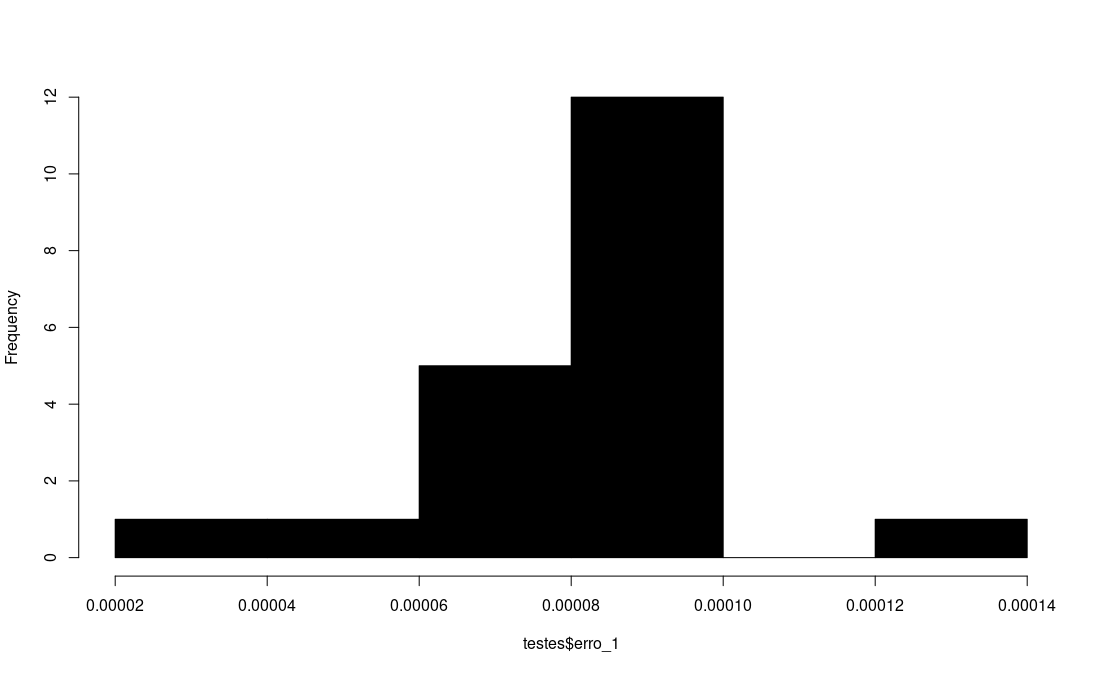
\includegraphics[scale=0.4]{images/histo1.png}
  \label{fig:histo1}
\end{figure}

Seguindo a análise dos testes, foi realizado um teste ANOVA com a amostra de dados coletada. O objetivo foi avaliar a variância dos dados em cada ponto e entre eles, analisando se estes diferem estatisticamente entre si. Com esta análise, obteve-se um $\rho$-valor de 0.6912, com isso tem-se embasamento estatístico para afirmar que os dados no ponto "A" e no ponto "B" são estatisticamente iguais, os erros de pose apresentados nos dois pontos não diferem entre si. Está análise pode ser visualizada na figura \ref*{fig:box1}. 

\begin{figure}[h!]
  \caption{Boxplot do conjunto de dados sem detecção da \textit{tag}.}
  \centering
  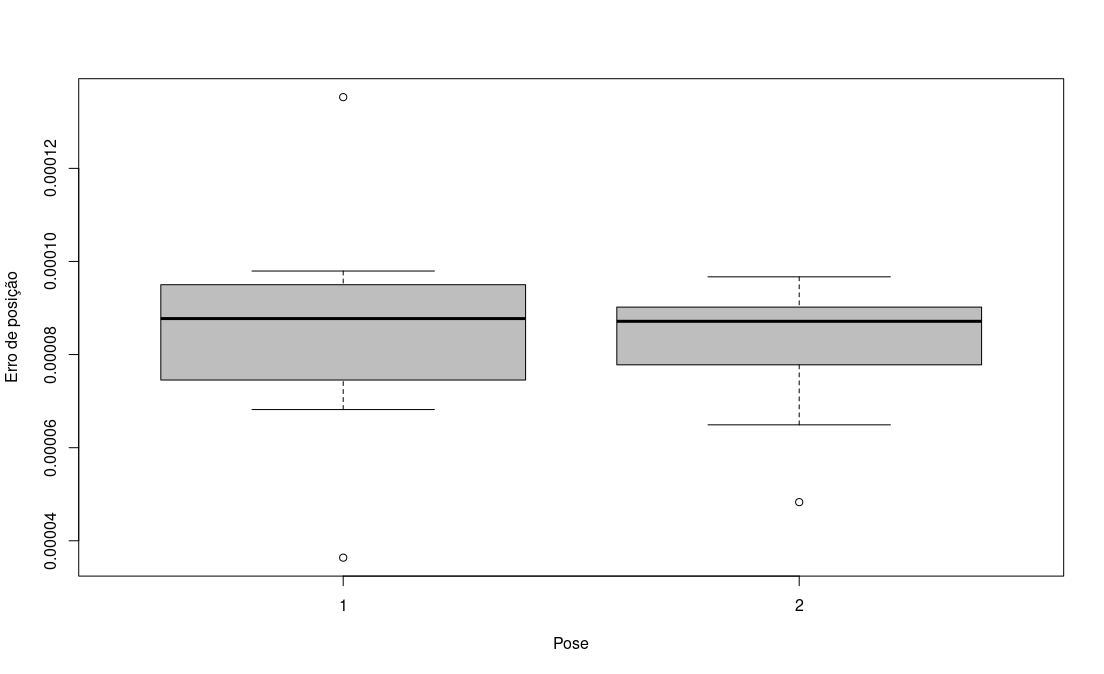
\includegraphics[scale=0.4]{images/box1.png}
  \label{fig:box1}
\end{figure}

Observando a figura \ref*{fig:box1} a pose 1 (A) possui maior variação dos seus dados em relação a pose 2 (B), porém as duas não diferem estatisticamente entre si. 

\subsubsection{Análse de variância com detecção da \textit{tag}}

Foi tomado um novo conjunto de dados, como mostra a tabela \ref*{tab:anova2}. Este experimento foi realizado com variação do operador e posição da caixa. Foram tomados dados de tempo de busca da \textit{tag}, tempo total da missão e o erro de posição do \textit{end-effector}. Também foi observado a porcentagem de sucesso na conclusão da missão, sendo o índice '1' correspondente ao sucesso na missão e o índice '-1' correspondente à falha. 

\begin{table}[H]
  \centering
  \caption{Resultados dos experimentos sem detecção da \textit{tag}.}
  \scalebox{0.8}{%
  \begin{tabular}{r|c|c|c|c|c|c|}
    \cline{2-7}
    \rowcolor[HTML]{EFEFEF} 
    \multicolumn{1}{l|}{\cellcolor[HTML]{EFEFEF}} & \textbf{Operador} & \textbf{Pose} & \textbf{Erro de pose} & \textbf{Tempo de busca} & \textbf{Tempo total} & \textbf{\begin{tabular}[c]{@{}c@{}}Sucesso\\ da missão\end{tabular}} \\ \hline
    \rowcolor[HTML]{FFFFFF} 
    \multicolumn{1}{|r|}{\cellcolor[HTML]{FFFFFF}\textbf{1}} & 1 & A & 0.010451819 & 27.1022 & 93.9316 & 1 \\ \hline
    \rowcolor[HTML]{EFEFEF} 
    \multicolumn{1}{|r|}{\cellcolor[HTML]{EFEFEF}\textbf{2}} & 1 & A & 0.009745817 & 29.1912 & 91.8192 & 1 \\ \hline
    \rowcolor[HTML]{FFFFFF} 
    \multicolumn{1}{|r|}{\cellcolor[HTML]{FFFFFF}\textbf{3}} & 1 & A & 0.010017589 & 27.3904 & 95.6437 & 1 \\ \hline
    \rowcolor[HTML]{EFEFEF} 
    \multicolumn{1}{|r|}{\cellcolor[HTML]{EFEFEF}\textbf{4}} & 1 & A & 0.010819201 & 28.4745 & 90.5214 & 1 \\ \hline
    \rowcolor[HTML]{FFFFFF} 
    \multicolumn{1}{|r|}{\cellcolor[HTML]{FFFFFF}\textbf{5}} & 1 & A & 0.011133634 & 27.7250 & 98.7845 & 1 \\ \hline
    \rowcolor[HTML]{EFEFEF} 
    \multicolumn{1}{|r|}{\cellcolor[HTML]{EFEFEF}\textbf{6}} & 1 & A & 0.010562436 & 28.8388 & 94.6226 & 1 \\ \hline
    \rowcolor[HTML]{FFFFFF} 
    \multicolumn{1}{|r|}{\cellcolor[HTML]{FFFFFF}\textbf{7}} & 1 & A & 0.010132297 & 29.1519 & 101.8420 & 1 \\ \hline
    \rowcolor[HTML]{EFEFEF} 
    \multicolumn{1}{|r|}{\cellcolor[HTML]{EFEFEF}\textbf{8}} & 1 & A & 0.010693537 & 30.2186 & 90.1885 & 1 \\ \hline
    \rowcolor[HTML]{FFFFFF} 
    \multicolumn{1}{|r|}{\cellcolor[HTML]{FFFFFF}\textbf{9}} & 2 & A & 0.010905047 & 30.2317 & 94.0104 & 1 \\ \hline
    \rowcolor[HTML]{EFEFEF} 
    \multicolumn{1}{|r|}{\cellcolor[HTML]{EFEFEF}\textbf{10}} & 2 & A & 0.010469991 & 28.9793 & 96.2312 & 1 \\ \hline
    \rowcolor[HTML]{FFFFFF} 
    \multicolumn{1}{|r|}{\cellcolor[HTML]{FFFFFF}\textbf{11}} & 2 & A & 0.010355747 & 29.0720 & 103.6160 & 1 \\ \hline
    \rowcolor[HTML]{EFEFEF} 
    \multicolumn{1}{|r|}{\cellcolor[HTML]{EFEFEF}\textbf{12}} & 2 & A & 0.010268870 & 28.6952 & 93.0651 & 1 \\ \hline
    \rowcolor[HTML]{FFFFFF} 
    \multicolumn{1}{|r|}{\cellcolor[HTML]{FFFFFF}\textbf{13}} & 2 & A & 0.010230915 & 28.6420 & 87.2120 & 1 \\ \hline
    \rowcolor[HTML]{EFEFEF} 
    \multicolumn{1}{|r|}{\cellcolor[HTML]{EFEFEF}\textbf{14}} & 2 & A & 0.004079350 & 26.8585 & 86.4156 & 1 \\ \hline
    \rowcolor[HTML]{FFFFFF} 
    \multicolumn{1}{|r|}{\cellcolor[HTML]{FFFFFF}\textbf{15}} & 2 & A & 0.004427968 & 26.1808 & 85.7109 & 1 \\ \hline
    \rowcolor[HTML]{EFEFEF} 
    \multicolumn{1}{|r|}{\cellcolor[HTML]{EFEFEF}\textbf{16}} & 2 & A & 0.009985857 & 30.0858 & 90.4296 & 1 \\ \hline
    \rowcolor[HTML]{FFFFFF} 
    \multicolumn{1}{|r|}{\cellcolor[HTML]{FFFFFF}\textbf{17}} & 1 & A & 0.009754491 & 28.2042 & 86.8758 & 1 \\ \hline
    \rowcolor[HTML]{EFEFEF} 
    \multicolumn{1}{|r|}{\cellcolor[HTML]{EFEFEF}\textbf{18}} & 1 & A & 0.010334966 & 28.6983 & 92.2869 & 1 \\ \hline
    \rowcolor[HTML]{FFFFFF} 
    \multicolumn{1}{|r|}{\cellcolor[HTML]{FFFFFF}\textbf{19}} & 1 & A & 0.010058060 & 29.4320 & 94.3545 & 1 \\ \hline
    \rowcolor[HTML]{EFEFEF} 
    \multicolumn{1}{|r|}{\cellcolor[HTML]{EFEFEF}\textbf{20}} & 1 & A & 0.010153228 & 28.1812 & 90.6696 & 1 \\ \hline
    \rowcolor[HTML]{FFFFFF} 
    \multicolumn{1}{|r|}{\cellcolor[HTML]{FFFFFF}\textbf{21}} & 1 & A & 0.010120659 & 29.2442 & 87.1852 & 1 \\ \hline
    \rowcolor[HTML]{EFEFEF} 
    \multicolumn{1}{|r|}{\cellcolor[HTML]{EFEFEF}\textbf{22}} & 1 & A & 0.010105795 & 28.9948 & 88.3569 & 1 \\ \hline
    \rowcolor[HTML]{FFFFFF} 
    \multicolumn{1}{|r|}{\cellcolor[HTML]{FFFFFF}\textbf{23}} & 1 & A & 0.010105795 & 28.9948 & 88.3569 & -1 \\ \hline
    \rowcolor[HTML]{EFEFEF} 
    \multicolumn{1}{|r|}{\cellcolor[HTML]{EFEFEF}\textbf{24}} & 1 & A & 0.011557242 & 32.9496 & 102.3640 & 1 \\ \hline
    \rowcolor[HTML]{FFFFFF} 
    \multicolumn{1}{|r|}{\cellcolor[HTML]{FFFFFF}\textbf{25}} & 2 & A & 0.011245238 & 34.7259 & 98.7636 & 1 \\ \hline
    \rowcolor[HTML]{EFEFEF} 
    \multicolumn{1}{|r|}{\cellcolor[HTML]{EFEFEF}\textbf{26}} & 2 & A & 0.011190817 & 31.1780 & 113.0500 & 1 \\ \hline
    \rowcolor[HTML]{FFFFFF} 
    \multicolumn{1}{|r|}{\cellcolor[HTML]{FFFFFF}\textbf{27}} & 2 & A & 0.010174117 & 28.7923 & 88.9735 & 1 \\ \hline
    \rowcolor[HTML]{EFEFEF} 
    \multicolumn{1}{|r|}{\cellcolor[HTML]{EFEFEF}\textbf{28}} & 2 & A & 0.010007278 & 28.8178 & 91.8702 & 1 \\ \hline
    \rowcolor[HTML]{FFFFFF} 
    \multicolumn{1}{|r|}{\cellcolor[HTML]{FFFFFF}\textbf{29}} & 2 & A & 0.009963924 & 29.0347 & 86.7183 & 1 \\ \hline
    \rowcolor[HTML]{EFEFEF} 
    \multicolumn{1}{|r|}{\cellcolor[HTML]{EFEFEF}\textbf{30}} & 2 & A & 0.010475097 & 28.2422 & 99.1881 & 1 \\ \hline
    \rowcolor[HTML]{FFFFFF} 
    \multicolumn{1}{|r|}{\cellcolor[HTML]{FFFFFF}\textbf{31}} & 2 & A & 0.010741058 & 28.2118 & 91.7459 & 1 \\ \hline
    \rowcolor[HTML]{EFEFEF} 
    \multicolumn{1}{|r|}{\cellcolor[HTML]{EFEFEF}\textbf{32}} & 2 & A & 0.004469904 & 28.4826 & 88.1583 & -1 \\ \hline
    \rowcolor[HTML]{FFFFFF} 
    \multicolumn{1}{|r|}{\cellcolor[HTML]{FFFFFF}\textbf{33}} & 1 & A & 0.010086673 & 28.7112 & 87.9372 & 1 \\ \hline
    \rowcolor[HTML]{EFEFEF} 
    \multicolumn{1}{|r|}{\cellcolor[HTML]{EFEFEF}\textbf{34}} & 1 & A & 0.010515376 & 28.8792 & 92.9002 & 1 \\ \hline
    \rowcolor[HTML]{FFFFFF} 
    \multicolumn{1}{|r|}{\cellcolor[HTML]{FFFFFF}\textbf{35}} & 1 & A & 0.010062717 & 29.1420 & 91.5910 & 1 \\ \hline
    \rowcolor[HTML]{EFEFEF} 
    \multicolumn{1}{|r|}{\cellcolor[HTML]{EFEFEF}\textbf{36}} & 1 & A & 0.010422717 & 29.0783 & 94.3296 & 1 \\ \hline
    \rowcolor[HTML]{FFFFFF} 
    \multicolumn{1}{|r|}{\cellcolor[HTML]{FFFFFF}\textbf{37}} & 1 & A & 0.010185682 & 27.9274 & 88.6971 & 1 \\ \hline
    \rowcolor[HTML]{EFEFEF} 
    \multicolumn{1}{|r|}{\cellcolor[HTML]{EFEFEF}\textbf{38}} & 1 & A & 0.010281946 & 29.7805 & 100.1800 & 1 \\ \hline
    \rowcolor[HTML]{FFFFFF} 
    \multicolumn{1}{|r|}{\cellcolor[HTML]{FFFFFF}\textbf{39}} & 1 & A & 0.013133281 & 20.0540 & 82.3651 & -1 \\ \hline
    \rowcolor[HTML]{EFEFEF} 
    \multicolumn{1}{|r|}{\cellcolor[HTML]{EFEFEF}\textbf{40}} & 1 & A & 0.012344603 & 19.1706 & 81.7740 & 1 \\ \hline

    \end{tabular}}
    \label{tab:anova2}
    % \legend{Fonte: Autoria própria.}
  \end{table}

\begin{table}[H]
    \centering
    \scalebox{0.8}{%
    \begin{tabular}{r|c|c|c|c|c|c|}
      \rowcolor[HTML]{EFEFEF} 
      \multicolumn{1}{l|}{\cellcolor[HTML]{EFEFEF}} & \textbf{Operador} & \textbf{Pose} & \textbf{Erro de pose} & \textbf{Tempo de busca} & \textbf{Tempo total} & \textbf{\begin{tabular}[c]{@{}c@{}}Sucesso\\ da missão\end{tabular}} \\ \hline
      \rowcolor[HTML]{FFFFFF} 
      \multicolumn{1}{|r|}{\cellcolor[HTML]{FFFFFF}\textbf{41}} & 2 & B & 0.005245180 & 20.4070 & 84.7338 & 1 \\ \hline
      \rowcolor[HTML]{EFEFEF} 
      \multicolumn{1}{|r|}{\cellcolor[HTML]{EFEFEF}\textbf{42}} & 2 & B & 0.007158873 & 20.4408 & 84.3043 & 1 \\ \hline
      \rowcolor[HTML]{FFFFFF} 
      \multicolumn{1}{|r|}{\cellcolor[HTML]{FFFFFF}\textbf{43}} & 2 & B & 0.011482759 & 20.7824 & 83.2411 & 1 \\ \hline
      \rowcolor[HTML]{EFEFEF} 
      \multicolumn{1}{|r|}{\cellcolor[HTML]{EFEFEF}\textbf{44}} & 2 & B & 0.087866430 & 23.4152 & 87.9248 & -1 \\ \hline
      \rowcolor[HTML]{FFFFFF} 
      \multicolumn{1}{|r|}{\cellcolor[HTML]{FFFFFF}\textbf{45}} & 2 & B & 0.008514302 & 19.9797 & 86.4344 & 1 \\ \hline
      \rowcolor[HTML]{EFEFEF} 
      \multicolumn{1}{|r|}{\cellcolor[HTML]{EFEFEF}\textbf{46}} & 2 & B & 0.005144988 & 19.8502 & 84.5138 & 1 \\ \hline
      \rowcolor[HTML]{FFFFFF} 
      \multicolumn{1}{|r|}{\cellcolor[HTML]{FFFFFF}\textbf{47}} & 2 & B & 0.013200185 & 19.9392 & 85.7667 & -1 \\ \hline
      \rowcolor[HTML]{EFEFEF} 
      \multicolumn{1}{|r|}{\cellcolor[HTML]{EFEFEF}\textbf{48}} & 2 & B & 0.004874412 & 20.2860 & 80.6176 & 1 \\ \hline
      \rowcolor[HTML]{FFFFFF} 
      \multicolumn{1}{|r|}{\cellcolor[HTML]{FFFFFF}\textbf{49}} & 1 & B & 0.012512453 & 20.7894 & 85.9667 & 1 \\ \hline
      \rowcolor[HTML]{EFEFEF} 
      \multicolumn{1}{|r|}{\cellcolor[HTML]{EFEFEF}\textbf{50}} & 1 & B & 0.014427715 & 19.4977 & 81.7383 & -1 \\ \hline
      \rowcolor[HTML]{FFFFFF} 
      \multicolumn{1}{|r|}{\cellcolor[HTML]{FFFFFF}\textbf{51}} & 1 & B & 0.007453902 & 20.5577 & 82.4847 & 1 \\ \hline
      \rowcolor[HTML]{EFEFEF} 
      \multicolumn{1}{|r|}{\cellcolor[HTML]{EFEFEF}\textbf{52}} & 1 & B & 0.006078841 & 20.4143 & 81.6851 & 1 \\ \hline
      \rowcolor[HTML]{FFFFFF} 
      \multicolumn{1}{|r|}{\cellcolor[HTML]{FFFFFF}\textbf{53}} & 1 & B & 0.009550672 & 19.5227 & 84.7312 & 1 \\ \hline
      \rowcolor[HTML]{EFEFEF} 
      \multicolumn{1}{|r|}{\cellcolor[HTML]{EFEFEF}\textbf{54}} & 1 & B & 0.006123619 & 16.9920 & 74.6466 & 1 \\ \hline
      \rowcolor[HTML]{FFFFFF} 
      \multicolumn{1}{|r|}{\cellcolor[HTML]{FFFFFF}\textbf{55}} & 1 & B & 0.003705978 & 18.6949 & 80.1175 & 1 \\ \hline
      \rowcolor[HTML]{EFEFEF} 
      \multicolumn{1}{|r|}{\cellcolor[HTML]{EFEFEF}\textbf{56}} & 1 & B & 0.006896455 & 19.9972 & 76.2407 & 1 \\ \hline
      \rowcolor[HTML]{FFFFFF} 
      \multicolumn{1}{|r|}{\cellcolor[HTML]{FFFFFF}\textbf{57}} & 2 & B & 0.006869856 & 18.8696 & 79.7714 & 1 \\ \hline
      \rowcolor[HTML]{EFEFEF} 
      \multicolumn{1}{|r|}{\cellcolor[HTML]{EFEFEF}\textbf{58}} & 2 & B & 0.002917472 & 18.4679 & 73.9755 & 1 \\ \hline
      \rowcolor[HTML]{FFFFFF} 
      \multicolumn{1}{|r|}{\cellcolor[HTML]{FFFFFF}\textbf{59}} & 2 & B & 0.004802752 & 19.4849 & 80.2423 & 1 \\ \hline
      \rowcolor[HTML]{EFEFEF} 
      \multicolumn{1}{|r|}{\cellcolor[HTML]{EFEFEF}\textbf{60}} & 2 & B & 0.004557056 & 19.5606 & 77.7174 & 1 \\ \hline
      \rowcolor[HTML]{FFFFFF} 
      \multicolumn{1}{|r|}{\cellcolor[HTML]{FFFFFF}\textbf{61}} & 2 & B & 0.006353444 & 18.5702 & 76.3386 & 1 \\ \hline
      \rowcolor[HTML]{EFEFEF} 
      \multicolumn{1}{|r|}{\cellcolor[HTML]{EFEFEF}\textbf{62}} & 2 & B & 0.007120232 & 19.6487 & 78.9122 & 1 \\ \hline
      \rowcolor[HTML]{FFFFFF} 
      \multicolumn{1}{|r|}{\cellcolor[HTML]{FFFFFF}\textbf{63}} & 2 & B & 0.004832266 & 17.0441 & 77.3120 & 1 \\ \hline
      \rowcolor[HTML]{EFEFEF} 
      \multicolumn{1}{|r|}{\cellcolor[HTML]{EFEFEF}\textbf{64}} & 2 & B & 0.004535360 & 18.0856 & 77.5731 & 1 \\ \hline
      \rowcolor[HTML]{FFFFFF} 
      \multicolumn{1}{|r|}{\cellcolor[HTML]{FFFFFF}\textbf{65}} & 1 & B & 0.007897063 & 17.1585 & 78.1917 & 1 \\ \hline
      \rowcolor[HTML]{EFEFEF} 
      \multicolumn{1}{|r|}{\cellcolor[HTML]{EFEFEF}\textbf{66}} & 1 & B & 0.007330963 & 20.5918 & 81.1574 & 1 \\ \hline
      \rowcolor[HTML]{FFFFFF} 
      \multicolumn{1}{|r|}{\cellcolor[HTML]{FFFFFF}\textbf{67}} & 1 & B & 0.008284862 & 20.2515 & 79.0624 & 1 \\ \hline
      \rowcolor[HTML]{EFEFEF} 
      \multicolumn{1}{|r|}{\cellcolor[HTML]{EFEFEF}\textbf{68}} & 1 & B & 0.008096144 & 19.9652 & 81.4914 & 1 \\ \hline
      \rowcolor[HTML]{FFFFFF} 
      \multicolumn{1}{|r|}{\cellcolor[HTML]{FFFFFF}\textbf{69}} & 1 & B & 0.013425916 & 19.0627 & 79.8650 & -1 \\ \hline
      \rowcolor[HTML]{EFEFEF} 
      \multicolumn{1}{|r|}{\cellcolor[HTML]{EFEFEF}\textbf{70}} & 1 & B & 0.007966466 & 18.6261 & 75.1340 & 1 \\ \hline
      \rowcolor[HTML]{FFFFFF} 
      \multicolumn{1}{|r|}{\cellcolor[HTML]{FFFFFF}\textbf{71}} & 1 & B & 0.008486843 & 18.1093 & 72.8817 & 1 \\ \hline
      \rowcolor[HTML]{EFEFEF} 
      \multicolumn{1}{|r|}{\cellcolor[HTML]{EFEFEF}\textbf{72}} & 1 & B & 0.007759457 & 18.7750 & 77.1361 & 1 \\ \hline
      \rowcolor[HTML]{FFFFFF} 
      \multicolumn{1}{|r|}{\cellcolor[HTML]{FFFFFF}\textbf{73}} & 2 & B & 0.012489658 & 20.1018 & 77.2422 & 1 \\ \hline
      \rowcolor[HTML]{EFEFEF} 
      \multicolumn{1}{|r|}{\cellcolor[HTML]{EFEFEF}\textbf{74}} & 2 & B & 0.008122309 & 18.6224 & 77.0045 & 1 \\ \hline
      \rowcolor[HTML]{FFFFFF} 
      \multicolumn{1}{|r|}{\cellcolor[HTML]{FFFFFF}\textbf{75}} & 2 & B & 0.012097601 & 20.3431 & 79.8706 & 1 \\ \hline
      \rowcolor[HTML]{EFEFEF} 
      \multicolumn{1}{|r|}{\cellcolor[HTML]{EFEFEF}\textbf{76}} & 2 & B & 0.087776215 & 17.5113 & 77.7186 & 1 \\ \hline
      \rowcolor[HTML]{FFFFFF} 
      \multicolumn{1}{|r|}{\cellcolor[HTML]{FFFFFF}\textbf{77}} & 2 & B & 0.006999748 & 17.3791 & 74.1548 & 1 \\ \hline
      \rowcolor[HTML]{EFEFEF} 
      \multicolumn{1}{|r|}{\cellcolor[HTML]{EFEFEF}\textbf{78}} & 2 & B & 0.008223493 & 18.3666 & 76.5340 & 1 \\ \hline
      \rowcolor[HTML]{FFFFFF} 
      \multicolumn{1}{|r|}{\cellcolor[HTML]{FFFFFF}\textbf{79}} & 2 & B & 0.008721295 & 19.4229 & 73.9818 & 1 \\ \hline
      \rowcolor[HTML]{EFEFEF} 
      \multicolumn{1}{|r|}{\cellcolor[HTML]{EFEFEF}\textbf{80}} & 2 & B & 0.008375202 & 18.6691 & 73.7671 & 1 \\ \hline
    \end{tabular}}
    \legend{Fonte: Autoria própria.}
\end{table}

Observando a tabela \ref*{tab:anova2}, os testes apresentaram 91.25\% de sucesso, ou seja, dos 80 testes realizados, em 73 obteve-se sucesso no pressionamento do botão. A tabela \ref*{tab:resumo1} resume alguns indicadores importantes das três saídas do sistema (tempo de busca, tempo total da missão e erro de pose).

\begin{table}[h!]
  \centering
  \caption{Resumo dos conjuntos de dados das variáveis de saída.}
  \scalebox{0.9}{%
  \begin{tabular}{c|c|c|c|}
    \cline{2-4}
    \rowcolor[HTML]{EFEFEF} 
    \multicolumn{1}{l|}{\cellcolor[HTML]{FFFFFF}} & \textbf{Média} & \textbf{\begin{tabular}[c]{@{}c@{}}Desvio \\ padrão\end{tabular}} & \textbf{\begin{tabular}[c]{@{}c@{}}$\rho$-valor\\ (Shapiro-Wilk)\end{tabular}} \\ \hline
    \rowcolor[HTML]{FFFFFF} 
    \multicolumn{1}{|c|}{\cellcolor[HTML]{FFFFFF}\textbf{Tempo de busca}} & 23.95025 & 5.035711 & 1.103e-07 \\ \hline
    \rowcolor[HTML]{EFEFEF} 
    \multicolumn{1}{|c|}{\cellcolor[HTML]{EFEFEF}\textbf{Tempo total}} & 86.06149 & 8.343288 & 0.02409 \\ \hline
    \rowcolor[HTML]{FFFFFF} 
    \multicolumn{1}{|c|}{\cellcolor[HTML]{FFFFFF}\textbf{Erro de pose}} & 0.01095061 & 0.0126478 & 2.2e-16 \\ \hline
    \end{tabular}}
    \label{tab:resumo1}
    \legend{Fonte: Autoria própria.}
  \end{table}

Os testes de normalidade apresentaram valores de $\rho$-valor inferiores a 0.05, ou seja, a hipótese nula não pode ser rejeitada, logo os dados seguem uma distribuição normal. 


\begin{table}[H]
  \centering
  \caption{Tabela dos valores de $\rho$-valor do teste ANOVA. }
  \scalebox{1}{%
  \begin{tabular}{c|c|}
    \cline{2-2}
     & \cellcolor[HTML]{EFEFEF}\textbf{p-valor} \\ \hline
    \rowcolor[HTML]{FFFFFF} 
    \multicolumn{1}{|c|}{\cellcolor[HTML]{FFFFFF}\textbf{Erro de pose}} & 0.525 \\ \hline
    \rowcolor[HTML]{EFEFEF} 
    \multicolumn{1}{|c|}{\cellcolor[HTML]{EFEFEF}\textbf{Tempo de busca}} & 2.2e-16 \\ \hline
    \rowcolor[HTML]{FFFFFF} 
    \multicolumn{1}{|c|}{\cellcolor[HTML]{FFFFFF}\textbf{Tempo total}} & 2.2e-16 \\ \hline
    \end{tabular}}
    \label{tab:resumo2}
    \legend{Fonte: Autoria própria.}
  \end{table}


Realizando o teste do ANOVA, podemos visualizar a variância dos pontos A e B em relação ao erro de pose, tempo de busca e tempo total da missão. A tabela \ref*{tab:resumo2} apresenta o $\rho$-valor para cada conjunto de dados, e a partir dessa análise podemos chegar a conclusão que a hipótese nula não pode ser rejeitada para o erro de pose assim como visto na análise passada, ou seja, os dados obtidos do erro de posição do \textit{end-effector} nos pontos A e B são estatisticamente iguais. Já os dados dos tempo de busca e tempo total da missão apresentam $\rho$-valor menor que 0.05, logo a hipótese nula é rejeitada e pode-se concluir que os dados diferem entre si, como mostram os \textit{boxplots} das figuras \ref*{fig:box4} e \ref*{fig:box5}.

\begin{figure}[H]
  \caption{\textit{Boxplot} da variância do tempo de busca entre os pontos A e B. }
  \centering
  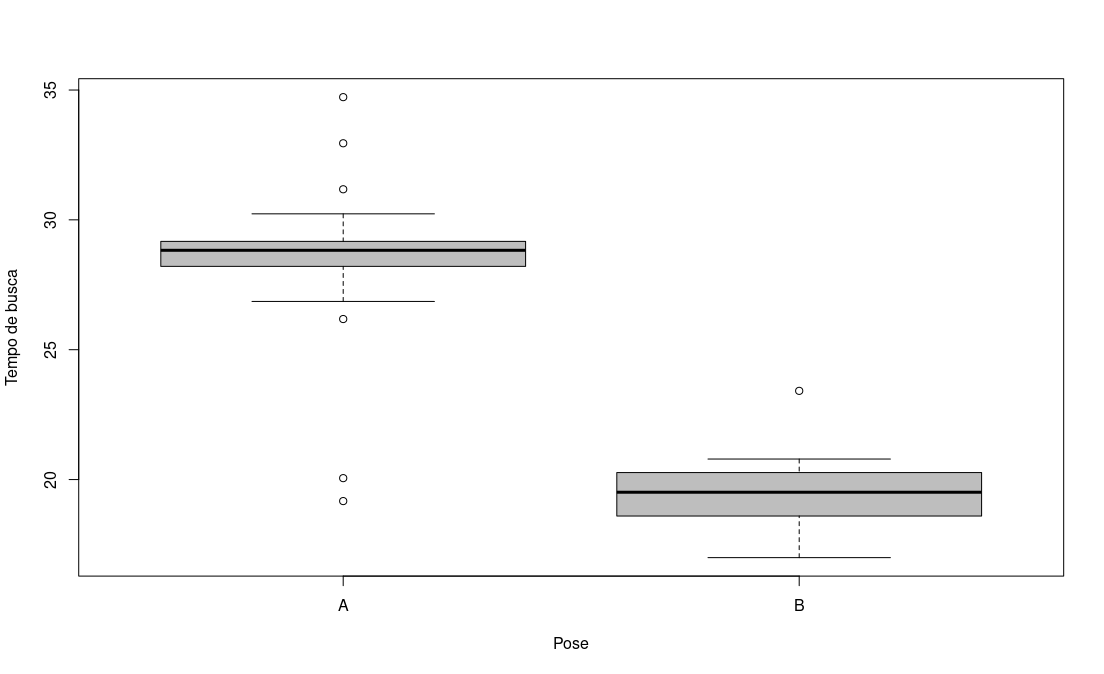
\includegraphics[scale=0.45]{images/box4_tb.png}
  \label{fig:box4}
  \legend{Fonte: Autoria própria.}
\end{figure}
\begin{figure}[H]
  \caption{\textit{Boxplot} da variância do tempo total da missão entre os pontos A e B. }
  \centering
  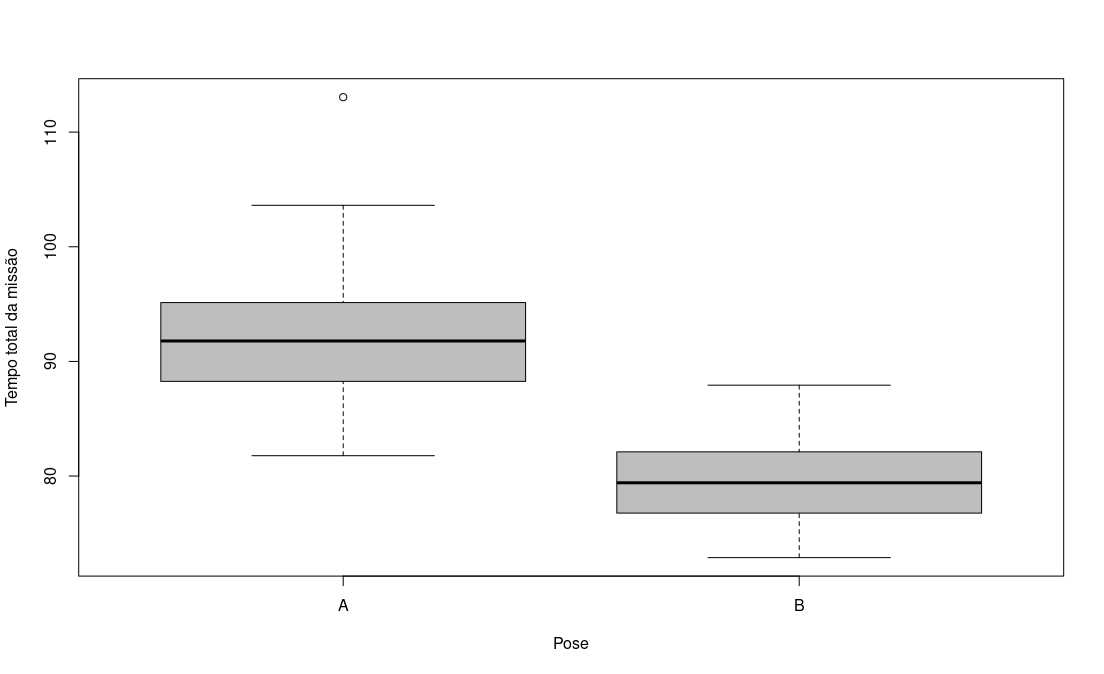
\includegraphics[scale=0.45]{images/box3_tt.png}
  \label{fig:box5}
  \legend{Fonte: Autoria própria.}
\end{figure}

% As figuras xx, yy e zz apresentadas a seguir apresentam o histograma de cada uma das variáveis e de forma visual pode-se notar a distribuição dos dados. 

% \begin{figure}[H]
%   \caption{Histograma dos erros de pose no ponto A. }
%   \centering
%   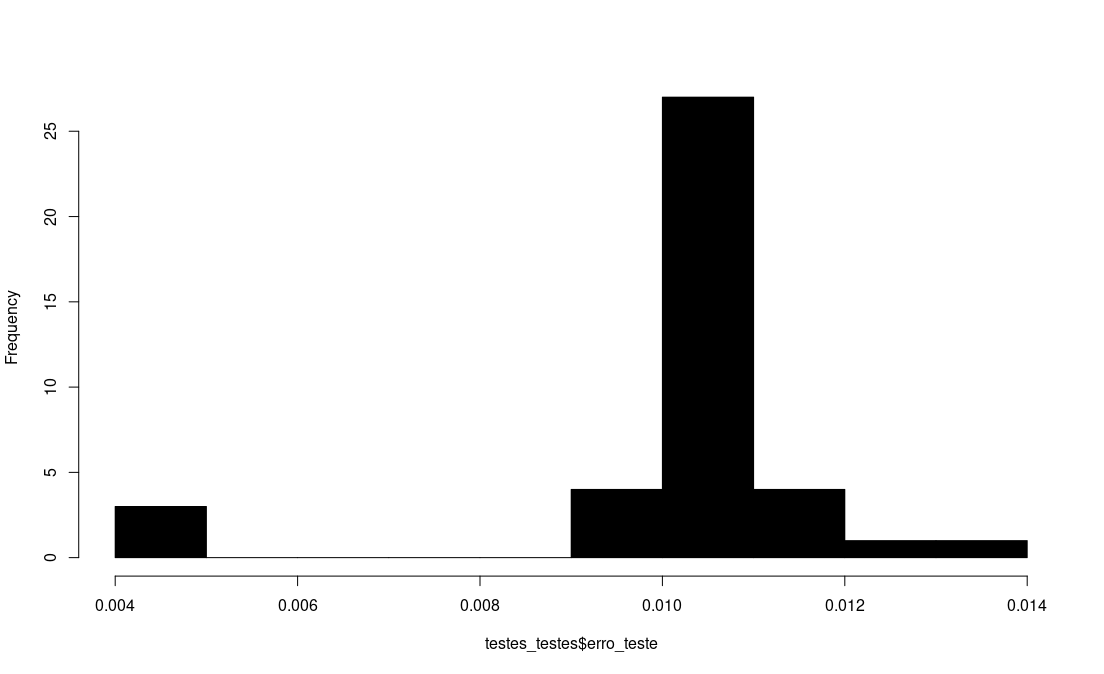
\includegraphics[scale=0.35]{images/histo2_ea.png}
%   \label{fig:histo2}
% \end{figure}
% \begin{figure}[H]
%   \caption{Histograma dos erros de pose no ponto B.}
%   \centering
%   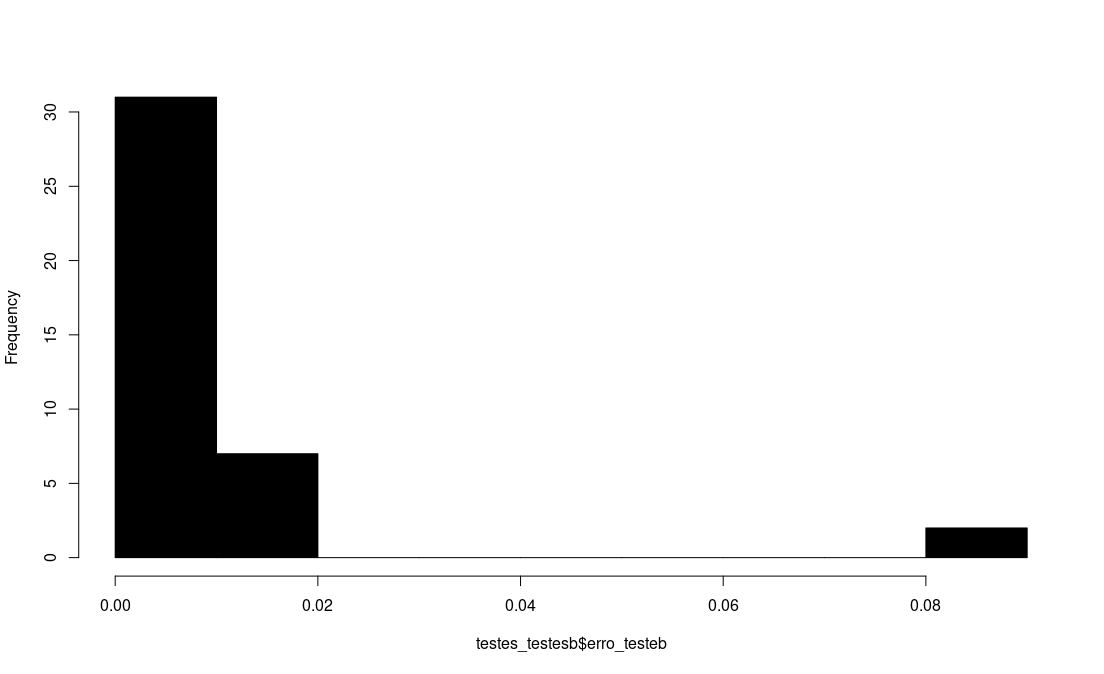
\includegraphics[scale=0.35]{images/histo3_eb.png}
%   \label{fig:histo3}
% \end{figure}
% \begin{figure}[H]
%   \caption{Histograma do tempo de busca no ponto A.}
%   \centering
%   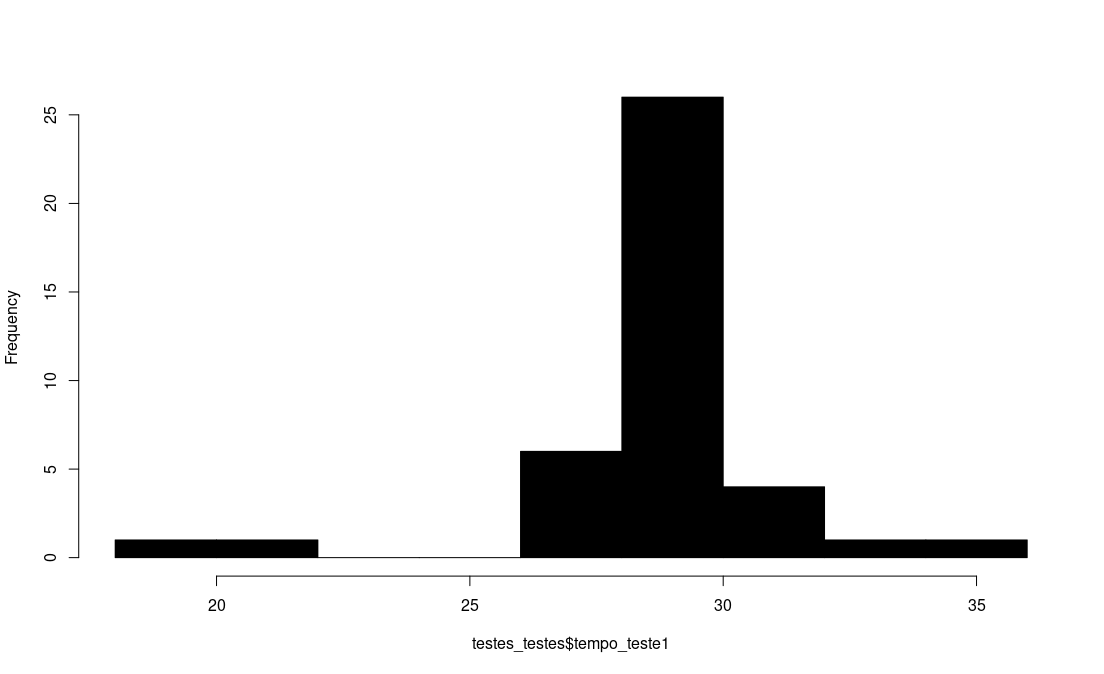
\includegraphics[scale=0.35]{images/histo_tba.png}
%   \label{fig:histo4}
% \end{figure}
% \begin{figure}[H]
%   \caption{Histograma do tempo de busca no ponto B.}
%   \centering
%   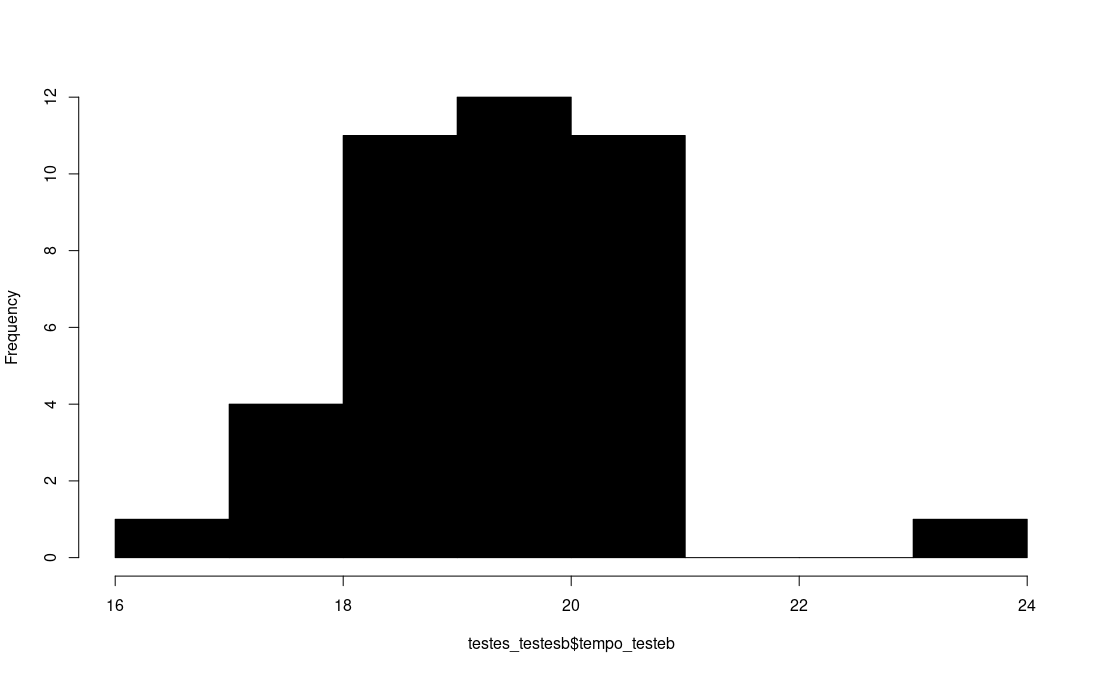
\includegraphics[scale=0.35]{images/histo_tbb.png}
%   \label{fig:histo5}
% \end{figure}
% \begin{figure}[H]
%   \caption{Histograma do tempo total da missão no ponto A.}
%   \centering
%   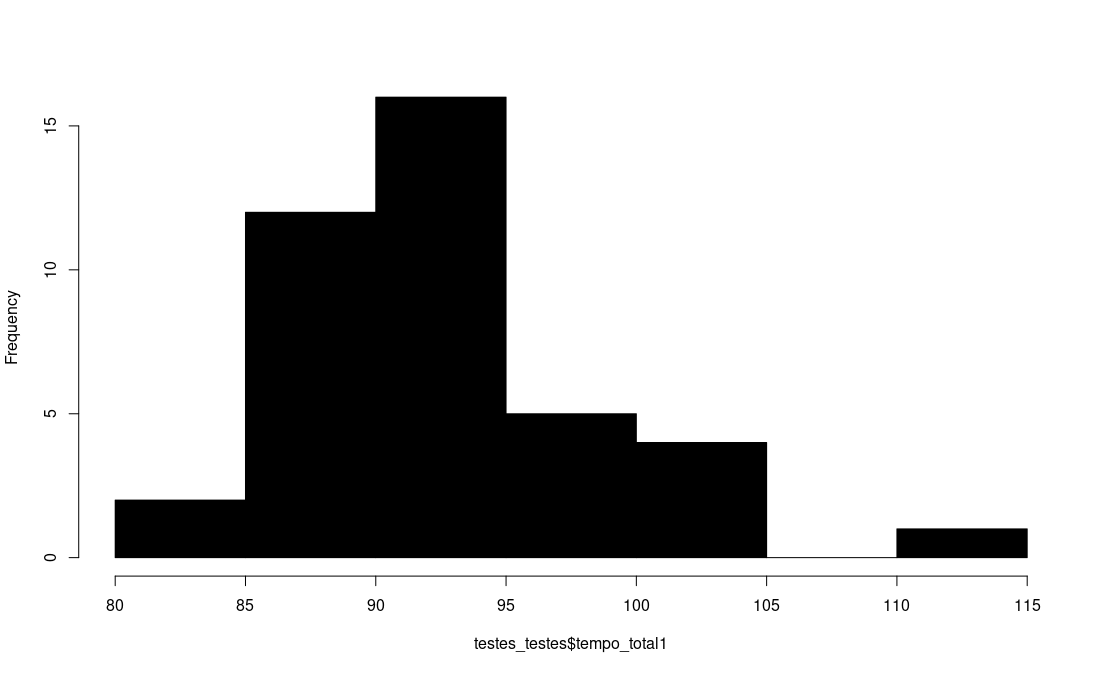
\includegraphics[scale=0.35]{images/histo_tta.png}
%   \label{fig:histo6}
% \end{figure}
% \begin{figure}[H]
%   \caption{Histograma do tempo total da missão no ponto B.}
%   \centering
%   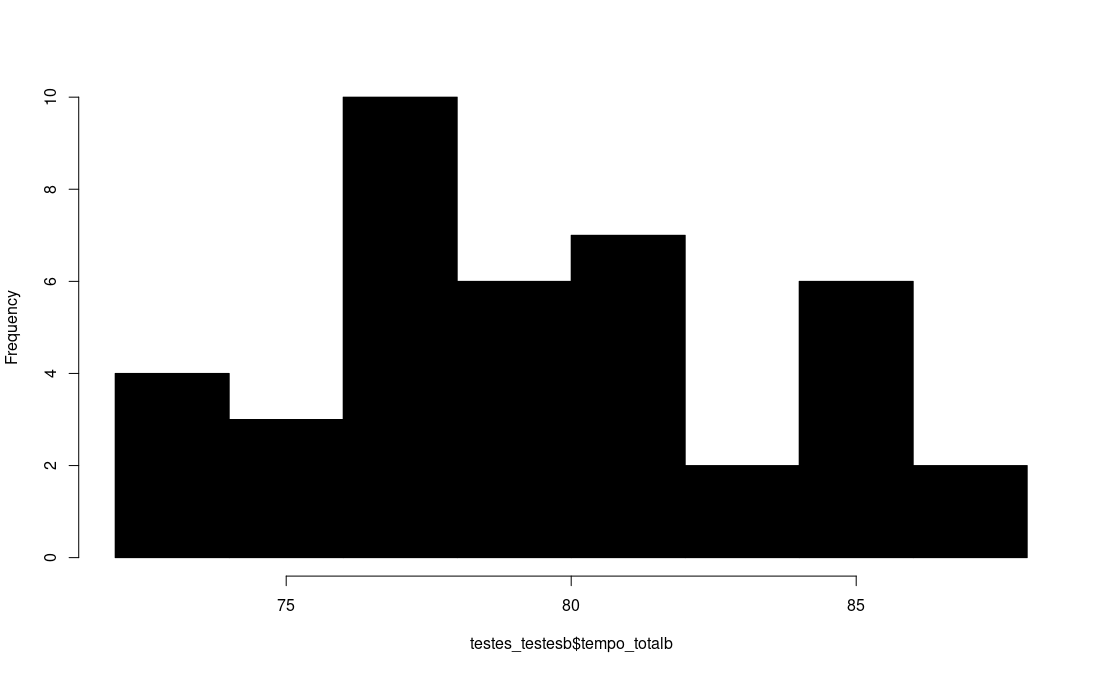
\includegraphics[scale=0.35]{images/histo_ttb.png}
%   \label{fig:histo7}
% \end{figure}


\subsection{Análise de repetibilidade e reprodutibilidade}

Como forma de avaliação do sistema robótico, também foi adotado um estudo de repetibilidade e reprodutibilidade do sistema. Com isso, foram adotados os dados da tabela \ref*{tab:anova2}. Foram tomadas 20 medições de cada operador para cada pose da caixa, totalizando 80 testes e assim foram obtidos os seguintes dados apresentados na figura \ref*{fig:rr1} e \ref*{fig:rr2}.


\begin{figure}[h!]
  \caption{Modelo completo teste R\&R para tempo de busca.}
  \centering
  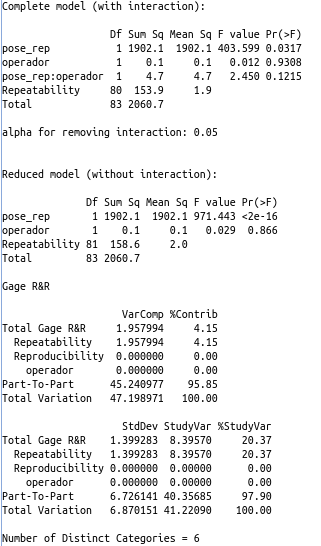
\includegraphics[scale=0.55]{images/rr_tb.png}
  \label{fig:rr1}
  \legend{Fonte: Autoria própria.}
\end{figure}

% \begin{figure}[H]
%   \caption{Modelo completo teste R\&R para tempo total da missão.}
%   \centering
%   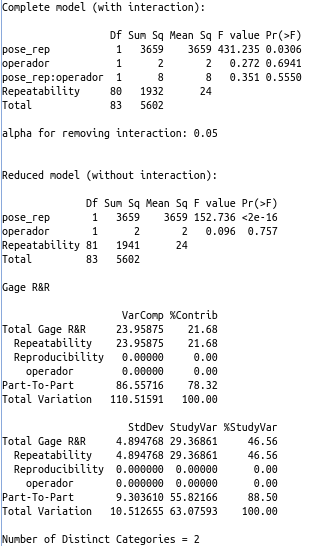
\includegraphics[scale=0.6]{images/rr_tt.png}
%   \label{fig:rr2}
%   \legend{Fonte: Autoria própria.}
% \end{figure}

Observando a figura \ref*{fig:rr1}, correspondente ao teste de R\&R para o tempo busca do marcador visual, neste teste percebe-se o número de categorias igual a 6, número considerável e acima de valores de referências, o que demonstra que o sistema de medição pode ser utilizado para análise dos dados. Outro ponto importante para observado é o indicador "\textit{Total Gage R\&R}", que foi calculado em 20.37, inferior a 30\% (Valor máximo aceitável adotado em algumas literaturas). 

O sistema sendo aceitável para análise, pode-se observar outros indicadores importantes para análise, como exemplo do $\rho$-valor, que mostra a maior influência na variação devido a pose da caixa, não ocorrendo influência do operador ou da interação entre operador e pose. O indicador "\textit{Part-to-Part}" indica que aproximadamento 98\% da variação do sistema deve-se a própria variação de pose da caixa, o que demonstra que o sistema possui repetibilidade e reprodutibilidade, quanto a variável de tempo de busca.

\begin{figure}[H]
  \caption{Modelo completo teste R\&R para tempo total da missão.}
  \centering
  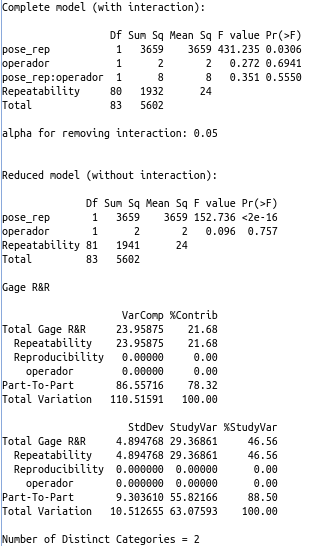
\includegraphics[scale=0.55]{images/rr_tt.png}
  \label{fig:rr2}
  \legend{Fonte: Autoria própria.}
\end{figure}

O mesmo não pode ser observado na figura \ref*{fig:rr2}, onde o número de categorias apresentados é baixo e o índice "\textit{Total Gage R\&R}" foi calculado em 46.56\%, acima do valor máximo de referência (30\%), o que mostra que o sistema de medição não é aceitável quando observado a variável de tempo total da missão.  

Seguindo a análise dos dados obtidos no estudo de repetibilidade e reprodutibilidade do sistema para o tempo de busca, visualizamos cartas na figura \ref*{fig:rr3} que possibilita um melhor entendimento do sistema de medição.

\begin{figure}[H]
  \caption{Gráficos do estudo R\&R para tempo de busca.}
  \centering
  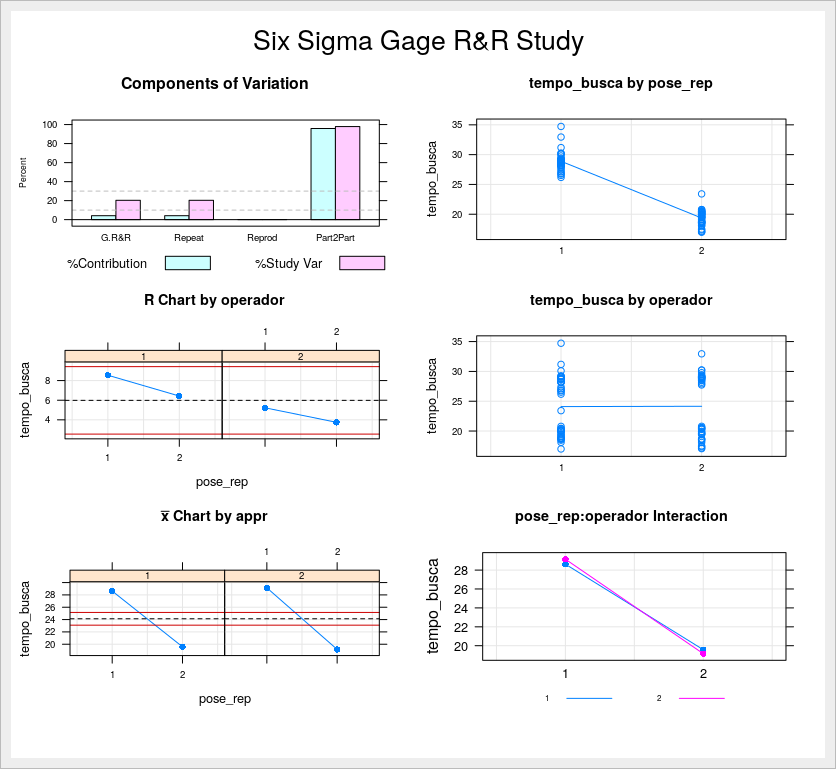
\includegraphics[scale=0.7]{images/rr_bus.png}
  \label{fig:rr3}
  \legend{Fonte: Autoria própria.}
\end{figure}

A carta "Componentes de variação" representa atribuições da variação do sistema, e como observado na figura \ref*{fig:rr3}, a variação deve-se principalmente a "peça por peça" ou "parte por parte", o que é desejável, demonstrando que o sistema de medição é aceitável para análise do tempo de busca do manipulador. 

A carta R é uma carta de controle de amplitudes que representa graficamente a consistência do operador. Os pontos apresentados na figura \ref*{fig:rr3} estão dentro dos limites máximos e mínimos, ou seja, é sinal de que os operadores estão realizando os testes de forma consistente.

Os pontos apresentados na carta Xbar, na figura \ref*{fig:rr3}, os dados estão acima ou abaixo dos limites de controle. Estes resultados indicam que a variação
entre as poses são maiores que a variação do dispositivo de medição. 

Outro ponto importante de ser destacado é o gráfico de interação entre o operador e o tempo de busca (figura \ref*{fig:rr3}), a barra horizontal visualizada, demonstra que os operadores estão realizando medições semelhantes entre si, com variações semelhantes entre as medidas máximas e mínimas do tempo de busca. 



% \begin{knitrout}
%   \begin{kframe}
%   \begin{verbatim}
%       Complete model (with interaction):

%       Df Sum Sq Mean Sq F value Pr(>F)
%   pose_rep           1   3659    3659 431.235 0.0306
%   operador           1      2       2   0.272 0.6941
%   pose_rep:operador  1      8       8   0.351 0.5550
%   Repeatability     80   1932      24               
%   Total             83   5602                       

%   alpha for removing interaction: 0.05 


%   Reduced model (without interaction):

%   Df Sum Sq Mean Sq F value Pr(>F)
%   pose_rep       1   3659    3659 152.736 <2e-16
%   operador       1      2       2   0.096  0.757
%   Repeatability 81   1941      24               
%   Total         83   5602                       

%   Gage R&R

%         VarComp %Contrib
%   Total Gage R&R     23.95875    21.68
%   Repeatability    23.95875    21.68
%   Reproducibility   0.00000     0.00
%   operador        0.00000     0.00
%   Part-To-Part       86.55716    78.32
%   Total Variation   110.51591   100.00

%         StdDev StudyVar %StudyVar
%   Total Gage R&R     4.894768 29.36861     46.56
%   Repeatability    4.894768 29.36861     46.56
%   Reproducibility  0.000000  0.00000      0.00
%   operador       0.000000  0.00000      0.00
%   Part-To-Part       9.303610 55.82166     88.50
%   Total Variation   10.512655 63.07593    100.00

%   Number of Distinct Categories = 2 
% \end{verbatim}
% \end{kframe}
% \end{knitrout}


% \begin{knitrout}
%   \begin{kframe}
%   \begin{verbatim}
%   Complete model (with interaction):

%   Df Sum Sq Mean Sq F value Pr(>F)
% pose_rep           1 1902.1  1902.1 403.599 0.0317
% operador           1    0.1     0.1   0.012 0.9308
% pose_rep:operador  1    4.7     4.7   2.450 0.1215
% Repeatability     80  153.9     1.9               
% Total             83 2060.7                       

% alpha for removing interaction: 0.05 


% Reduced model (without interaction):

% Df Sum Sq Mean Sq F value Pr(>F)
% pose_rep       1 1902.1  1902.1 971.443 <2e-16
% operador       1    0.1     0.1   0.029  0.866
% Repeatability 81  158.6     2.0               
% Total         83 2060.7                       

% Gage R&R

%     VarComp %Contrib
% Total Gage R&R     1.957994     4.15
% Repeatability    1.957994     4.15
% Reproducibility  0.000000     0.00
% operador       0.000000     0.00
% Part-To-Part      45.240977    95.85
% Total Variation   47.198971   100.00

%     StdDev StudyVar %StudyVar
% Total Gage R&R    1.399283  8.39570     20.37
% Repeatability   1.399283  8.39570     20.37
% Reproducibility 0.000000  0.00000      0.00
% operador      0.000000  0.00000      0.00
% Part-To-Part      6.726141 40.35685     97.90
% Total Variation   6.870151 41.22090    100.00

% Number of Distinct Categories = 6 
% \end{verbatim}
% \end{kframe}
% \end{knitrout}


\section{Conclusões dos testes estatísticos}

Após estudo dos dados obtidos a partir de testes no manipulador robótico, verifica-se que os dados apresentaram distribuição normal, o que possibilita uma análise confiável dos mesmos, comprovando isso através de histogramas apresentados durante a seção. 

Também é possível observar nos testes realizados que o algoritmo de planejamento de trajetória RRT CONNECT apresentou melhor resultado em relação ao Kpiece, bem como a velocidade pouco influenciou nos testes, mostrando que a melhor configuração para o sistema para as missões impostas é utilizando o algoritmo RRT. 

Não houve diferença no erro de posicionamento do \textit{end-effector} quando observado as poses A e B e com ou sem detecção do marcador visual, ou seja, pode-se concluir que o manipulador robótico apresenta erro constante nas poses analisadas. É observado também que o tempo de busca e tempo total da missão diferem entre as poses. 

Por fim, conclui-se que a análise de repetibilidade e reprodutibilidade foi positiva quando observados os dados da variável tempo de busca do marcador visual, uma vez que o sistema de medição atendeu ao teste; enquanto que para a variável tempo total da missão os resultados não foram de todo satisfatórios, indicando possíveis direções de melhoria no sistema. 

%------------------------------------------------------------------
%\section{Análise dos experimentos}
%\label{sec:doe}


%------------------------------------------------------------------
%\section{Avaliação da prontidão tecnológica}
%\label{sec:trl}


	\chapter{CONFIABILIDADE DO SISTEMA}
\label{chap:conf}
A fim de verificar-se a confiabilidade do sistema, foi realizado o levantamento de cada componente que constitui o manipulador robótico e o estudo detalhado das prováveis falhas. Para isso, foi utilizado o \textit{\acs{FMECA}} com o propósito de analisar cada sub-sistema, como pode ser visto nas tabelas da seção \ref{sec:fmeca}. 

Na seção \ref{sec:fta} foi desenvolvida a análise da árvore de falhas do sistema, método que permite através de um processo lógico dedutivo chegar-se às causas básicas de um problema de proporções maiores.

%------------------------------------------------------------------
\section{Análise dos modos e efeitos de falhas}
\label{sec:fmeca}
  Nas Tabelas \ref{tab:sistema_potencia}, \ref{tab:sistema_aquisicao}, \ref{tab:sistema_estrutural}, \ref{tab:sistema_atuacao} e \ref{tab:sistema_processamento}  estão representadas informações referentes ao estudo sistemático e estrutura das falhas potenciais para os sub-sistemas de potência, de aquisição, estrutural, de atuação e de processamento, respectivamente. 



  \begin{table}[H]
    \caption{ \textit{FMECA} do sub-sistema de potência}
    \begin{adjustbox}{max width=\textwidth}
    \begin{tabular}{|c|c|c|c|c|c|c|c|c|}
    \hline
    \rowcolor[HTML]{EFEFEF} 
    \multicolumn{9}{|c|}{\cellcolor[HTML]{EFEFEF}\textbf{Análise do Tipo e Efeito de Falha}} \\ \hline
    \multicolumn{9}{|c|}{\textbf{Sub-sistema de potência}} \\ \hline
    \rowcolor[HTML]{EFEFEF} 
    \textbf{Função(ões)} &
      \textbf{\begin{tabular}[c]{@{}c@{}}Modo(s) de falha\\ em potencial\end{tabular}} &
      \textbf{\begin{tabular}[c]{@{}c@{}}Efeito(s) potencial(is)\\ da falha\end{tabular}} &
      \textbf{S} &
      \textbf{\begin{tabular}[c]{@{}c@{}}Causa(s)\\ potenciais\end{tabular}} &
      \textbf{O} &
      \textbf{D} &
      \textbf{C} &
      \textbf{\begin{tabular}[c]{@{}c@{}}Ação(ões) \\ recomendada(s)\end{tabular}} \\ \hline
     &
       &
      \begin{tabular}[c]{@{}c@{}}Comprometimento dos\\  dados transmitidos\end{tabular} &
      6 &
      Fissura dos fios &
      3 &
      5 &
      90 &
       \\ \cline{3-8}
    \multirow{-2}{*}{\begin{tabular}[c]{@{}c@{}}Transmissão \\ de dados\end{tabular}} &
      \multirow{-2}{*}{\begin{tabular}[c]{@{}c@{}}Incapacidade de \\ transmissão\\de dados\end{tabular}} &
      \begin{tabular}[c]{@{}c@{}}Perda da capacidade \\ de transmissão \\ de dados\end{tabular} &
      8 &
      \begin{tabular}[c]{@{}c@{}}Desgaste causado \\ pelo tempo\end{tabular} &
      2 &
      1 &
      16 &
      \multirow{-2}{*}{\begin{tabular}[c]{@{}c@{}}Manutenções \\ preventivas\end{tabular}} \\ \hline
     &
       &
      \begin{tabular}[c]{@{}c@{}}Perda da capacidade\\de transmissão de energia\end{tabular} &
      8 &
      \begin{tabular}[c]{@{}c@{}}Derretimento por \\ temperatura elevada\end{tabular} &
      1 &
      1 &
      8 &
      \begin{tabular}[c]{@{}c@{}}Manutenções \\ preventivas\end{tabular} \\ \cline{3-9} 
    \multirow{-2}{*}{\begin{tabular}[c]{@{}c@{}}Transmissão \\ de energia\end{tabular}} &
      \multirow{-2}{*}{\begin{tabular}[c]{@{}c@{}}Incapacidade de\\transmissão de energia\end{tabular}} &
      \begin{tabular}[c]{@{}c@{}}Má qualidade da \\ energia transmitida\end{tabular} &
      6 &
      Torção dos fios &
      3 &
      5 &
      90 &
      \multicolumn{1}{l|}{} \\ \hline
     &
       &
       &
       &
      \begin{tabular}[c]{@{}c@{}}Má conexão \\ com fonte de tensão\end{tabular} &
      3 &
      6 &
      162 &
      \begin{tabular}[c]{@{}c@{}}Verificar conexão\\  com fonte\end{tabular} \\ \cline{5-9} 
    \multirow{-2}{*}{\begin{tabular}[c]{@{}c@{}}Alimentação\\ do sistema\end{tabular}} &
      \multirow{-2}{*}{\begin{tabular}[c]{@{}c@{}}Incapacidade \\ em fornecer energia\end{tabular}} &
      \multirow{-2}{*}{\begin{tabular}[c]{@{}c@{}}Não energização\\  do sistema\end{tabular}} &
      \multirow{-2}{*}{9} &
      \begin{tabular}[c]{@{}c@{}}Desgaste nas soldas \\ causado pelo tempo\end{tabular} &
      4 &
      7 &
      252 &
      \begin{tabular}[c]{@{}c@{}}Verificar continuidade\\ na placa do circuito\end{tabular} \\ \hline
    \end{tabular}
    \end{adjustbox}
    \legend{Fonte: Autoria própria.}
    \label{tab:sistema_potencia}
    \end{table}



\begin{table}[H]
  \caption{ \textit{FMECA} do sub-sistema aquisição}
  \begin{adjustbox}{max width=\textwidth}
  \begin{tabular}{|c|c|c|c|c|c|c|c|c|}
  \hline
  \rowcolor[HTML]{EFEFEF}
  \multicolumn{9}{|c|}{\cellcolor[HTML]{EFEFEF}\textbf{Análise do Tipo e Efeito de Falha}} \\ \hline
  \rowcolor[HTML]{FFFFFF} 
  \multicolumn{9}{|c|}{\cellcolor[HTML]{FFFFFF}\textbf{Sub-sistema de aquisição}} \\ \hline
  \rowcolor[HTML]{EFEFEF} 
  \textbf{Função(ões)} & \textbf{\begin{tabular}[c]{@{}c@{}}Modo(s) de falha \\ em potencial\end{tabular}} & \textbf{\begin{tabular}[c]{@{}c@{}}Efeito(s) potencial(is) \\ da falha\end{tabular}} & \textbf{S} & \textbf{\begin{tabular}[c]{@{}c@{}}Causa(s) \\ potenciais\end{tabular}} & \textbf{O} & \textbf{D} & \textbf{C} & \textbf{\begin{tabular}[c]{@{}c@{}}Ação(ões) \\ recomendada(s)\end{tabular}} \\ \hline
  \rowcolor[HTML]{FFFFFF} 
  \cellcolor[HTML]{FFFFFF} & \begin{tabular}[c]{@{}c@{}}Incapacidade de \\ obter dados visuais\end{tabular} & \cellcolor[HTML]{FFFFFF} & \cellcolor[HTML]{FFFFFF} & \begin{tabular}[c]{@{}c@{}}Obstrução do campo \\ de visão da câmera\end{tabular} & 2 & 1 & 16 & \cellcolor[HTML]{FFFFFF} \\ \cline{2-2} \cline{5-8}
  \rowcolor[HTML]{FFFFFF} 
  \cellcolor[HTML]{FFFFFF} & \cellcolor[HTML]{FFFFFF} & \cellcolor[HTML]{FFFFFF} & \cellcolor[HTML]{FFFFFF} & \begin{tabular}[c]{@{}c@{}}Baixa visibilidade \\ do ambiente\end{tabular} & 2 & 5 & 80 & \cellcolor[HTML]{FFFFFF} \\ \cline{5-8}
  \rowcolor[HTML]{FFFFFF} 
  \cellcolor[HTML]{FFFFFF} & \multirow{-2}{*}{\cellcolor[HTML]{FFFFFF}\begin{tabular}[c]{@{}c@{}}Ruptura da estrutura \\ de fixação da câmera\end{tabular}} & \multirow{-3}{*}{\cellcolor[HTML]{FFFFFF}\begin{tabular}[c]{@{}c@{}}Perda da capacidade \\ de obter dados visuais\end{tabular}} & \multirow{-3}{*}{\cellcolor[HTML]{FFFFFF}8} & \begin{tabular}[c]{@{}c@{}}Calibração incorreta \\ da câmera\end{tabular} & 3 & 1 & 24 & \multirow{-3}{*}{\cellcolor[HTML]{FFFFFF}\begin{tabular}[c]{@{}c@{}}Verificar condições do\\ ambiente antes das missões\end{tabular}} \\ \cline{2-9} 
  \rowcolor[HTML]{FFFFFF} 
  \cellcolor[HTML]{FFFFFF} & \cellcolor[HTML]{FFFFFF} & \cellcolor[HTML]{FFFFFF} & \cellcolor[HTML]{FFFFFF} & Set-up incorreto & 2 & 7 & 84 & \cellcolor[HTML]{FFFFFF} \\ \cline{5-8}
  \rowcolor[HTML]{FFFFFF} 
  \multirow{-5}{*}{\cellcolor[HTML]{FFFFFF}\begin{tabular}[c]{@{}c@{}}Aquisição de \\ dados visuais\end{tabular}} & \multirow{-2}{*}{\cellcolor[HTML]{FFFFFF}\begin{tabular}[c]{@{}c@{}}Coleta de dados \\ inconsistentes ou insuficientes\end{tabular}} & \multirow{-2}{*}{\cellcolor[HTML]{FFFFFF}\begin{tabular}[c]{@{}c@{}}Comprometimento \\ dos dados\end{tabular}} & \multirow{-2}{*}{\cellcolor[HTML]{FFFFFF}6} & \begin{tabular}[c]{@{}c@{}}Falha no canal \\ de comunicação\end{tabular} & 4 & 7 & 168 & \multirow{-2}{*}{\cellcolor[HTML]{FFFFFF}\begin{tabular}[c]{@{}c@{}}Verificar cabeamento\\ do sistema\end{tabular}} \\ \hline
  \end{tabular}
\end{adjustbox}
\legend{Fonte: Autoria própria.}
\label{tab:sistema_aquisicao}
  \end{table}

      \begin{table}[H]
      \caption{ \textit{FMECA} do sub-sistema estrutural}
      \begin{adjustbox}{max width=\textwidth}
        \begin{tabular}{|c|c|c|l|c|l|l|c|c|}
        \hline
        \rowcolor[HTML]{EFEFEF} 
        \multicolumn{9}{|c|}{\cellcolor[HTML]{EFEFEF}\textbf{Análise do Tipo e Efeito de Falha}} \\ \hline
        \multicolumn{9}{|c|}{\textbf{Sub-sistema estrutural}} \\ \hline
        \rowcolor[HTML]{EFEFEF} 
        \textbf{Função(ões)} &
          \textbf{\begin{tabular}[c]{@{}c@{}}Modo(s) de falha\\ em potencial\end{tabular}} &
          \textbf{\begin{tabular}[c]{@{}c@{}}Efeito(s) potencial(is)\\ da falha\end{tabular}} &
          \textbf{S} &
          \textbf{\begin{tabular}[c]{@{}c@{}}Causa(s)\\ potenciais\end{tabular}} &
          \textbf{O} &
          \textbf{D} &
          \textbf{C} &
          \textbf{\begin{tabular}[c]{@{}c@{}}Ação(ões)\\ \\ recomendada(s)\end{tabular}} \\ \hline
         &
           &
           &
           &
          \begin{tabular}[c]{@{}c@{}}Excesso de \\ peso aplicado\end{tabular} &
          2 &
          1 &
          16 &
           \\ \cline{5-8}
         &
           &
          \multirow{-2}{*}{Ruptura do conector} &
          \multirow{-2}{*}{8} &
          \begin{tabular}[c]{@{}c@{}}Desgaste \\ pelo tempo\end{tabular} &
          2 &
          5 &
          80 &
          \multirow{-2}{*}{\begin{tabular}[c]{@{}c@{}}Verificar a\\ fabricação da peça\end{tabular}} \\ \cline{3-9} 
         &
           &
           &
           &
          \begin{tabular}[c]{@{}c@{}}Set-up \\ incorreto\end{tabular} &
          4 &
          6 &
          144 &
           \\ \cline{5-8}
        \multirow{-4}{*}{\begin{tabular}[c]{@{}c@{}}Ligar o frame \\ ao perfil de \\ alumínio\end{tabular}} &
          \multirow{-4}{*}{\begin{tabular}[c]{@{}c@{}}Incapacidade de\\  sustentar o perfil\end{tabular}} &
          \multirow{-2}{*}{Trinca do conector} &
          \multirow{-2}{*}{6} &
          \begin{tabular}[c]{@{}c@{}}Defeito de \\ fabricação\end{tabular} &
          5 &
          6 &
          180 &
          \multirow{-2}{*}{\begin{tabular}[c]{@{}c@{}}Verificar as \\ condições de peso aplicadas\end{tabular}} \\ \hline
         &
          \begin{tabular}[c]{@{}c@{}}Danificação \\ estrutural\end{tabular} &
          Ruptura do perfil &
          8 &
          Sobrecarga &
          2 &
          4 &
          64 &
          \begin{tabular}[c]{@{}c@{}}Cuidado no \\ manuseamento \\ dos perfis\end{tabular} \\ \cline{2-9} 
        \multirow{-2}{*}{\begin{tabular}[c]{@{}c@{}}Compor\\ estrutura mecânica\end{tabular}} &
          \begin{tabular}[c]{@{}c@{}}Folga entre \\ conexões\end{tabular} &
          Empeno do perfil &
          6 &
          Colisão &
          4 &
          2 &
          48 &
          \begin{tabular}[c]{@{}c@{}}Definir \\ área de trabalho\end{tabular} \\ \hline
        \end{tabular}
        \end{adjustbox}
        \legend{Fonte: Autoria própria.}
        \label{tab:sistema_estrutural}
        \end{table}



        \begin{table}[H]
          \caption{ \textit{FMECA} do sub-sistema de atuação}
          \begin{adjustbox}{max width=\textwidth}
           \begin{tabular}{|c|c|c|c|c|c|c|c|c|}
              \hline
              \rowcolor[HTML]{EFEFEF} 
              \multicolumn{9}{|c|}{\cellcolor[HTML]{EFEFEF}\textbf{Análise do Tipo e Efeito de Falha}} \\ \hline
              \multicolumn{9}{|c|}{\textbf{Sub-sistema de atuação}} \\ \hline
              \rowcolor[HTML]{EFEFEF} 
              \textbf{Função(ões)} &
                \textbf{\begin{tabular}[c]{@{}c@{}}Modo(s) de falha\\ em potencial\end{tabular}} &
                \textbf{\begin{tabular}[c]{@{}c@{}}Efeito(s) potencial(is)\\ da falha\end{tabular}} &
                \textbf{S} &
                \textbf{\begin{tabular}[c]{@{}c@{}}Causa(s)\\ potenciais\end{tabular}} &
                \textbf{O} &
                \textbf{D} &
                \textbf{C} &
                \textbf{\begin{tabular}[c]{@{}c@{}}Ação(ões)\\ recomendada(s)\end{tabular}} \\ \hline
              \begin{tabular}[c]{@{}c@{}}Movimentação \\ do manipulador\end{tabular} &
                \begin{tabular}[c]{@{}c@{}}Rotação inconsistente \\ com o desejado\end{tabular} &
                \begin{tabular}[c]{@{}c@{}}Perda de desempenho \\ (velocidade; controle)\end{tabular} &
                6 &
                \begin{tabular}[c]{@{}c@{}}Emperramento \\ parcial\end{tabular} &
                4 &
                6 &
                144 &
                \begin{tabular}[c]{@{}c@{}}Inspeções \\ periódicas\end{tabular} \\ \hline
               &
                Curto circuito &
                Parada do motor &
                8 &
                \begin{tabular}[c]{@{}c@{}}Cabeamento \\ incorreto\end{tabular} &
                2 &
                5 &
                80 &
                 \\ \cline{2-8}
               &
                Perda de comunicação &
                 &
                 &
                 &
                 &
                 &
                 &
                 \\ \cline{2-2}
              \multirow{-3}{*}{\begin{tabular}[c]{@{}c@{}}Fornecer o torque\\  mínimo de sustentação\end{tabular}} &
                Tensão insuficiente &
                \multirow{-2}{*}{Perda de desempenho} &
                \multirow{-2}{*}{6} &
                \multirow{-2}{*}{\begin{tabular}[c]{@{}c@{}}Falha na \\ alimentação\end{tabular}} &
                \multirow{-2}{*}{4} &
                \multirow{-2}{*}{5} &
                \multirow{-2}{*}{120} &
                \multirow{-3}{*}{\begin{tabular}[c]{@{}c@{}}Medir corrente\\  nos terminais\end{tabular}} \\ \hline
              \end{tabular}
              \end{adjustbox}
              \legend{Fonte: Autoria própria.}
              \label{tab:sistema_atuacao}
              \end{table}


              \begin{table}[H]
                \caption{ \textit{FMECA} do sub-sistema de processamento}
                \begin{adjustbox}{max width=\textwidth}
                \begin{tabular}{|c|c|c|c|c|c|c|c|c|}
                \hline
                \rowcolor[HTML]{EFEFEF} 
                \multicolumn{9}{|c|}{\cellcolor[HTML]{EFEFEF}\textbf{Análise do Tipo e Efeito de Falha}} \\ \hline
                \multicolumn{9}{|c|}{\textbf{Sub-sistema de processamento}} \\ \hline
                \rowcolor[HTML]{EFEFEF} 
                \textbf{Função(ões)} &
                  \textbf{\begin{tabular}[c]{@{}c@{}}Modo(s) de falha\\ em potencial\end{tabular}} &
                  \textbf{\begin{tabular}[c]{@{}c@{}}Efeito(s) potencial(is)\\ da falha\end{tabular}} &
                  \textbf{S} &
                  \textbf{\begin{tabular}[c]{@{}c@{}}Causa(s)\\ potenciais\end{tabular}} &
                  \textbf{O} &
                  \textbf{D} &
                  \textbf{C} &
                  \textbf{\begin{tabular}[c]{@{}c@{}}Ação(ões) \\ recomendada(s)\end{tabular}} \\ \hline
                 &
                   &
                   &
                   &
                  \begin{tabular}[c]{@{}c@{}}Queima/ danificação \\ de componentes\end{tabular} &
                  3 &
                  8 &
                  216 &
                  \begin{tabular}[c]{@{}c@{}}Manutenção \\ preditiva\end{tabular} \\ \cline{5-9} 
                 &
                   &
                   &
                   &
                  \begin{tabular}[c]{@{}c@{}}Falha no sistema\\ operacional\end{tabular} &
                  2 &
                  8 &
                  144 &
                  \begin{tabular}[c]{@{}c@{}}Executar teste de \\ verificação do software\end{tabular} \\ \cline{5-9} 
                 &
                   &
                   &
                   &
                  \begin{tabular}[c]{@{}c@{}}Falha na porta de \\ comunicação\end{tabular} &
                  2 &
                  2 &
                  36 &
                  \begin{tabular}[c]{@{}c@{}}Exectutar teste de entrada\\ e saída de dados com \textit{NUC}\end{tabular} \\ \cline{5-9} 
                \multirow{-4}{*}{\begin{tabular}[c]{@{}c@{}}Processamento dos\\ dados\end{tabular}} &
                  \multirow{-4}{*}{\begin{tabular}[c]{@{}c@{}}Não processamento dos \\ dados do sistema principal\end{tabular}} &
                  \multirow{-4}{*}{Não funcionamento} &
                  \multirow{-4}{*}{9} &
                  \begin{tabular}[c]{@{}c@{}}Problemas de contato\\ elétrico\end{tabular} &
                  2 &
                  3 &
                  54 &
                  \begin{tabular}[c]{@{}c@{}}Inspeções periódicas\\ em bancada\end{tabular} \\ \hline
                \end{tabular}
                \end{adjustbox}
                \legend{Fonte: Autoria própria.}
                \label{tab:sistema_processamento}
                \end{table}
          

%------------------------------------------------------------------
%\section{Diagrama de blocos da Confiabilidade}
%\label{sec:diag}

%------------------------------------------------------------------
\section{Análise da árvore de falhas}
\label{sec:fta}

Na Figura \ref{fig:arvore_falha} encontra-se a árvore de falhas do sistema do manipulador JeRoTIMON. Observa-se que caso o manipulador não consiga realizar a tarefa de pressionar o botão, duas causas principais devem ser investigadas: a conexão entre as TF's, realizada a partir do pacote \textit{Bir Marker Localization}, ou o planejamento de trajetória, realizado pelo \textit{Moveit}. Para a primeira causa, devem ser verificadas as configurações do pacote e da câmera, bem como a orientação dos componentes envolvidos no processo de detecção. Já para solucionar os problemas correspondentes ao planejamento de trajetória, deve-se observar se a pose desejada está dentro do \textit{workspace} do manipulador e se o \textit{plugin} de cinemática inversa utilizado está sendo capaz de realizar as conversões necessárias para a pose desejada. 

\begin{figure}[H]
  \centering
  \caption{Árvore de falhas do sistema.}
  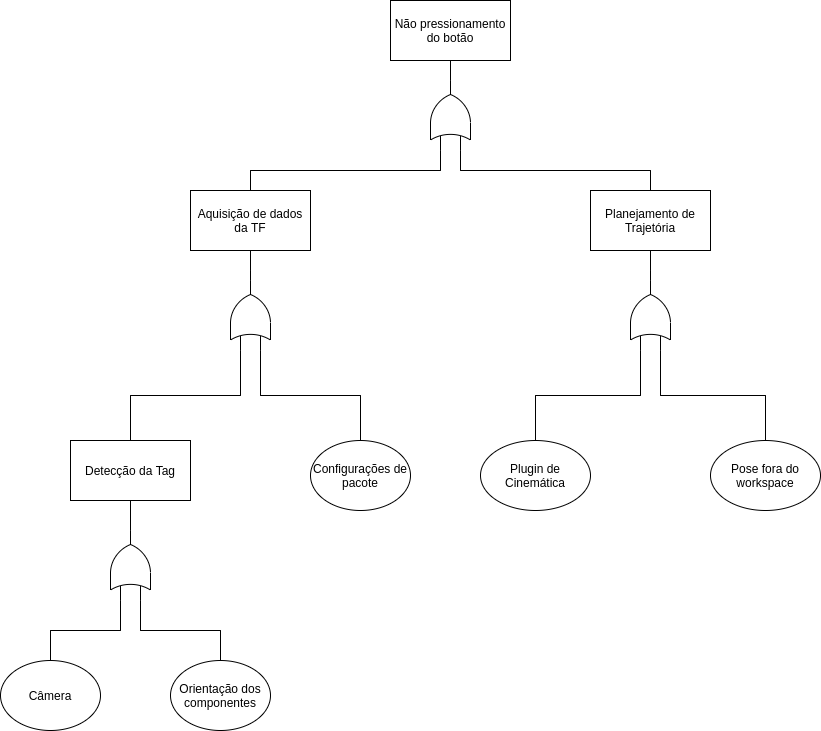
\includegraphics[scale=0.5]{images/arvore_falhas.png}
  \legend{Fonte: Autoria própria.}
  \label{fig:arvore_falha}
\end{figure}

	\chapter{GESTÃO DO CONHECIMENTO}
\label{chap:conhec}

Neste capítulo estão descritas as lições aprendidas durante o processo de desenvolvimento do protótipo que foram criadas a partir da comparação entre o que era esperado e o que realmente aconteceu em cada etapa do projeto. Esta sub-seção engloba desde a fase inicial do planejamento até a construção do modelo real.

Além das lições aprendidas, as seções \ref{sec:guia_simulacao} e \ref{sec:guia_real} trazem os guias de uso para a simulação e o modelo real, respectivamente, com o propósito de auxiliar o usuário na replicação dos experimentos realizados neste relatório.

%------------------------------------------------------------------
\section{Lições aprendidas}
\label{sec:licap}

A Tabela \ref{tab:licoes_aprendidas}  mostra como foi estruturada cada lição aprendida abordando os seguintes aspectos: Tema, Fase, Impacto, O que ocorreu?, Como resolveu?, Resultados e Recomendações para os próximos projetos. O objetivo deste estudo é a correção dos impactos negativos para os projetos subsequentes.


\begin{table}[H]
  \caption{Lições aprendidas}
  \begin{adjustbox}{max width=\textwidth}
  \begin{tabular}{|c|c|c|c|c|c|c|}
  \hline
  \rowcolor[HTML]{EFEFEF} 
  \multicolumn{7}{|c|}{\cellcolor[HTML]{EFEFEF}\textbf{LIÇÕES APRENDIDAS}} \\ \hline
  \rowcolor[HTML]{FFFFFF} 
  \textbf{Tema} & \textbf{Fase} & \textbf{Impacto} & \textbf{O que ocorreu?} & \textbf{Como resolveu?} & \textbf{Resultados} & \textbf{\begin{tabular}[c]{@{}c@{}}Recomendações para\\ os próximos projetos\end{tabular}} \\ \hline
  \rowcolor[HTML]{EFEFEF} 
  Gestão & Planejamento & Negativo & \begin{tabular}[c]{@{}c@{}}Ausência de uma \\ metodologia\\ de trabalho\end{tabular} & \begin{tabular}[c]{@{}c@{}}Reunião com foco em definir\\ metodologia de projeto\end{tabular} & \begin{tabular}[c]{@{}c@{}}Evolução na \\ comunicação dos \\ membros\end{tabular} & \begin{tabular}[c]{@{}c@{}}Antes de começar o projeto\\ realizar reunião para definição\\ de metodologia\end{tabular} \\ \hline
  \rowcolor[HTML]{FFFFFF} 
  Gestão & Planejamento & Negativo & \begin{tabular}[c]{@{}c@{}}Ausência de uma ferramenta\\ para gestão de projeto\end{tabular} & \begin{tabular}[c]{@{}c@{}}Escolha de uma ferramenta\\ gratuita e de fácil aplicação\end{tabular} & \begin{tabular}[c]{@{}c@{}}Melhoria na\\ organização\\ das atividades\end{tabular} & \begin{tabular}[c]{@{}c@{}}Definição prévia de uma\\ ferramenta de gestão de \\ projeto\end{tabular} \\ \hline
  \rowcolor[HTML]{EFEFEF} 
  Gestão & Execução & Negativo & \begin{tabular}[c]{@{}c@{}}Montagens e desmontagens\\ do manipulador\end{tabular} & \begin{tabular}[c]{@{}c@{}}Planejamento\\ prévio das atividades\end{tabular} & \begin{tabular}[c]{@{}c@{}}Otimização do \\ tempo\end{tabular} & \begin{tabular}[c]{@{}c@{}}Cronograma definido \\ as atividades a serem \\ realizadas\end{tabular} \\ \hline
  \rowcolor[HTML]{FFFFFF} 
  Tecnológico & Execução & Negativo & \begin{tabular}[c]{@{}c@{}}Falha no \\ dimensionamento\\ das peças\end{tabular} & \begin{tabular}[c]{@{}c@{}}Consultoria sobre\\ materiais aplicados\\ na confecção\end{tabular} & \begin{tabular}[c]{@{}c@{}}Obtenção de peças\\ com maior resistência\\ mecânica\end{tabular} & \begin{tabular}[c]{@{}c@{}}Pesquisa e consultoria prévia\\ antes da modelagem das \\ peças\end{tabular} \\ \hline
  \rowcolor[HTML]{EFEFEF} 
  Tecnológico & Execução & Negativo & \begin{tabular}[c]{@{}c@{}}Dificuldade em planejamento\\ de trajetória para \\ determinadas poses do robô\end{tabular} & \begin{tabular}[c]{@{}c@{}}Utilização do plugin\\ Track-IK\end{tabular} & \begin{tabular}[c]{@{}c@{}}Maior eficiência\\ de planejamento\end{tabular} & \begin{tabular}[c]{@{}c@{}}Pesquisa e consultoria prévia\\ do pacote mais adequado\\ para o projeto\end{tabular} \\ \hline
  \rowcolor[HTML]{FFFFFF} 
  Tecnológico & Execução & Negativo & \begin{tabular}[c]{@{}c@{}}Motor dynamixel \\ (H54-200-S500-R PRO)\\ parou de funcionar\end{tabular} & \begin{tabular}[c]{@{}c@{}}Realizado a Análise 8D \\ para fazer investigação do\\ ocorrido\end{tabular} & \begin{tabular}[c]{@{}c@{}}Compreensão de \\ que há procedimentos a serem feitos \\ antes de utilizar um produto\end{tabular} & \begin{tabular}[c]{@{}c@{}}Realizar leitura meticulosa \\ do manual do produto \\ para saber quais são os \\ procedimentos\end{tabular} \\ \hline
  \end{tabular}
  \end{adjustbox}
  \legend{Fonte: Autoria própria.}
  \label{tab:licoes_aprendidas}
\end{table}




%------------------------------------------------------------------
\section{Guia de uso para simulação}
\label{sec:guia_simulacao}

Para replicar a simulação do manipulador robótico Timon-HM é necessário seguir os passos descritos nesta seção. Recomenda-se a utilização do Ubuntu 18.04 LTS e o \textit{\acs{ROS}} Melodic Morenia.

Antes de inserir o pacote do manipulador no \textit{workspace} é fundamental que sejam instalados os pacotes requeridos para este. Primeiramente, no terminal, segue-se os comandos listados:

\begin{itemize}
  \item Instalar MoveIt:
  \begin{lstlisting}[frame=single]
    $ sudo apt-get install ros-melodic-moveit
  \end{lstlisting}
  \item Instalar pacote de ferramentas visuais do MoveIt:
  \begin{lstlisting}[frame=single]
    $ sudo apt-get install ros-melodic-moveit-visual-tools
  \end{lstlisting}
  \item Instalar TRAC-IK para resolução da cinemática:
  \begin{lstlisting}[frame=single]
    $ sudo apt-get install ros-melodic-trac-ik-kinematics-
    plugin
  \end{lstlisting}
  \item Instalar pacote de controle no \textit{Gazebo} \textit{\acs{ROS}}:
  \begin{lstlisting}[frame=single]
    $ sudo apt-get install ros-melodic-gazebo-ros-control
  \end{lstlisting}
  \item Instalar pacote do controlador do \textit{\acs{ROS}}:
  \begin{lstlisting}[frame=single]
    $ sudo apt-get install ros-melodic-controller-*
  \end{lstlisting}
  \item Instalar pacote controlador de posição do \textit{\acs{ROS}}:
  \begin{lstlisting}[frame=single]
    $ sudo apt-get install ros-melodic-position-controller
  \end{lstlisting}
  \item Instalar pacote controlador de esforço do \textit{\acs{ROS}}:
  \begin{lstlisting}[frame=single]
    $ sudo apt-get install ros-melodic-effort-controller
  \end{lstlisting}
  \item Instalar pacote de juntas do \textit{\acs{ROS}}:
  \begin{lstlisting}[frame=single]
    $ sudo apt install ros-melodic-joint-*
  \end{lstlisting}
  \item Instalar pacote de controle do \textit{\acs{ROS}}:
  \begin{lstlisting}[frame=single]
    $ sudo apt install ros-melodic-ros-control
  \end{lstlisting}
\end{itemize}


Antes de instalar o pacote \textit{bir\_marker\_localization} é necessária a instalação do \textit{\acs{OpenCV}} versão 3.3.1, este possui o guia de instalação próprio disponível em:

\url{https://www.learnopencv.com/install-opencv3-on-ubuntu/}.

Após a instalação do \textit{\acs{OpenCV}}, para clonar o repositório do \textit{bir\_marker\_localization} segue-as as seguintes etapas, no terminal:

\begin{itemize}
  \item Criar um \textit{workspace} para adicionar dentro deste os pacotes que serão usados na simulação.
  \begin{lstlisting}[frame=single]
    $ mkdir nomedoworkspace_ws
  \end{lstlisting}
  \item Entrar no \textit{workspace}:
  \begin{lstlisting}[frame=single]
    $ cd nomedoworkspace_ws
  \end{lstlisting}
  \item Criar a pasta \textit{source}\footnote{Pasta onde contém os arquivos fonte.}:
  \begin{lstlisting}[frame=single]
    $ mkdir src
  \end{lstlisting}
  \item Entrar no \textit{source}:
  \begin{lstlisting}[frame=single]
    $ cd src
  \end{lstlisting}
  \item Clonar o repositório \textit{Bir Marker Localization} para \textit{workspace} (Verificar qual a \textit{branch} estável):
  \begin{lstlisting}[frame=single]
    $ git clone https://github.com/Brazilian-Institute-of-
    Robotics/bir_marker_localization.git
  \end{lstlisting}
  
  \item Clonar o pacote do manipulador para dentro da pasta src:
  \begin{lstlisting}[frame=single]
    $ git clone -b feature/simulation https://github.com/Brazilian-Institute-of-
    Robotics/timon_hm_manipulator.git
  \end{lstlisting}

  \item Clonar o pacote do \textit{Open Manipulator} para dentro da pasta src:
  \begin{lstlisting}[frame=single]
    $ git clone https://github.com/ROBOTIS-GIT/open_
    manipulator_msgs.git
  \end{lstlisting}

  \item Retornar para a raiz do \textit{workspace}:
  \begin{lstlisting}[frame=single]
    $ cd ..
  \end{lstlisting}
 
  \item Compilar o \textit{workspace}:
  \begin{lstlisting}[frame=single]
    $ catkin_make
  \end{lstlisting}
  \item Ativar o ambiente virtual do \textit{workspace}:
  \begin{lstlisting}[frame=single]
    $ source devel/setup.bash
  \end{lstlisting}
\end{itemize}

Após realizar os procedimentos citados o \textit{workspace} estará configurado para executar a simulação, com os seguintes comandos (cada comando terá que ser inserido em uma aba do terminal):

\begin{itemize}
  \item Iniciar a simulação no \textit{Gazebo}:
  \begin{lstlisting}[frame=single]
    $ roslaunch manipulator_gazebo gazebo.launch
  \end{lstlisting}
  \item Iniciar pacote MoveIt do Timon-HM:
  \begin{lstlisting}[frame=single]
    $ roslaunch manipulator_gazebo moveit_demo.launch
  \end{lstlisting}
  \item Iniciar o bir\_marker\_localization:
  \begin{lstlisting}[frame=single]
   $ roslaunch timon_demo bir_marker_localization.launch
  \end{lstlisting}
  \item Iniciar o algoritmo de busca do marcador visual e para acionar o painel elétrico:
  \begin{lstlisting}[frame=single]
    $ roslaunch timon_demo push_button_simulation.launch
  \end{lstlisting}  
\end{itemize}




%------------------------------------------------------------------
\section{Guia de uso para o modelo real}
\label{sec:guia_real}

Para replicar o modelo real do manipulador a versão do Ubuntu, do \textit{\acs{ROS}} e os pacotes necessários são os mesmos descritos na seção \ref{sec:guia_simulacao}. Após a instalação dos pacotes, a seguir estão descritas as etapas subsequentes:

\begin{itemize}
  % \item Instalar os pacotes:
  % \begin{lstlisting}[frame=single]
  %   $ sudo apt install ros-melodic-ros-control 
  %   ros-melodic-gazebo-ros-control 
  %   ros-melodic-controller-manager 
  %   ros-melodic-joint-trajectory-controller 
  %   ros-melodic-joint-state-controller 
  %   ros-melodic-position-controllers 
  %   ros-melodic-trac-ik-kinematics-plugin
  % \end{lstlisting}
  \item Criar \textit{workspace} e a pasta \textit{source}:
  \begin{lstlisting}[frame=single]
    $ mkdir -p catkin_ws/src
  \end{lstlisting} 
  \item Entrar no \textit{workspace} e no \textit{source}:
  \begin{lstlisting}[frame=single]
    $ cd  catkin_ws/src
  \end{lstlisting} 
  \item Clonar para dentro da pasta \textit{source} o repositório do manipulador:
  \begin{lstlisting}[frame=single]
    $ git clone https://github.com/Brazilian-Institute-of-
    Robotics/timon_hm_manipulator.git 
  \end{lstlisting}
  \item Clonar para dentro do \textit{source} o repositório do \textit{Bir Marker Localization}:
  \begin{lstlisting}[frame=single]
    $ git clone -b final_settings https://github.com/
    Brazilian-Institute-of-Robotics/
    bir_marker_localization.git
  \end{lstlisting}  
  \item Clonar para dentro do \textit{source} o repositório do \textit{Open Manipulator}:
  \begin{lstlisting}[frame=single]
    $ git clone https://github.com/ROBOTIS-GIT/
    open_manipulator_msgs.git
  \end{lstlisting} 
  \item Clonar para dentro do \textit{source} o repositório do \textit{Dynamixel workbench}:
  \begin{lstlisting}[frame=single]
    $ git clone https://github.com/ROBOTIS-GIT/dynamixel-
    workbench.git
  \end{lstlisting}
  \item Clonar para dentro do \textit{source} o repositório da câmera \textit{Teledyne}:
  \begin{lstlisting}[frame=single]
    $ git clone -b refactor_code https://github.com/Brazilian
    -Institute-of-Robotics/def_cam_teledyne_nano.git
  \end{lstlisting}

  \item Retornar para a raiz do \textit{workspace}:
  \begin{lstlisting}[frame=single]
    $ cd ..
  \end{lstlisting}
  \item Compilar o \textit{workspace}:
  \begin{lstlisting}[frame=single]
    $ catkin_make
  \end{lstlisting}
  \item Ativar o ambiente virtual do \textit{workspace}:
  \begin{lstlisting}[frame=single]
    $ source devel/setup.bash
  \end{lstlisting}
\end{itemize}

Para executar a aplicação é necessário realizar os seguintes comandos (cada comando terá que ser inserido em uma aba do terminal):

\begin{itemize}
  \item Iniciar os controladores do manipulador:
  \begin{lstlisting}[frame=single]
    $ roslaunch timon_arm_controller dxl_controllers.launch
  \end{lstlisting}
  \begin{lstlisting}[frame=single]
    $ roslaunch timon_arm_controller moveit.launch
  \end{lstlisting}
  \begin{lstlisting}[frame=single]
    $ roslaunch timon_arm_controller dxl_moveit_bridge.launch
  \end{lstlisting}

  \item Iniciar a câmera:
  \begin{lstlisting}[frame=single]
    $ roslaunch def_cam_teledyne_nano camera_example.launch
  \end{lstlisting}

  \item Iniciar o \textit{Bir Maker Localization}:
  \begin{lstlisting}[frame=single]
    $ roslaunch timon_demo bir_marker_localization.launch
  \end{lstlisting}
  
  \item Executar a missão:
  \begin{lstlisting}[frame=single]
    $ roslaunch timon_demo push_button_real.launch
  \end{lstlisting}
\end{itemize}
	\chapter{CONCLUSÃO}
\label{chap:conclu}

O presente relatório descreveu a idealização, simulação e construção do JeRoTIMON, um manipulador robótico com 5 \textit{\acs{DoF}}, integrado ao \textit{\acs{ROS}}, capaz de acionar um painel elétrico a partir da localização de um marcador visual \textit{ArUco}. A estrutura física do robô foi concebida de acordo com os modelos \textit{\acs{URDF}} projetados. 

Para possibilitar o uso da ferramenta \textit{Moveit}, arquivos de configuração foram gerados e sua comunicação com o modelo simulado no \textit{Gazebo} foi estabelecida. Para resolver as equações de cinemática inversa optou-se pelo plugin TRAC-IK e para o planejamento de trajetória foi utilizada a biblioteca \textit{\acs{OMPL}}.

Foi desenvolvido em linguagem C++ um pacote capaz de comunicar o sistema de escaneamento e o sistema de planejamento/execução. A utilização da câmera Teledyne Genie Nano C2590 possibilitou a identificação da \textit{tag ArUco} com precisão, tornando o sistema capaz de localizar o painel elétrico e planejar uma trajetória que leve o \textit{endeffector} do manipulador até o alvo estabelecido.

Foram realizados 80 testes considerando diferentes algoritmos, posições e orientações para o painel elétrico. Os resultados alcançados mostram que JeRoTIMON foi capaz de realizar a tarefa em 91.25\% dos casos, com tempo médio de busca de 23.95 segundos e o tempo médio de execução de 86.06 segundos, resultados estes considerados satisfatórios para o prosseguimento do projeto.

Para sua próxima aplicação, o manipulador será instalado em um robô móvel \textit{Warthog} que estará equipado com sensores de localização, mapeamento e detecção de obstáculos. De forma autônoma, este conjunto irá localizar e desarmar uma bomba hipotética instalada em ambiente aberto.
% --------------------------------------------------------------------------
% Referências
	\cleardoublepage
	\titleformat{\chapter}[display]{\vspace*{-24pt}\ABNTEXchapterfont\large\bfseries}{\chaptertitlename\ \thechapter}{12pt}{\Large}
	\bibliography{bibliography}
% --------------------------------------------------------------------------
% Apêndices
	\apendices
	\justify
	%
	\chapter{Árvores de TF desconectadas}
	\label{apend:tf1}
	\begin{figure}[H]
		\centering
		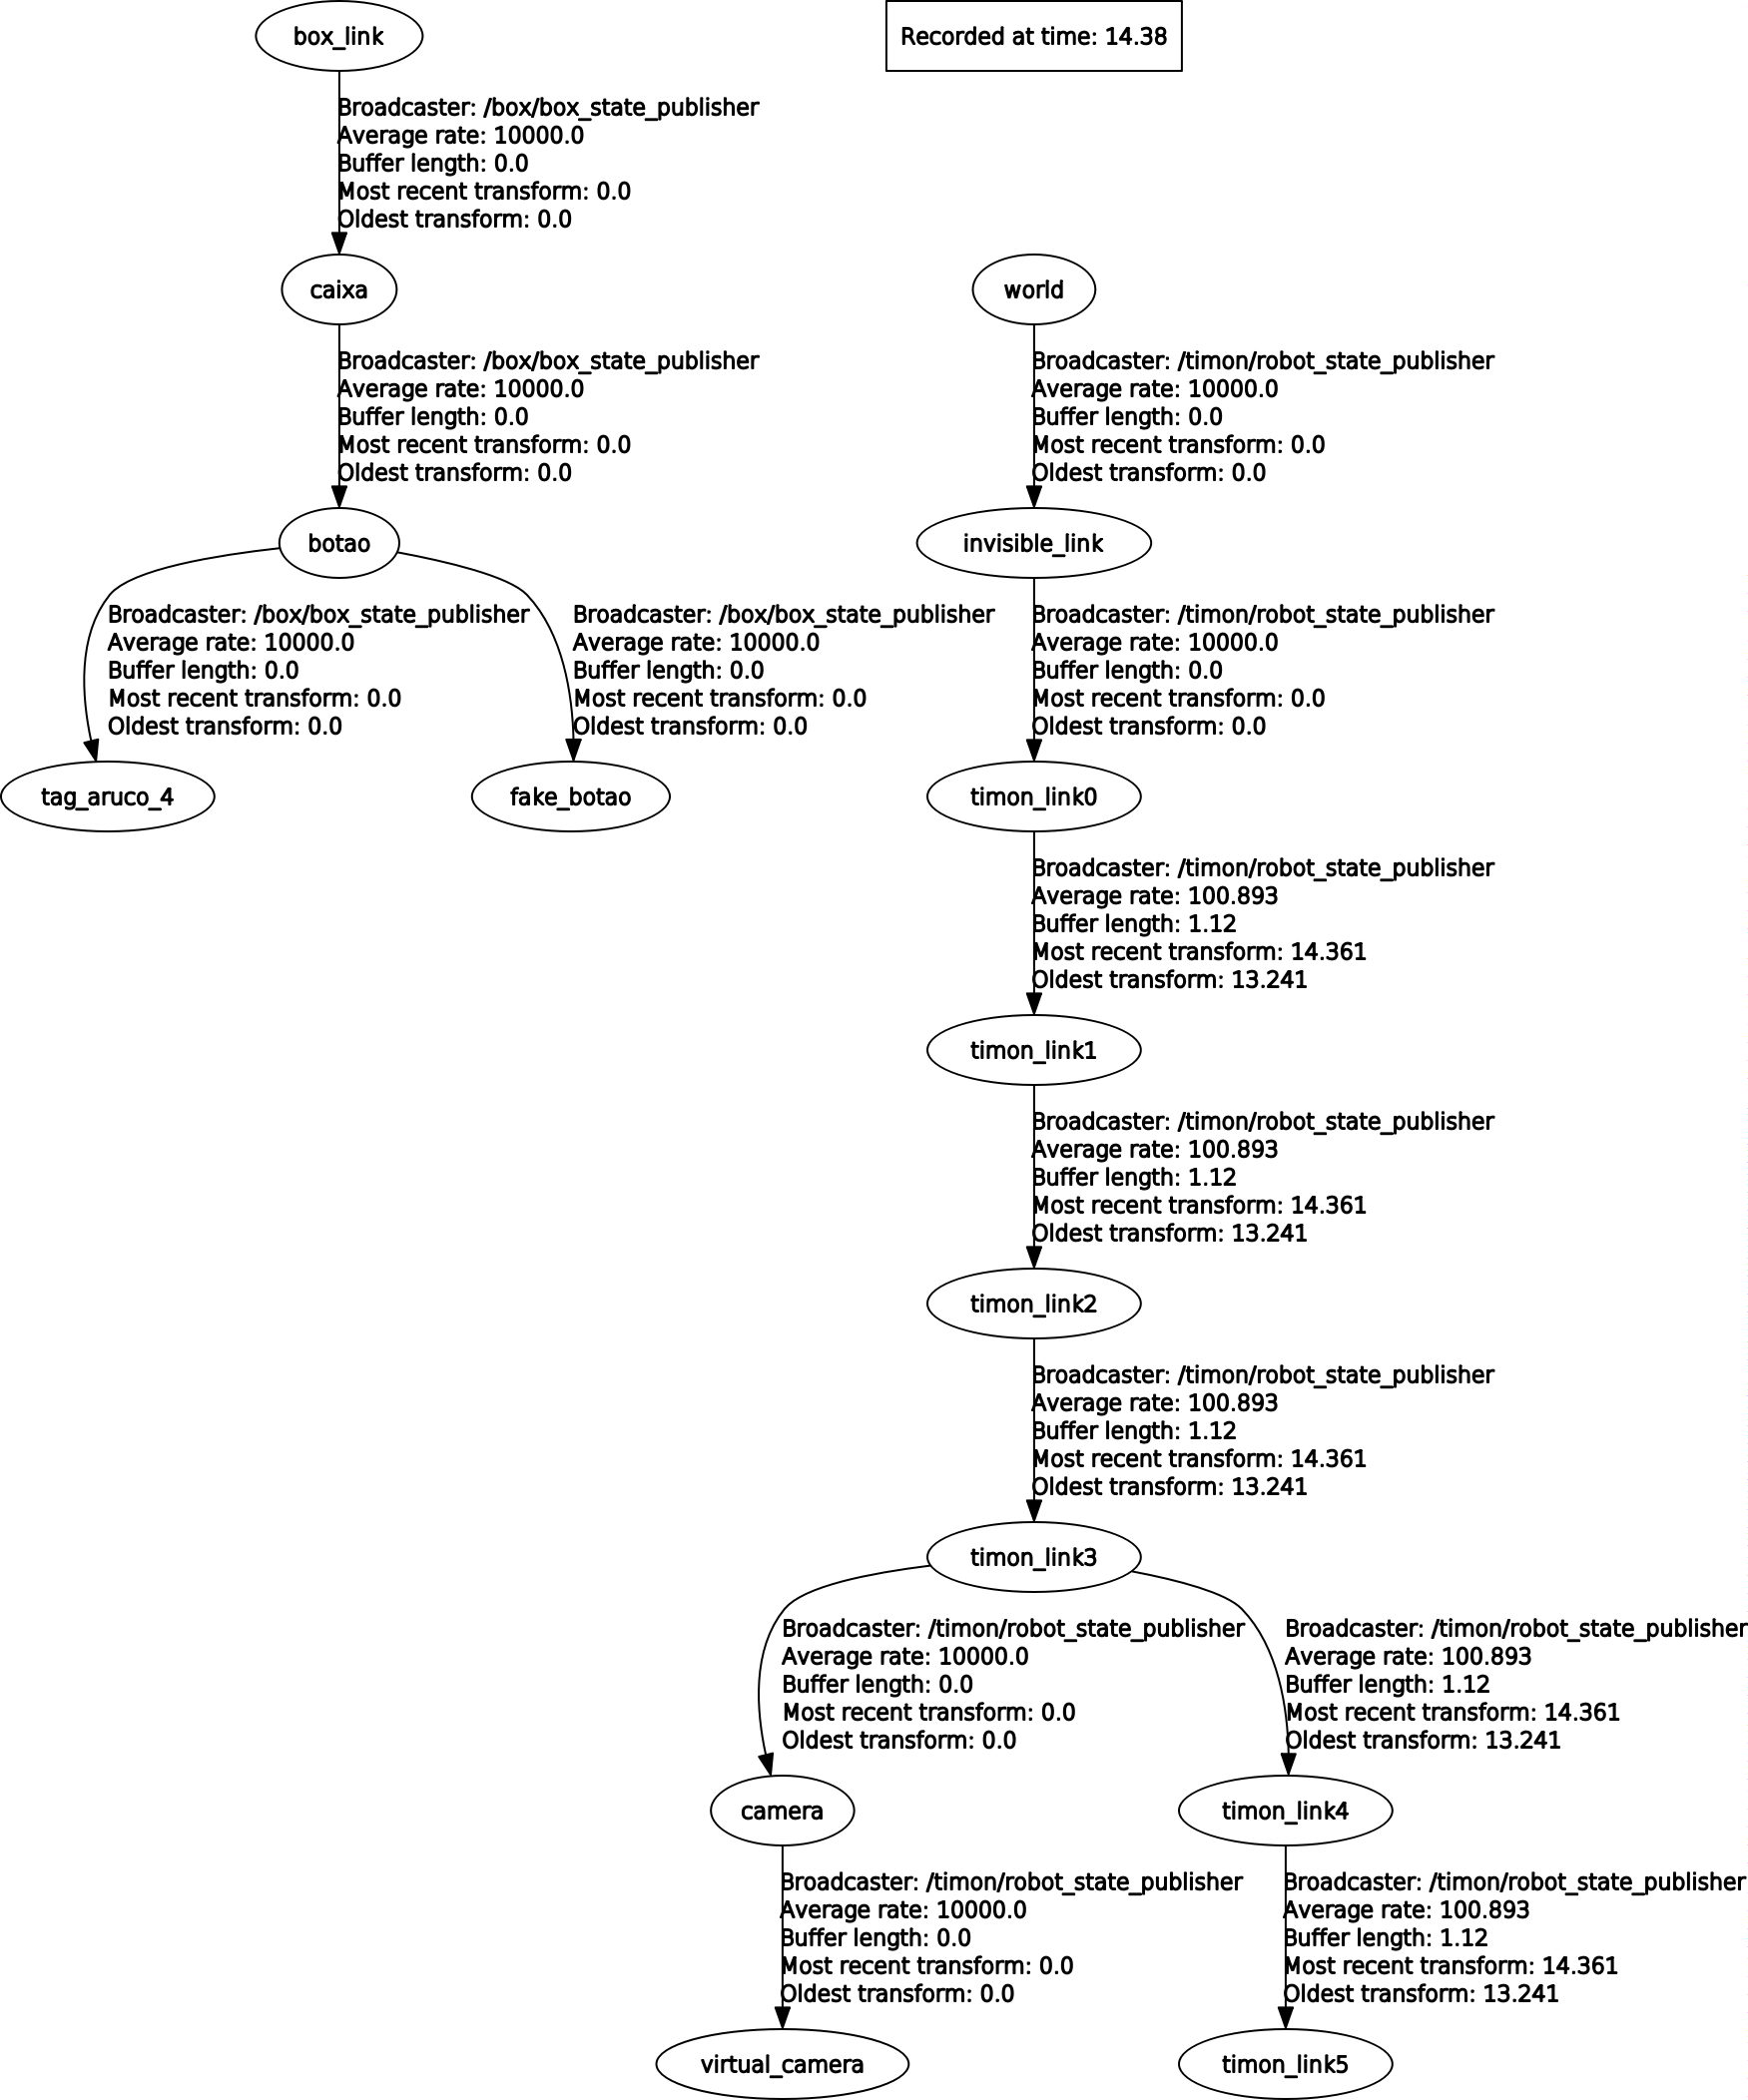
\includegraphics[scale=0.39]{appendix/tf_desconectadas.png}
		% \caption{Coordenadas.}
		% \label{fig:coordenadas}
	\end{figure}

	\chapter{Árvores de TF conectadas}
	\label{apend:tf2}
	\begin{figure}[H]
		\centering
		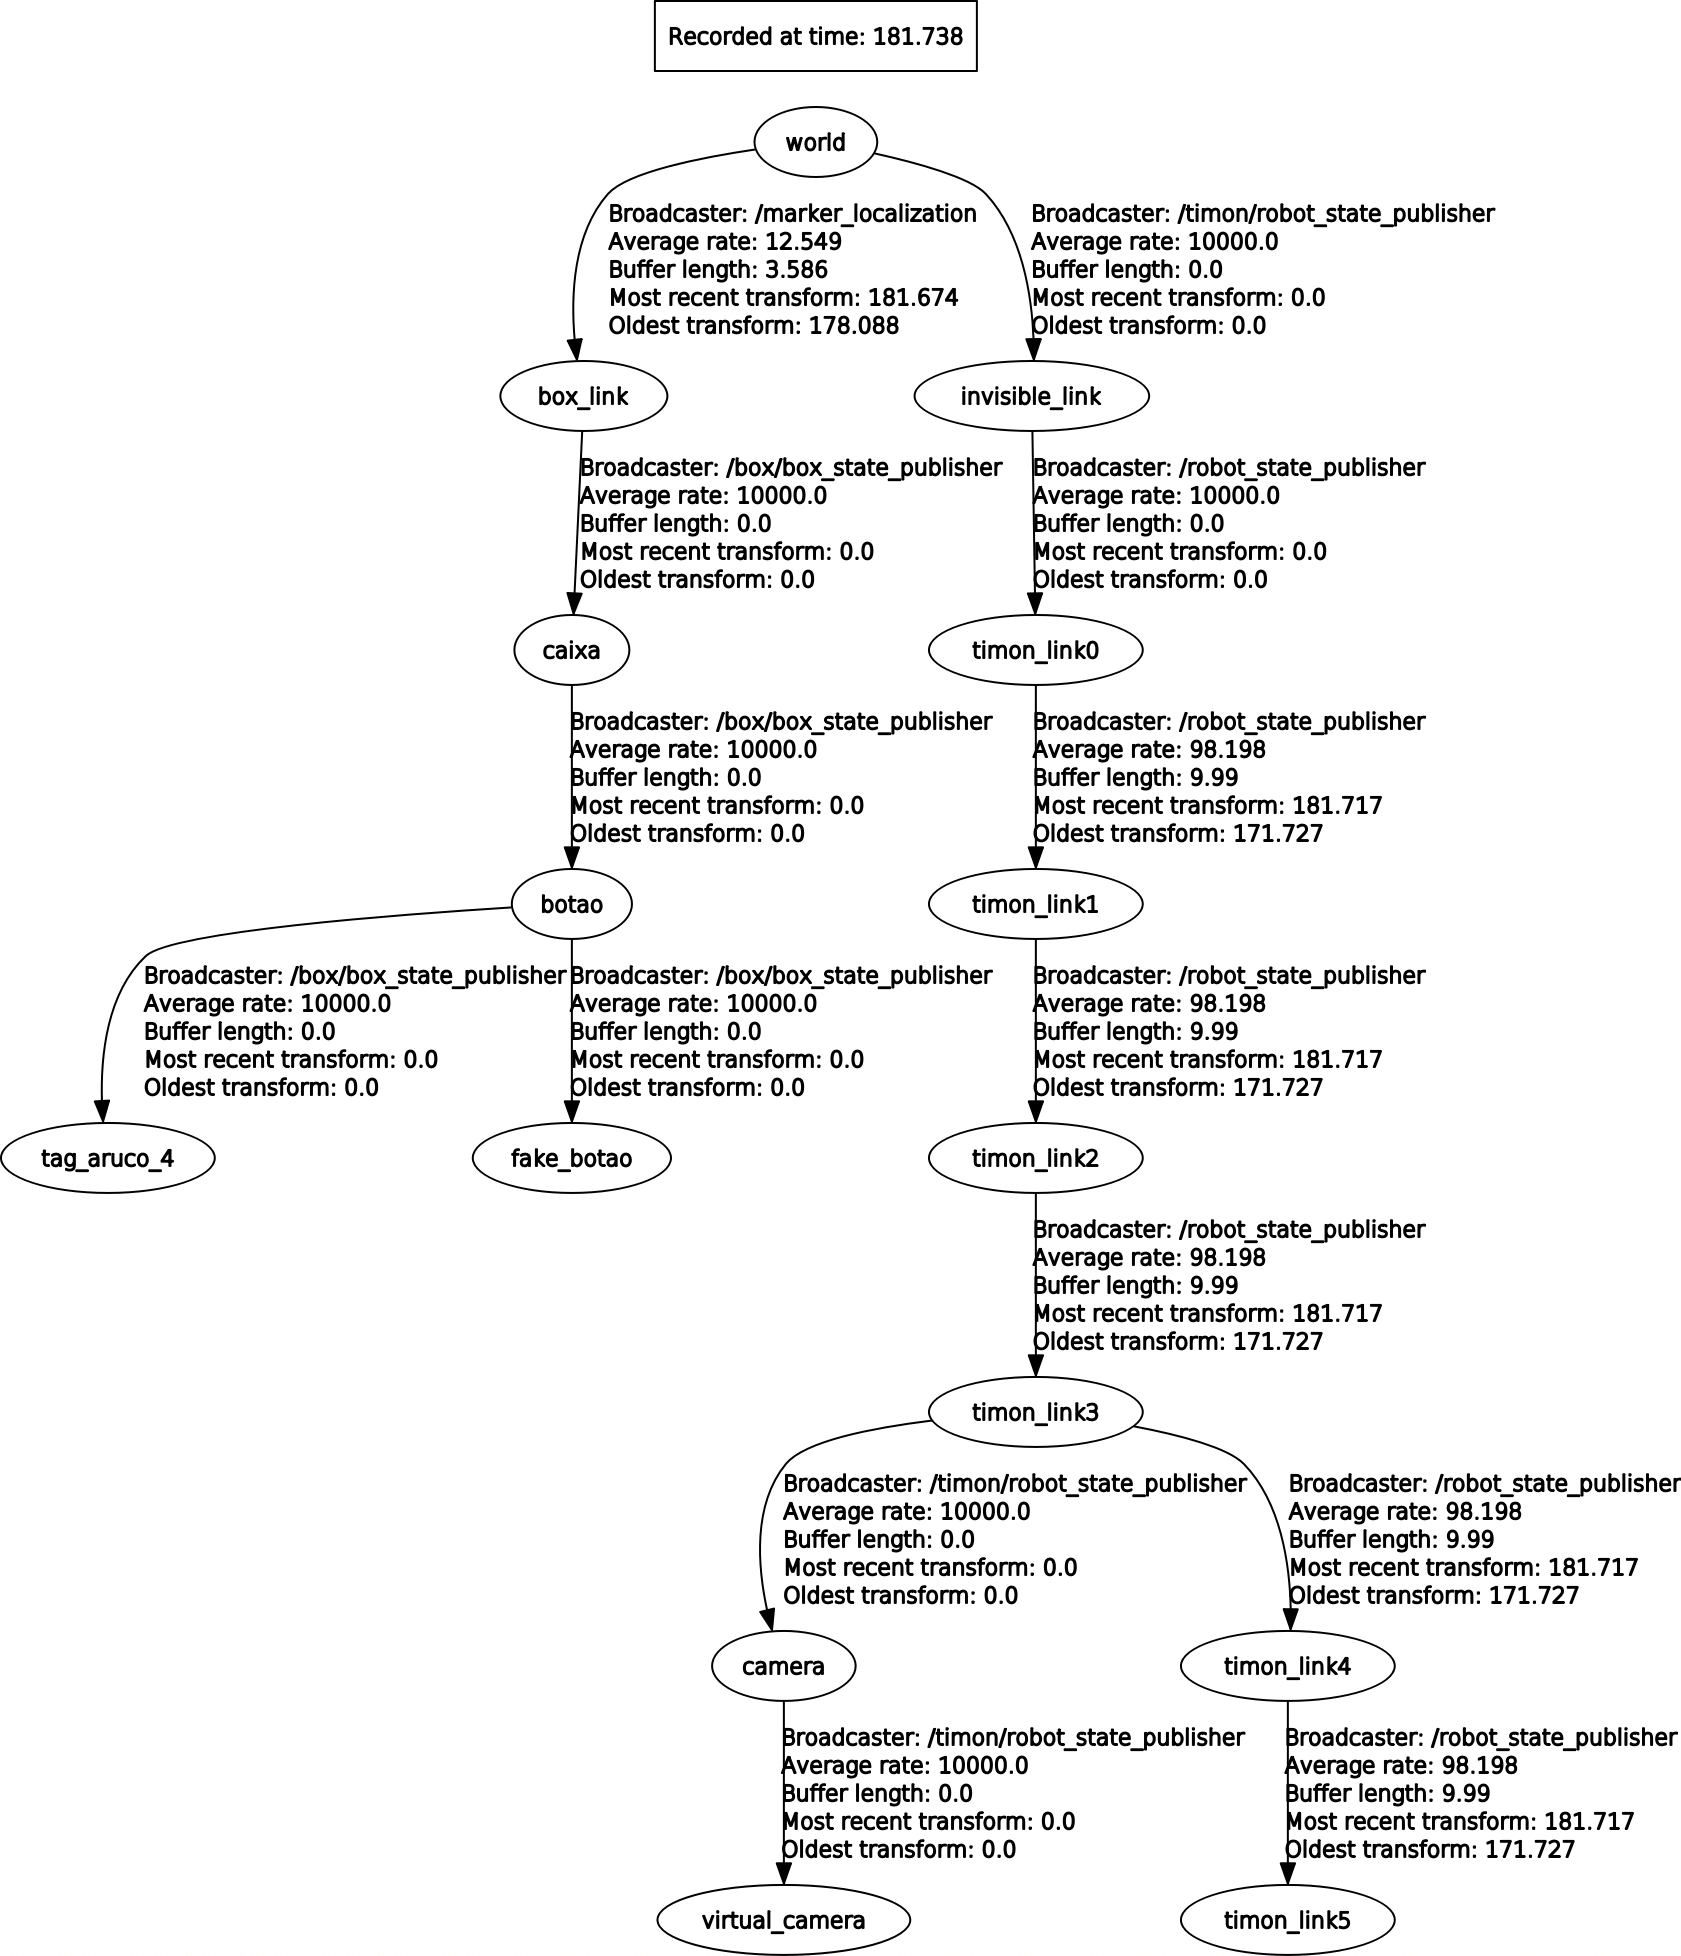
\includegraphics[scale=0.4]{appendix/tf_conectadas.png}
		% \caption{Coordenadas.}
		% \label{fig:coordenadas}
	\end{figure}

	\chapter{Diagrama de nós do sistema}
	\label{apend:rqt}
	\begin{figure}[H]
		\centering
		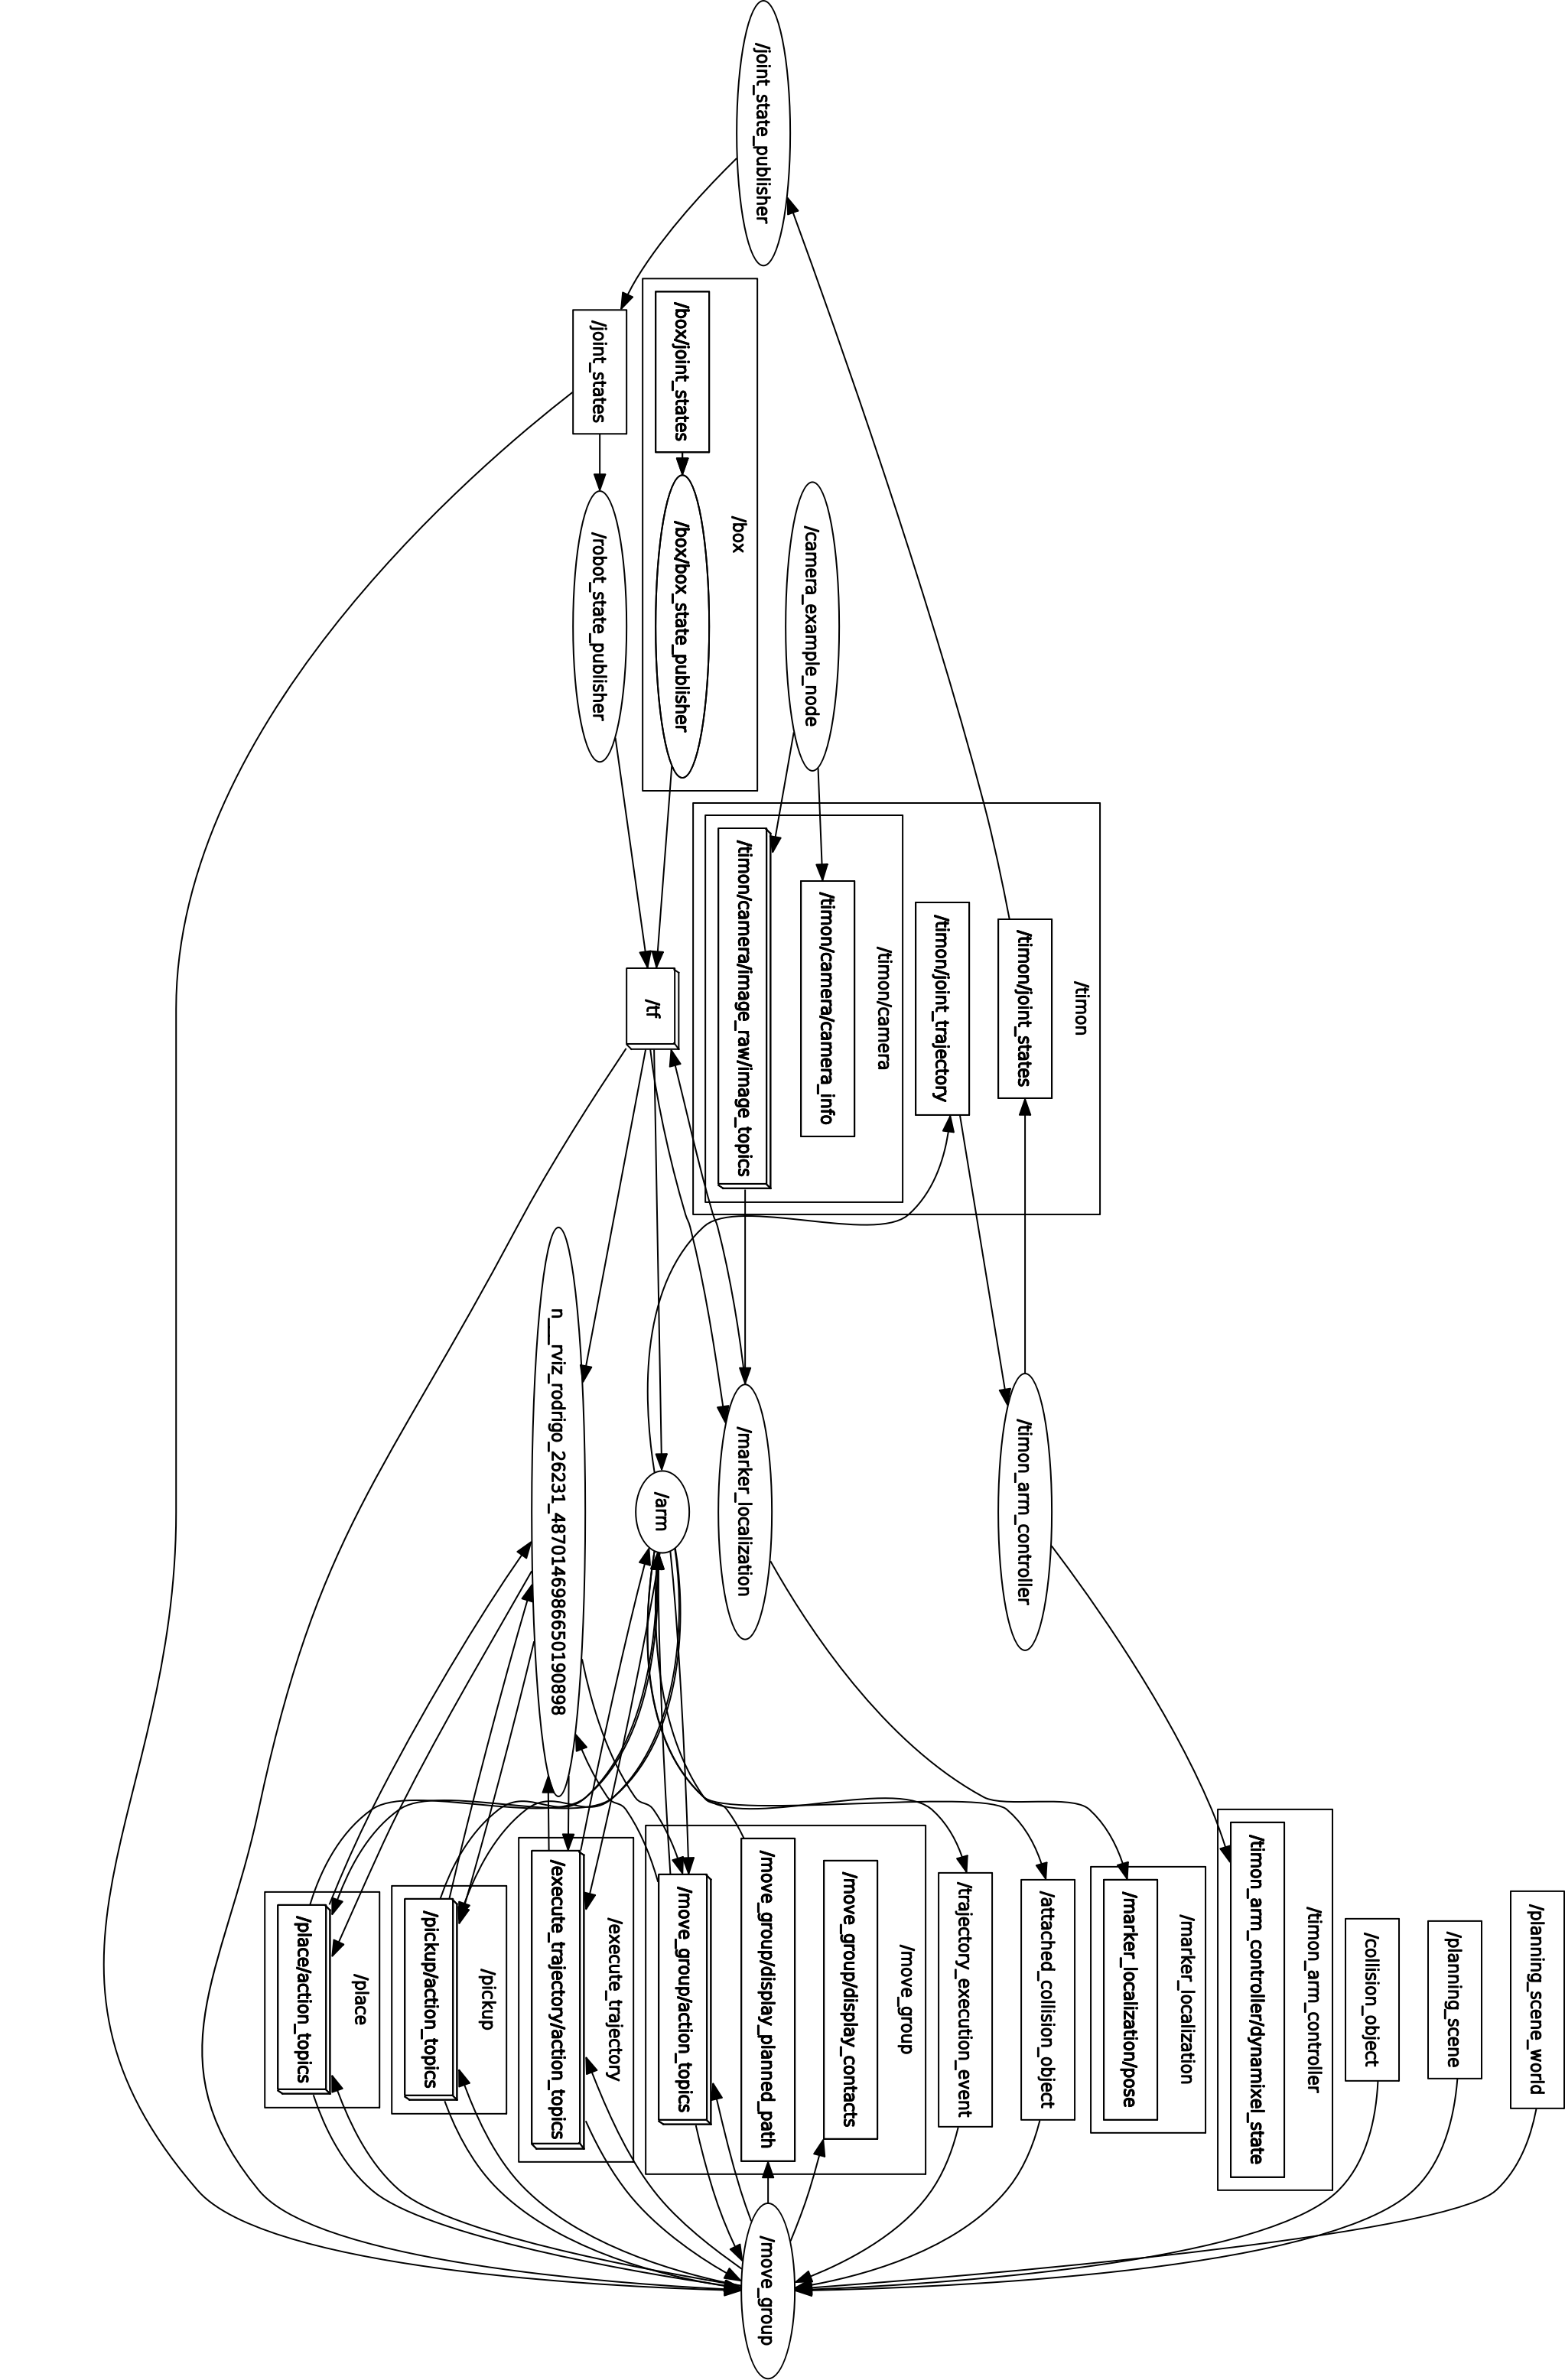
\includegraphics[scale=0.2]{appendix/rosgraph.png}
		% \caption{Coordenadas.}
		% \label{fig:coordenadas}
	\end{figure}

	
	\chapter{Propriedades de Massa do JeRoTIMON}
	\label{apend:quest}
	\begin{figure}[H]
		\centering
		\caption{Coordenadas.}
		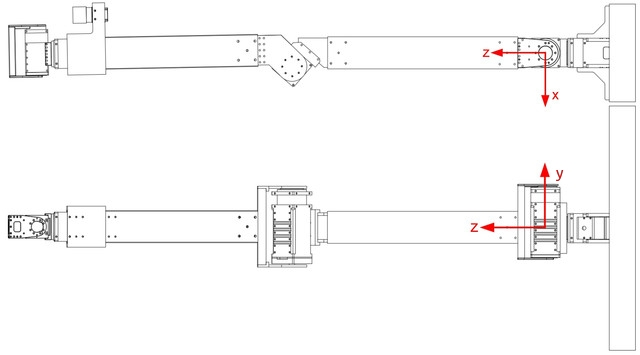
\includegraphics[scale=0.65]{appendix/coordinates.jpg}
		\label{fig:coordenadas}
	\end{figure}


	\begin{figure}[H]
		\centering
		\caption{Link 0.}
		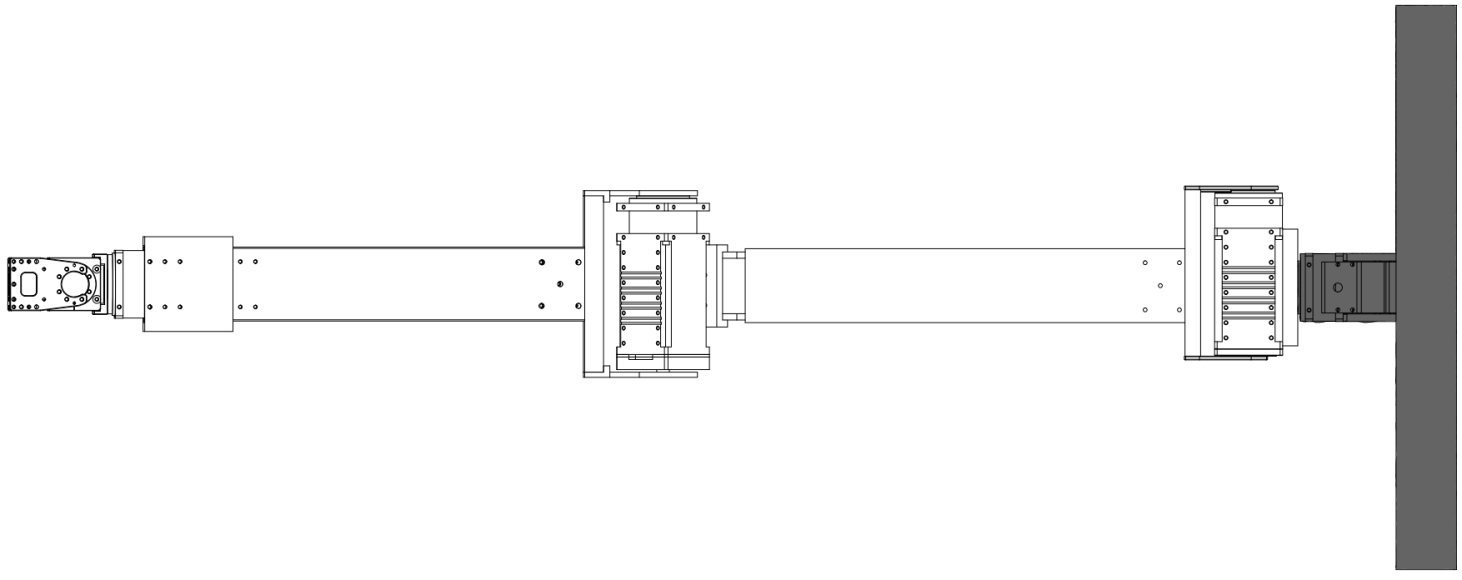
\includegraphics[scale=1.2]{appendix/link0.jpg}
		\label{fig:link0}
	\end{figure}

	\begin{itemize}
		\item \textbf{Massa:} $3.72384654$ kg
        \item \textbf{Volume:} $0.00413037 m^{3}$
		\item \textbf{Área:} $0.28622123 m^{2}$
		\item \textbf{Centro de  Massa:}
		\begin{itemize}
			\item X: $-0.00000147$ m
			\item Y: $0.00000000$ m
			\item Z: $0.03504069$ m
		\end{itemize}				
		\item \textbf{Momento de inércia:} kg $m^{2}$
		\begin{itemize}
			\item \textbf{Lxx:}	0.01072644 \textbf{Lxy:}-9.465e-9 \textbf{Lxz:}-3.247e-8				
			\item \textbf{Lyx:} -9.465e-9 \textbf{Lyy:} 0.04865651 \textbf{Lyz:} 6.830e-13					
			\item \textbf{Lzx:} -3.247e-8 \textbf{Lzy:} 6.830e-13 \textbf{Lzz:} 0.05388213					
		\end{itemize}		
	\end{itemize}

	\begin{figure}[H]
		\centering
		\caption{Link 1.}
		\includegraphics[scale=1.2]{appendix/link1.jpg}
		\label{fig:link1}
	\end{figure}

	\begin{itemize}
		\item \textbf{Massa:} $1.03781084$ kg
		\item \textbf{Volume:} $0.00040169$  $m^{3}$
		\item \textbf{Área:} $0.05853078$  $m^{2}$
		\item \textbf{Centro de  Massa:}
		\begin{itemize}
			\item X: $0.00814457$ m
			\item Y: $4.45597047e-8$ m
			\item Z: $0.16022275$ m
		\end{itemize}
		\item \textbf{Momento de inércia:} kg $m^{2}$
		\begin{itemize}
			\item \textbf{Lxx:}	0.0005687 \textbf{Lxy:} 2.602e-10 \textbf{Lxz:}	-0.00004027			
			\item \textbf{Lyx:} 2.602e-10 \textbf{Lyy:} 0.00166759 \textbf{Lyz:} -2.222e-10		
			\item \textbf{Lzx:} -0.00004027 \textbf{Lzy:} -2.222e-10 \textbf{Lzz:} 0.00155695			
		\end{itemize}	
	\end{itemize}
	

	\begin{figure}[H]
		\centering
		\caption{Link 2.}
		\includegraphics[scale=1.2]{appendix/link2.jpg}
		\label{fig:link2}
	\end{figure}

	\begin{itemize}
		\item \textbf{Massa:} $2.05026959$ kg		
		\item \textbf{Volume:} $0.00077667$ $m^{3}$
		\item \textbf{Área:} $0.29790369$ $m^{2}$
		\item \textbf{Centro de  Massa:}
		\begin{itemize}
			\item X: $0.00294129$ m			
			\item Y: $-0.01058166$ m			
			\item Z: $0.48960322$ m			
		\end{itemize}
		
		\item \textbf{Momento de inércia:} kg $m^{2}$
		\begin{itemize}
			\item \textbf{Lxx:} 0.06174738 \textbf{Lxy:} -0.00003476 \textbf{Lxz:} 0.00098626			
			\item \textbf{Lyx:} -0.00003476	\textbf{Lyy:} 0.06319525 \textbf{Lyz:} 0.00311701			 
			\item \textbf{Lzx:} 0.00098626 \textbf{Lzy:} 0.00311701 \textbf{Lzz:} 0.0034029			  
		\end{itemize}
	\end{itemize}
	

	\begin{figure}[H]
		\centering
		\caption{Link 3.}
		\includegraphics[scale=1.2]{appendix/link3.jpg}
		\label{fig:link3}
	\end{figure}

	\begin{itemize}
		\item \textbf{Massa:} $1.83580505$ kg		
		\item \textbf{Volume:} $0.00081683$ $m^{3}$
		\item \textbf{Área:} $0.32055793$ $m^{2}$
		\item \textbf{Centro de  Massa:}
		\begin{itemize}
			\item X: $0.00257384$ m
			\item Y: $0.00207951$ m
			\item Z: $0.91287054$ m			
		\end{itemize}
		
		\item \textbf{Momento de inércia:} kg $m^{2}$
		\begin{itemize}
			\item \textbf{Lxx:} 0.03439469 \textbf{Lxy:} -0.00000261 \textbf{Lxz:} -0.00001194			  
			\item \textbf{Lyx:} -0.00000261 \textbf{Lyy:} 0.03489631  \textbf{Lyz:} -0.0001288			  
			\item \textbf{Lzx:} -0.00001194 \textbf{Lzy:} -0.0001288 \textbf{Lzz:} 0.0023687			 
		\end{itemize}
	\end{itemize}

	\begin{figure}[H]
		\centering
		\caption{Link 4.}
		\includegraphics[scale=1.2]{appendix/link4.jpg}
		\label{fig:link4}
	\end{figure}

	\begin{itemize}
		\item \textbf{Massa:} $0.39425655$ kg
		\item \textbf{Volume:} $0.00014602$ $m^{3}$
		\item \textbf{Área:} $0.03018022$ $m^{2}$
		\item \textbf{Centro de  Massa:}
		\begin{itemize}
			\item X: $0.00257156$ m			
			\item Y: $0.00133073$ m			
			\item Z: $1.09673426$ m			
		\end{itemize}
		
		\item \textbf{Momento de inércia:} kg $m^{2}$
		\begin{itemize}
			\item \textbf{Lxx:}	0.00028795 \textbf{Lxy:} 2.010e-10 \textbf{Lxz:} -8.166e-13			  
			\item \textbf{Lyx:} 2.010e-10 \textbf{Lyy:} 0.00011981 \textbf{Lyz:} -0.00000446			  
			\item \textbf{Lzx:} -8.166e-13 \textbf{Lzy:} -0.00000446 \textbf{Lzz:} 0.0002842			  
		\end{itemize}
	\end{itemize}

	\begin{figure}[H]
		\centering
		\caption{Link 5.}
		\includegraphics[scale=1.2]{appendix/link5.jpg}
		\label{fig:link5}
	\end{figure}

	\begin{itemize}
		\item \textbf{Massa:} $0.08694786$ kg
		\item \textbf{Volume:} $0.0000322$ $m^{3}$
		\item \textbf{Área:} $0.02435944$ $m^{2}$
		\item \textbf{Centro de  Massa:}
		\begin{itemize}
			\item X: $0.00257155$ m			
			\item Y: $0.00684212$ m			
			\item Z: $1.13578562$ m
			
		\end{itemize}
		
		\item \textbf{Momento de inércia:} kg $m^{2}$
		\begin{itemize}
			\item \textbf{Lxx:}	0.00012963 \textbf{Lxy:} -5.235e-13  \textbf{Lxz:} -9.996e-14			   
			\item \textbf{Lyx:} -5.235e-13 \textbf{Lyy:} 0.00003703 \textbf{Lyz:} 0.00000247			   
			\item \textbf{Lzx:} -9.996e-14 \textbf{Lzy:} 0.00000247	 \textbf{Lzz:} 0.00012613			 
		\end{itemize}
	\end{itemize}

	\chapter{Lista de suportes.}
	\label{apend:frames}

	\begin{table}[H]
		\caption{Tabela de suportes}
		\begin{adjustbox}{max width=\textwidth}
		\begin{tabular}{|c|c|c|c|c|c|c|}
		\hline
		\rowcolor[HTML]{EFEFEF} 
		Imagem                 & Junta & Fornecedor     & Tipo                & Modelo               & Quantidade & Medidas (mm)          \\ \hline
		\includegraphics[scale=0.12]{appendix/cantoneira.png}          & Id\_1 & CCRoSA         & Cantoneira          & Original             & 2          & 59 x 59 x 40.5        \\ \hline
		\rowcolor[HTML]{EFEFEF} 
		\includegraphics[scale=0.12]{appendix/ffixper1.png}               & Id\_2 & CCRoSA         & Frame Perpendicular & Original             & 1          & 92.6 x 51.1 x 12      \\ \hline
		\includegraphics[scale = 0.12]{appendix/fr54.png}            & Id\_2 & ROBOTIS        & Rolamento           & FRP54-I110K          & 1          & 54 x 54 x 5           \\ \hline
		\rowcolor[HTML]{EFEFEF} 
		\includegraphics[scale = 0.12]{appendix/frot1.png}       & Id\_3 & ROBOTIS/CCRoSA & Frame de Rotação    & FRP54-H221K/Original & 1          & 105.5 x 138 x 54.3    \\ \hline
		\includegraphics[scale=0.12]{appendix/fix2.png}       & Id\_3 & CCRoSA         & Fixador             & Original             & 1          & 95 x 54 x 54          \\ \hline
		\rowcolor[HTML]{EFEFEF} 
		\includegraphics[scale = 0.12]{appendix/fix22.png}     & Id\_3 & CCRoSA         & Fixador             & Original             & 1          & 60 x 65.2 x 17        \\ \hline
		\includegraphics[scale=0.12]{appendix/calco.png}                 & Id\_3 & CCRoSA         & Calço               & Original             & 1          & 54 x 54 x 2           \\ \hline
		\rowcolor[HTML]{EFEFEF} 
		\includegraphics[scale = 0.12]{appendix/rolamentoorigi.png}        & Id\_3 & CCRoSA         & Rolamento           & Original             & 1          & 54 x 54 x 10          \\ \hline
		\includegraphics[scale = 0.12]{appendix/frot2.png}      & Id\_4 & CCRoSA         & Frame de Rotação    & Original             & 1          & 85.03 x 89.46 x 148.2 \\ \hline
		\rowcolor[HTML]{EFEFEF} 
		\includegraphics[scale = 0.12]{appendix/ffixper.png} & Id\_5 & ROBOTIS        & Frame Perpendicular & FRP42-A110K          & 1          & 48 x 42 x 11.5        \\ \hline
		\includegraphics[scale = 0.12]{appendix/rolamento42.png}           & Id\_5 & ROBOTIS        & Rolamento           & FRP42-I110K          & 1          & 42 x 42 x 5           \\ \hline
		\rowcolor[HTML]{EFEFEF} 
		\includegraphics[scale = 0.12]{appendix/frot3.png}       & Id\_6 & ROBOTIS        & Frame de Rotação    & FRP42-H121K          & 1          & 96 x 42 x 56.6        \\ \hline
		\end{tabular}
		\end{adjustbox}
		\caption*{Fonte: Adaptado de \cite{dynamixel}}
		\label{appen:lista_supor}
		\end{table}
	\chapter{Projeto mecânico}
	\label{apend:proj_mec}
	
	O projeto mecânico do manipulador JeRoTIMON foi desenvolvido em duas etapas: Modelagem 3D e Cálculos Estáticos. A etapa de modelagem levou em consideração, além da análise estrutural e requisitos do cliente, as restrições físicas para que o manipulador pudesse ser anexado no UGV \textit{Warthog}. Por fim, foi realizado os cálculos de esforços estáticos em que analisou-se os esforços sofridos pelo manipulador, na situação em que exige uma maior carga dos atuadores, e com isso garanta a funcionalidade do mesmo. A seguir, será visto o desenho mecânico final do manipulador e como foi realizado a análise estática.

	\section{Desenho mecânico}
	O desenho do manipulador foi todo elaborado utilizando o \textit{software ``OnShape''}. A Figura \ref{des:3_vis} mostra o desenho técnico do manipulador com as vistas: frontal, lateral esquerda, superior e isométrica, contendo todos os detalhes necessários para execução do projeto. A figura \ref{des:iso} mostra a vista isométrica expandida do manipulador em sua posição \textit{home}.

	\begin{figure}[H]
		\centering
		\caption{Desenho técnico do JeRoTIMON, vistas: frontal, lateral esquerda e superior.}
		\includegraphics[scale=.55, angle=90]{appendix/3_vistas.png}
		\caption*{Fonte: Autoria própria.}
		\label{des:3_vis}
	\end{figure}

	\begin{figure}[H]
		\centering
		\caption{Desenho técnico do JeRoTIMON, vista isométrica.}
		\includegraphics[scale=.55, angle=90]{appendix/isometrica.png}
		\caption*{Fonte: Autoria própria.}
		\label{des:iso}
	\end{figure}

	\section{Analise estática}

	Para calcular a carga máxima suportada pelo manipulador foi realizada uma análise estática. Para isso, o mesmo foi posto na situação em que exige um maior esforço das juntas 0 e 1, conforme visto na Figura \ref{fig:esfoco}.

	\begin{figure}[H]
		\centering
		\caption{Analise estática - condição de maior esforço exigido.}
		\includegraphics[width=1\textwidth]{appendix/esforcos.png}
		\caption*{fonte: Autoria Própria}
		\label{fig:esfoco}
	\end{figure}

	Para analisar os esforços sofridos pela junta 1 (motor 2), admiti-se a extremidade esquerda como engastada e em sua situação de equilíbrio estático, como visto na Figura \ref{fig:esfoco}. A força resultante no eixo y é calculada da seguinte forma: 
	$$ \sum F_{r_{y}} = 0 $$
	$$F_{r_{y}} - 4,04 - 4,44 - 15,3 - 4,44 - 17 = 0$$
	$$ F_{r_{y}} = \textbf{45,22 [N]}  $$

	Para calcular o torque sofrido pela junta, as cargas distribuídas de cada componente do robô foram colocadas no seu centróide, conforme visto na Figura \ref{fig:esfoco_m}. 

	\begin{figure}[H]
		\centering
		\caption{Analise estática - condição de maior esforço exigido (cargas no centróide).}
		\includegraphics[width=1\textwidth]{appendix/esforcom.png}
		\caption*{fonte: Autoria Própria}
		\label{fig:esfoco_m}
	\end{figure}

	Em seguida, foi calculado o momento torsor gerado nos motores 1 e 2 por cada carga pontual da seguinte maneira: 

	$$\sum M_{r} = 0 $$
	$$M_{r} - (4,04\times0,05) - (4,44\times0,23) - (15,3\times0,41) - (4,44\times0,71) - (17\times0,89) = 0$$
	$$M_{r} = \textbf{25,8 [N x m]} $$

	Por fim, foi calculada a carga máxima suportada pelo manipulador, também conhecida por \textit{payload}. Para este cálculo, foi necessário obter e comparar as informações sobre o torque máximo fornecido pelo motor que compõe a junta 1 (PH54-200-S500-R) que é de 44,7 N x m, segundo o \textit{datasheet} disponível no anexo \ref{ann:esp_motors_ph54_200}. Sendo o alcance máximo de 0,89 m, temos:
	$$T_{max/motor}= T_{sofrido} - T{payload}$$
	$$44,7 = 25,8 - (F_{payload}\times0,89)$$
	$$F_{payload}= 21,23 [N]$$

	De acordo com a Segunda Lei de Newton e considerando a aceleração da gravidade como 10 $m/s^{2}$, obtemos uma carga máxima suportada pelo manipulador de:
	$$F_{r} = m \times a $$
	$$21,23 = m \times 10$$
	$$m = \textbf{2,1 [kg]}$$



	\chapter{Algoritmo de busca e acionamento do painel}
	\label{apend:algorit}

	
	\lstinputlisting[language=C++, inputencoding=utf8/latin1, showspaces =false,	showstringspaces=false, breaklines=true, label=fonte, frame=single]{appendix/push_button.cpp}

	
	\chapter{Diagrama elétrico do JeRoTIMON}
	\label{apend:diag_ele}
	\begin{figure}[H]
		\centering
		\includegraphics[scale=0.72]{appendix/wiring_1.png}
		\label{fig:wiring1}
	\end{figure}

	\begin{figure}[H]
		\centering
		\includegraphics[scale=0.72]{appendix/wiring_2.png}
		\label{fig:wiring2}
	\end{figure}

	\begin{figure}[H]
		\centering
		\includegraphics[scale=0.72]{appendix/wiring_3.png}
		\label{fig:wiring3}
	\end{figure}

	\begin{figure}[H]
		\centering
		\includegraphics[scale=0.72]{appendix/wiring_4.png}
		\label{fig:wiring4}
	\end{figure}

	\begin{figure}[H]
		\centering
		\includegraphics[scale=0.72]{appendix/wiring_5.png}
		\label{fig:wiring5}
	\end{figure}

	\begin{figure}[H]
		\centering
		\includegraphics[scale=0.72]{appendix/wiring_6.png}
		\label{fig:wiring6}
	\end{figure}

	\begin{figure}[H]
		\centering
		\includegraphics[scale=0.72]{appendix/wiring_7.png}
		\label{fig:wiring7}
	\end{figure}


	\chapter{Diagrama de conexão do JeRoTIMON}
	\label{apend:connec_schem}
	\begin{figure}[H]
		\centering
		\includegraphics[scale=0.72]{appendix/connection_1.png}
		\label{fig:connection1}
	\end{figure}

	\begin{figure}[H]
		\centering
		\includegraphics[scale=0.72]{appendix/connection_2.png}
		\label{fig:connection2}
	\end{figure}

	\begin{figure}[H]
		\centering
		\includegraphics[scale=0.72]{appendix/connection_3.png}
		\label{fig:connection3}
	\end{figure}

	\begin{figure}[H]
		\centering
		\includegraphics[scale=0.72]{appendix/connection_4.png}
		\label{fig:connection4}
	\end{figure}

	\begin{figure}[H]
		\centering
		\includegraphics[scale=0.72]{appendix/connection_5.png}
		\label{fig:connection5}
	\end{figure}

	

	%\includepdf[pages={{},-}]{appendix/listquest.pdf}
	%\lipsum[1] % Comentar e adicionar apêndice aqui
	%
	%\chapter{Um assunto importante}
	%\label{apend:assunto}
	%\lipsum[1] % Comentar e adicionar apêndice aqui
	

% --------------------------------------------------------------------------
% Anexos                                                                     
	\anexos
	\justify
	%
	\chapter{Especificações da câmera Dalsa Genie Nano}
	\label{ann:relant}
	
	\includepdf[pages={1-3}]{annex/genie_nano.pdf}

	\chapter{Especificações do motor \textit{Dynamixel} PH42-020-S300-R}
	\label{ann:esp_motors_hp42}

	\begin{table}[H]
		\begin{adjustbox}{max width=\textwidth}
		\begin{tabular}{|c|c|}
		\hline
		\rowcolor[HTML]{EFEFEF} 
		\textbf{Item}                                                                               & \textbf{Especificação}                                                                          \\ \hline
		\rowcolor[HTML]{FFFFFF} 
		{\color[HTML]{000000} \textbf{Microcontrolador}}                                            & {\color[HTML]{000000} ARM CORTEX-M4 (168 {[}MHz{]}, 32Bit)}                                     \\ \hline
		\rowcolor[HTML]{EFEFEF} 
		{\color[HTML]{000000} \textbf{Motor}}                                                       & {\color[HTML]{000000} Coreless (Maxon)}                                                         \\ \hline
		\rowcolor[HTML]{FFFFFF} 
		{\color[HTML]{000000} \textbf{Taxa de transmissão}}                                         & {\color[HTML]{000000} 9,600 {[}bps{]} $\sim$10.5 {[}Mbps{]}}                                    \\ \hline
		\rowcolor[HTML]{EFEFEF} 
		\cellcolor[HTML]{EFEFEF}{\color[HTML]{000000} }                                             & {\color[HTML]{000000} Torque Control Mode}                                                      \\ \cline{2-2} 
		\rowcolor[HTML]{EFEFEF} 
		\cellcolor[HTML]{EFEFEF}{\color[HTML]{000000} }                                             & {\color[HTML]{000000} Velocity Control Mode}                                                    \\ \cline{2-2} 
		\rowcolor[HTML]{EFEFEF} 
		\cellcolor[HTML]{EFEFEF}{\color[HTML]{000000} }                                             & {\color[HTML]{000000} Position Control Mode}                                                    \\ \cline{2-2} 
		\rowcolor[HTML]{EFEFEF} 
		\cellcolor[HTML]{EFEFEF}{\color[HTML]{000000} }                                             & {\color[HTML]{000000} Extended Position Control Mode}                                           \\ \cline{2-2} 
		\rowcolor[HTML]{EFEFEF} 
		\multirow{-5}{*}{\cellcolor[HTML]{EFEFEF}{\color[HTML]{000000} \textbf{Modos de operação}}} & {\color[HTML]{000000} PWM Control Mode (Voltage Control Mode)}                                  \\ \hline
		\rowcolor[HTML]{FFFFFF} 
		{\color[HTML]{000000} \textbf{Massa}}                                                       & {\color[HTML]{000000} 340 {[}g{]}}                                                              \\ \hline
		\rowcolor[HTML]{EFEFEF} 
		{\color[HTML]{000000} \textbf{Dimensões (L x A x P)}}                                       & {\color[HTML]{000000} 42 x 84 x 42 {[}mm{]}}                                                    \\ \hline
		\rowcolor[HTML]{FFFFFF} 
		{\color[HTML]{000000} \textbf{Resolução}}                                                   & {\color[HTML]{000000} 607,500 {[}pulsos/rev{]}}                                                 \\ \hline
		\rowcolor[HTML]{EFEFEF} 
		{\color[HTML]{000000} \textbf{Relação de transmissão}}                                      & {\color[HTML]{000000} 303.75:1}                                                                 \\ \hline
		\rowcolor[HTML]{FFFFFF} 
		{\color[HTML]{000000} \textbf{Folga}}                                                       & {\color[HTML]{000000} \textless 6 {[}arcmin{]}, 0.1 {[}$^\circ${]}}                             \\ \hline
		\rowcolor[HTML]{EFEFEF} 
		{\color[HTML]{000000} \textbf{Carga radial}}                                                & {\color[HTML]{000000} 280 {[}N{]} (10 {[}mm{]} afastado da face do eixo)}                       \\ \hline
		\rowcolor[HTML]{FFFFFF} 
		{\color[HTML]{000000} \textbf{Carga axial}}                                                 & {\color[HTML]{000000} 100 {[}N{]}}                                                              \\ \hline
		\rowcolor[HTML]{EFEFEF} 
		{\color[HTML]{000000} \textbf{Velocidade sem carga}}                                        & {\color[HTML]{000000} 32.7 {[}rev/min{]}}                                                       \\ \hline
		\rowcolor[HTML]{FFFFFF} 
		{\color[HTML]{000000} \textbf{Corrente sem carga}}                                          & {\color[HTML]{000000} 0.57 {[}A{]}}                                                             \\ \hline
		\rowcolor[HTML]{EFEFEF} 
		{\color[HTML]{000000} \textbf{Velocidade contínua}}                                         & {\color[HTML]{000000} 29.2 {[}rev/min{]}}                                                       \\ \hline
		\rowcolor[HTML]{FFFFFF} 
		{\color[HTML]{000000} \textbf{Torque contínuo}}                                             & {\color[HTML]{000000} 5.1 {[}Nm{]}}                                                             \\ \hline
		\rowcolor[HTML]{EFEFEF} 
		{\color[HTML]{000000} \textbf{Corrente contínua}}                                           & {\color[HTML]{000000} 1.5 {[}A{]}}                                                              \\ \hline
		\rowcolor[HTML]{FFFFFF} 
		{\color[HTML]{000000} \textbf{Potência de saída}}                                           & {\color[HTML]{000000} 20 {[}W{]}}                                                               \\ \hline
		\rowcolor[HTML]{EFEFEF} 
		{\color[HTML]{000000} \textbf{Temperatura de operação}}                                     & {\color[HTML]{000000} 5 $\sim$55 {[}$^\circ$C{]}}                                               \\ \hline
		\rowcolor[HTML]{FFFFFF} 
		{\color[HTML]{000000} \textbf{Tensão de operação}}                                          & {\color[HTML]{000000} 24.0 {[}V{]}}                                                             \\ \hline
		\rowcolor[HTML]{EFEFEF} 
		{\color[HTML]{000000} \textbf{Sinal de comando}}                                            & {\color[HTML]{000000} Pacotes digitais}                                                         \\ \hline
		\rowcolor[HTML]{FFFFFF} 
		{\color[HTML]{000000} \textbf{Protocolo de comunicação}}                                    & {\color[HTML]{000000} RS485 Comunicação serial asíncrona (8bit, 1 bit de parada, sem paridade)} \\ \hline
		\rowcolor[HTML]{EFEFEF} 
		{\color[HTML]{000000} \textbf{Conexão física}}                                              & {\color[HTML]{000000} RS485 Barramento multiponto}                                              \\ \hline
		\rowcolor[HTML]{FFFFFF} 
		{\color[HTML]{000000} \textbf{ID}}                                                          & {\color[HTML]{000000} 253 ID (0 $\sim$252)}                                                     \\ \hline
		\rowcolor[HTML]{EFEFEF} 
		{\color[HTML]{000000} \textbf{Corrente de espera}}                                          & {\color[HTML]{000000} 80 {[}mA{]}}                                                              \\ \hline
		\end{tabular}
		\end{adjustbox}
		\caption{Especificações do motor \textit{Dynamixel} HP42-020-S300-R}
		\end{table}
	% \begin{table}[H]
	% 	\begin{adjustbox}{max width=\textwidth}
	% 	\begin{tabular}{|c|c|}
	% 	\hline
	% 	\rowcolor[HTML]{EFEFEF} 
	% 	{\color[HTML]{000000} \textbf{Item}}                             & {\color[HTML]{000000} \textbf{Especificações}}                                           \\ \hline
	% 	\rowcolor[HTML]{FFFFFF} 
	% 	\textit{MCU}                                                     & \textit{ARM CORTEX-M3 (72 {[}MHz{]}, 32 Bit)}                                            \\ \hline
	% 	\rowcolor[HTML]{EFEFEF} 
	% 	\cellcolor[HTML]{EFEFEF}                                         & Enconder absoluto (sem contato) (12 Bit, 360 {[}$^ \circ ${])}                    \\ \cline{2-2} 
	% 	\rowcolor[HTML]{EFEFEF} 
	% 	\multirow{-2}{*}{\cellcolor[HTML]{EFEFEF}Sensor de posição}      & Fabricante: \href{www.ams.com}{AMS}, Numero da peça : AS5045 \\ \hline
	% 	\rowcolor[HTML]{FFFFFF} 
	% 	Motor                                                            & \textit{Coreless (Maxon)}                                                                \\ \hline
	% 	\rowcolor[HTML]{EFEFEF} 
	% 	Taxa de transmissão                                              & 8,000 {[}bps{]} $\sim$4.5 {[}Mbps{]}                                                     \\ \hline
	% 	\rowcolor[HTML]{FFFFFF} 
	% 	Algoritmo de controle                                            & Controle PID                                                                             \\ \hline
	% 	\rowcolor[HTML]{EFEFEF} 
	% 	Resolução                                                        & 4096 {[}pulse/rev{]}                                                                     \\ \hline
	% 	\rowcolor[HTML]{FFFFFF} 
	% 	Folga                                                            & 20 {[}arcmin{]} (0.33 {[}$^\circ${]})                                                    \\ \hline
	% 	\rowcolor[HTML]{EFEFEF} 
	% 	Modo operacional                                                 & Modo junta (0 $\sim$ 360 {[}$^\circ${]}) Modo roda (Curso sem fim)                       \\ \hline
	% 	\rowcolor[HTML]{FFFFFF} 
	% 	Peso                                                             & 165 {[}g{]}                                                                              \\ \hline
	% 	\rowcolor[HTML]{EFEFEF} 
	% 	Dimensões (c x l x h)                                            & 40.2 x 65.1 x 46 {[}mm{]}                                                                \\ \hline
	% 	\rowcolor[HTML]{FFFFFF} 
	% 	Relação de engrenagem                                            & 225 : 1                                                                                  \\ \hline
	% 	\rowcolor[HTML]{EFEFEF} 
	% 	\cellcolor[HTML]{EFEFEF}                                         & 8.0 {[}Nm{]} (at 11.1 {[}V{]}, 4.8 {[}A{]})                                              \\ \cline{2-2} 
	% 	\rowcolor[HTML]{EFEFEF} 
	% 	\cellcolor[HTML]{EFEFEF}                                         & 8.4 {[}Nm{]} (at 12.0 {[}V{]}, 5.2 {[}A{]})                                              \\ \cline{2-2} 
	% 	\rowcolor[HTML]{EFEFEF} 
	% 	\multirow{-3}{*}{\cellcolor[HTML]{EFEFEF}Torque de Parada}       & 10.0 {[}Nm{]} (at 14.8 {[}V{]}, 6.3 {[}A{]})                                             \\ \hline
	% 	\rowcolor[HTML]{FFFFFF} 
	% 	\cellcolor[HTML]{FFFFFF}                                         & 41 {[}rev/min{]} (at 11.1 {[}V{]})                                                       \\ \cline{2-2} 
	% 	\rowcolor[HTML]{FFFFFF} 
	% 	\cellcolor[HTML]{FFFFFF}                                         & 45 {[}rev/min{]} (at 12.0 {[}V{]})                                                       \\ \cline{2-2} 
	% 	\rowcolor[HTML]{FFFFFF} 
	% 	\multirow{-3}{*}{\cellcolor[HTML]{FFFFFF}Velocidade (sem carga)} & 55 {[}rev/min{]} (at 14.8 {[}V{]})                                                       \\ \hline
	% 	\rowcolor[HTML]{EFEFEF} 
	% 	Carga radial                                                     & 40 {[}N{]} (10 {[}mm{]} afastado da face do eixo)                                        \\ \hline
	% 	\rowcolor[HTML]{FFFFFF} 
	% 	Carga axial                                                      & 20 {[}N{]}                                                                               \\ \hline
	% 	\rowcolor[HTML]{EFEFEF} 
	% 	Temperatura de operação                                          & -5 $\sim$+80 {[}$^\circ$C{]}                                                             \\ \hline
	% 	\rowcolor[HTML]{FFFFFF} 
	% 	Tensão de entrada                                                & 10.0 $\sim$14.8 {[}V{]} (Recomendado : 12.0 {[}V{]})                                     \\ \hline
	% 	\rowcolor[HTML]{EFEFEF} 
	% 	Sinal de Comando                                                 & Pacote digital                                                                           \\ \hline
	% 	\rowcolor[HTML]{FFFFFF} 
	% 	Tipo de protocolo                                                & RS485 Comunicação serial assíncrona com 8bit, 1stop, sem paridade                        \\ \hline
	% 	\rowcolor[HTML]{EFEFEF} 
	% 	Conexão física                                                   & RS485 Barramento multiponto                                                              \\ \hline
	% 	\rowcolor[HTML]{FFFFFF} 
	% 	\textit{ID}                                                      & 254 ID (0 $\sim$253)                                                                     \\ \hline
	% 	\rowcolor[HTML]{EFEFEF} 
	% 	\textit{Feedback}                                                & Posição, temperatura, carga, tensão de entrada, etc                                      \\ \hline
	% 	\rowcolor[HTML]{FFFFFF} 
	% 	\cellcolor[HTML]{FFFFFF}                                         & engrenagem toda de metal                                                                 \\ \cline{2-2} 
	% 	\rowcolor[HTML]{FFFFFF} 
	% 	\cellcolor[HTML]{FFFFFF}                                         & Plástico de engenharia (frente, meio e verso)                                            \\ \cline{2-2} 
	% 	\rowcolor[HTML]{FFFFFF} 
	% 	\multirow{-3}{*}{\cellcolor[HTML]{FFFFFF}Material}               & Metal (Frente)                                                                           \\ \hline
	% 	\rowcolor[HTML]{EFEFEF} 
	% 	Corrente de repouso                                              & 100 {[}mA{]}                                                                             \\ \hline
	% 	\end{tabular}
	% 	\end{adjustbox}
	% 	\caption{Especificações do motor \textit{Dynamixel} HP42-020-S300-R}
	% \end{table}

	\includepdf[pages={1-3}]{annex/PH42-020-S300-R.pdf}

	\chapter{Especificações do motor Dynamixel PH54-100-S500-R}
	\label{ann:esp_motors_ph54_100}
	

		\begin{table}[H]
			\begin{adjustbox}{max width=\textwidth}
			\begin{tabular}{|c|c|}
			\hline
			\rowcolor[HTML]{EFEFEF} 
			{\color[HTML]{333333} \textbf{Item}}                                               & {\color[HTML]{333333} \textbf{Especificação}}                                                   \\ \hline
			\rowcolor[HTML]{FFFFFF} 
			{\color[HTML]{000000} Microcontrolador}                                            & {\color[HTML]{000000} ARM CORTEX-M4 (168 {[}MHz{]}, 32Bit)}                                     \\ \hline
			\rowcolor[HTML]{EFEFEF} 
			{\color[HTML]{000000} Motor}                                                       & {\color[HTML]{000000} BLDC (Maxon)}                                                             \\ \hline
			\rowcolor[HTML]{FFFFFF} 
			{\color[HTML]{000000} Taxa de transmissão}                                         & {\color[HTML]{000000} 9,600 {[}bps{]} $\sim$10.5 {[}Mbps{]}}                                    \\ \hline
			\rowcolor[HTML]{EFEFEF} 
			\cellcolor[HTML]{EFEFEF}{\color[HTML]{000000} }                                    & {\color[HTML]{000000} Controle de torque}                                                       \\ \cline{2-2} 
			\rowcolor[HTML]{EFEFEF} 
			\cellcolor[HTML]{EFEFEF}{\color[HTML]{000000} }                                    & {\color[HTML]{000000} Controle de velocidade}                                                   \\ \cline{2-2} 
			\rowcolor[HTML]{EFEFEF} 
			\cellcolor[HTML]{EFEFEF}{\color[HTML]{000000} }                                    & {\color[HTML]{000000} Controle de posição}                                                      \\ \cline{2-2} 
			\rowcolor[HTML]{EFEFEF} 
			\cellcolor[HTML]{EFEFEF}{\color[HTML]{000000} }                                    & {\color[HTML]{000000} Controle de posição extendida (mais do que uma revolução)}                \\ \cline{2-2} 
			\rowcolor[HTML]{EFEFEF} 
			\multirow{-5}{*}{\cellcolor[HTML]{EFEFEF}{\color[HTML]{000000} Modos de operação}} & {\color[HTML]{000000} Controle por PWM (Controle de tensão)}                                    \\ \hline
			\rowcolor[HTML]{FFFFFF} 
			{\color[HTML]{000000} Massa}                                                       & {\color[HTML]{000000} 740 {[}g{]}}                                                              \\ \hline
			\rowcolor[HTML]{EFEFEF} 
			{\color[HTML]{000000} Dimensões (L x A x P)}                                       & {\color[HTML]{000000} 54 x 108 x 54 {[}mm{]}}                                                   \\ \hline
			\rowcolor[HTML]{FFFFFF} 
			{\color[HTML]{000000} Resolução}                                                   & {\color[HTML]{000000} 1,003,846 {[}pulsos/rev{]}}                                               \\ \hline
			\rowcolor[HTML]{EFEFEF} 
			{\color[HTML]{000000} Relação de transmissão}                                      & {\color[HTML]{000000} 501.923 : 1}                                                              \\ \hline
			\rowcolor[HTML]{FFFFFF} 
			{\color[HTML]{000000} Folga}                                                       & {\color[HTML]{000000} \textless 6 {[}arcmin{]}, 0.1 {[}$^\circ${]}}                             \\ \hline
			\rowcolor[HTML]{EFEFEF} 
			{\color[HTML]{000000} Carga radial}                                                & {\color[HTML]{000000} 370 {[}N{]} (10 {[}mm{]} afastado da face do eixo)}                       \\ \hline
			\rowcolor[HTML]{FFFFFF} 
			{\color[HTML]{000000} Carga axial}                                                 & {\color[HTML]{000000} 130 {[}N{]}}                                                              \\ \hline
			\rowcolor[HTML]{EFEFEF} 
			{\color[HTML]{000000} Velocidade sem carga}                                        & {\color[HTML]{000000} 33.3 {[}rev/min{]}}                                                       \\ \hline
			\rowcolor[HTML]{FFFFFF} 
			{\color[HTML]{000000} Corrente sem carga}                                          & {\color[HTML]{000000} 1.13 {[}A{]}}                                                             \\ \hline
			\rowcolor[HTML]{EFEFEF} 
			{\color[HTML]{000000} Velocidade contínua}                                         & {\color[HTML]{000000} 29.2 {[}rev/min{]}}                                                       \\ \hline
			\rowcolor[HTML]{FFFFFF} 
			{\color[HTML]{000000} Torque contínuo}                                             & {\color[HTML]{000000} 25.3 {[}Nm{]}}                                                            \\ \hline
			\rowcolor[HTML]{EFEFEF} 
			{\color[HTML]{000000} Corrente contínua}                                           & {\color[HTML]{000000} 5.5 {[}A{]}}                                                              \\ \hline
			\rowcolor[HTML]{FFFFFF} 
			{\color[HTML]{000000} Potência de saída}                                           & {\color[HTML]{000000} 100 {[}W{]}}                                                              \\ \hline
			\rowcolor[HTML]{EFEFEF} 
			{\color[HTML]{000000} Temperatura de operação}                                     & {\color[HTML]{000000} 5 $\sim$55 {[}$^\circ$C{]}}                                               \\ \hline
			\rowcolor[HTML]{FFFFFF} 
			{\color[HTML]{000000} Tensão de operação}                                          & {\color[HTML]{000000} 24.0 {[}V{]}}                                                             \\ \hline
			\rowcolor[HTML]{EFEFEF} 
			{\color[HTML]{000000} Sinal de comando}                                            & {\color[HTML]{000000} Pacotes digitais}                                                         \\ \hline
			\rowcolor[HTML]{FFFFFF} 
			{\color[HTML]{000000} Protocolo de comunicação}                                    & {\color[HTML]{000000} RS485 Comunicação serial asíncrona (8bit, 1 bit de parada, sem paridade)} \\ \hline
			\rowcolor[HTML]{EFEFEF} 
			{\color[HTML]{000000} Conexão física}                                              & {\color[HTML]{000000} RS485 Barramento multiponto}                                              \\ \hline
			\rowcolor[HTML]{FFFFFF} 
			{\color[HTML]{000000} ID}                                                          & {\color[HTML]{000000} 253 ID (0 $\sim$252)}                                                     \\ \hline
			\rowcolor[HTML]{EFEFEF} 
			{\color[HTML]{000000} Corrente de espera}                                          & {\color[HTML]{000000} 40 {[}mA{]}}                                                              \\ \hline
			\end{tabular}
			\end{adjustbox}
			\caption{Especificações do motor \textit{Dynamixel} PH54-100-S500-R}
			\end{table}

	\includepdf[pages={1-3}]{annex/especificacaoh54100.pdf}




	\chapter{Especificações do motor Dynamixel PH54-200-S500-R}
	\label{ann:esp_motors_ph54_200}
	
	\begin{table}[H]
		\begin{adjustbox}{max width=\textwidth}
		\begin{tabular}{|c|c|}
		\hline
		\rowcolor[HTML]{EFEFEF} 
		{\color[HTML]{333333} \textbf{Item}}                                               & {\color[HTML]{000000} \textbf{Especificação}}                                         \\ \hline
		\rowcolor[HTML]{FFFFFF} 
		{\color[HTML]{000000} \textit{MCU}}                                                & {\color[HTML]{000000} \textit{ARM CORTEX-M4 (168 {[}MHz{]}, 32Bit)}}                   \\ \hline
		\rowcolor[HTML]{EFEFEF} 
		{\color[HTML]{000000} Motor}                                                       & {\color[HTML]{000000} \textit{BLDC (Maxon)}}                                           \\ \hline
		\rowcolor[HTML]{FFFFFF} 
		{\color[HTML]{000000} Taxa de transmissão}                                         & {\color[HTML]{000000} 9,600 {[}bps{]} $\sim$10.5 {[}Mbps{]}}                           \\ \hline
		\rowcolor[HTML]{EFEFEF} 
		\cellcolor[HTML]{EFEFEF}{\color[HTML]{000000} }                                    & {\color[HTML]{000000} Modo de controle de torque}                                      \\ \cline{2-2} 
		\rowcolor[HTML]{EFEFEF} 
		\cellcolor[HTML]{EFEFEF}{\color[HTML]{000000} }                                    & {\color[HTML]{000000} Modo de controle de velocidade}                                  \\ \cline{2-2} 
		\rowcolor[HTML]{EFEFEF} 
		\cellcolor[HTML]{EFEFEF}{\color[HTML]{000000} }                                    & {\color[HTML]{000000} Modo de controle de posição}                                     \\ \cline{2-2} 
		\rowcolor[HTML]{EFEFEF} 
		\cellcolor[HTML]{EFEFEF}{\color[HTML]{000000} }                                    & {\color[HTML]{000000} Modo de controle de posição estendida}                           \\ \cline{2-2} 
		\rowcolor[HTML]{EFEFEF} 
		\multirow{-5}{*}{\cellcolor[HTML]{EFEFEF}{\color[HTML]{000000} Modos de operação}} & {\color[HTML]{000000} Modo de controle PWM (modo de controle de tensão)}               \\ \hline
		\rowcolor[HTML]{FFFFFF} 
		{\color[HTML]{000000} Peso}                                                        & {\color[HTML]{000000} 855 {[}g{]}}                                                     \\ \hline
		\rowcolor[HTML]{EFEFEF} 
		{\color[HTML]{000000} Dimensões (c x l x h)}                                       & {\color[HTML]{000000} 54 x 126 x 54 {[}mm{]}}                                          \\ \hline
		\rowcolor[HTML]{FFFFFF} 
		{\color[HTML]{000000} Resolução}                                                   & {\color[HTML]{000000} 1,003,846 {[}pulse/rev{]}}                                       \\ \hline
		\rowcolor[HTML]{EFEFEF} 
		{\color[HTML]{000000} Relação de engrenagem}                                       & {\color[HTML]{000000} 501.923 : 1}                                                     \\ \hline
		\rowcolor[HTML]{FFFFFF} 
		{\color[HTML]{000000} Folga}                                                       & {\color[HTML]{000000} \textless 6 {[}arcmin{]}, 0.1 {[}$^\circ${]}}                    \\ \hline
		\rowcolor[HTML]{EFEFEF} 
		{\color[HTML]{000000} Carga radial}                                                & {\color[HTML]{000000} 370 {[}N{]} (10 {[}mm{]} afastado da face do eixo)}              \\ \hline
		\rowcolor[HTML]{FFFFFF} 
		{\color[HTML]{000000} Carga axial}                                                 & {\color[HTML]{000000} 130 {[}N{]}}                                                     \\ \hline
		\rowcolor[HTML]{EFEFEF} 
		{\color[HTML]{000000} Velocidade (sem carga)}                                      & {\color[HTML]{000000} 33.1 {[}rev/min{]}}                                              \\ \hline
		\rowcolor[HTML]{FFFFFF} 
		{\color[HTML]{000000} Corrente (sem carga)}                                        & {\color[HTML]{000000} 1.65 {[}A{]}}                                                    \\ \hline
		\rowcolor[HTML]{EFEFEF} 
		{\color[HTML]{000000} Velocidade contínua}                                         & {\color[HTML]{000000} 29.0 {[}rev/min{]}}                                              \\ \hline
		\rowcolor[HTML]{FFFFFF} 
		{\color[HTML]{000000} Torque contínuo}                                             & {\color[HTML]{000000} 44.7 {[}Nm{]}}                                                   \\ \hline
		\rowcolor[HTML]{EFEFEF} 
		{\color[HTML]{000000} Corrente contínua}                                           & {\color[HTML]{000000} 9.3 {[}A{]}}                                                     \\ \hline
		\rowcolor[HTML]{FFFFFF} 
		{\color[HTML]{000000} Saída}                                                       & {\color[HTML]{000000} 200 {[}W{]}}                                                     \\ \hline
		\rowcolor[HTML]{EFEFEF} 
		{\color[HTML]{000000} Temperatura de operação}                                     & {\color[HTML]{000000} 5 $\sim$55 {[}$^\circ$C{]}}                                      \\ \hline
		\rowcolor[HTML]{FFFFFF} 
		{\color[HTML]{000000} Tensão operacional}                                          & {\color[HTML]{000000} 24.0 {[}V{]}}                                                    \\ \hline
		\rowcolor[HTML]{EFEFEF} 
		{\color[HTML]{000000} Sinal de comando}                                            & {\color[HTML]{000000} Pacote digital}                                                  \\ \hline
		\rowcolor[HTML]{FFFFFF} 
		{\color[HTML]{000000} Tipo de protocolo}                                           & {\color[HTML]{000000} RS485 Comunicação Serial Assíncrona (8bit, 1stop, Sem paridade)} \\ \hline
		\rowcolor[HTML]{EFEFEF} 
		{\color[HTML]{000000} Conexão física}                                              & {\color[HTML]{000000} RS485 Barramento multiponto}                                     \\ \hline
		\rowcolor[HTML]{FFFFFF} 
		{\color[HTML]{000000} \textit{ID}}                                                 & {\color[HTML]{000000} 253 ID (0 $\sim$252)}                                            \\ \hline
		\rowcolor[HTML]{EFEFEF} 
		{\color[HTML]{000000} Corrente de repouso}                                         & {\color[HTML]{000000} 40 {[}mA{]}}                                                     \\ \hline
		\end{tabular}
		\end{adjustbox}
		\caption{Especificações do motor \textit{Dynamixel} PH54-200-S500-R}
	\end{table}


	\includepdf[pages={1-3}]{annex/especificacaoh54.pdf}


	


\end{document} 
